%\documentclass[sigconf]{acmart}
\documentclass{style/vldb}


% Specific for acmart (CIKM) package
%\settopmatter{printacmref=false} % Removes citation information below abstract
%\renewcommand\footnotetextcopyrightpermission[1]{} % removes footnote with conference information in first column
%\pagestyle{plain} % removes running headers
%\usepackage{booktabs} % For formal tables, 


\usepackage{algorithm}
\usepackage{algorithmic}
\usepackage{color}
\usepackage{graphicx}
\usepackage{array}
\usepackage{caption}
\usepackage{subcaption}
\usepackage{multirow}
\usepackage{hyperref}


\let\proof\relax
\let\endproof\relax
\usepackage{amsthm}

\newcommand{\inv}[1]{#1\raisebox{1.15ex}{$\scriptscriptstyle-\!1$}}
\newcommand{\hindent}[1][1]{\hspace{#1\algorithmicindent}}



\newtheorem{theorem}{Theorem}
\newtheorem{lemma}{Lemma}
\newtheorem{exmp}{Example}
 
\theoremstyle{definition}
\newtheorem{definition}{Definition}


%%%%%%%%%%%%%%%%%%%%%%%%%%%% LaTeX Tweaks for space
\usepackage[font={small,bf}]{caption} %changes caption size style
\setlength{\textfloatsep}{2pt} %distance between floats on the top or the bottom and the text;
\setlength{\floatsep}{2pt} %distance between two floats
\setlength{\intextsep}{2pt} %distance between floats inserted inside the page text (using h) and the text proper.
\dbltextfloatsep 8pt plus 2pt minus 4pt %distance between a float spanning both columns and the text;
\dblfloatsep 11pt plus 2pt minus 2pt %distance between two floats spanning both columns.

\def\extraspacing{\vspace{1mm} \noindent}

\setlength{\abovecaptionskip}{2pt}
\setlength{\belowcaptionskip}{1pt}
%%%%%%%%%%%%%%%%%%%%%%%%%%%%

%\acmConference[]{}{}{}
  
\begin{document}


\title{Efficient Computation of Subspace Skyline over Categorical Domains}

\numberofauthors{1}
\author{
  \alignauthor
  Md Farhadur Rahman$^\dag$, Abolfazl Asudeh$^\dag$, Nick Koudas$^\ddag$, Gautam Das$^\dag$\\
  \affaddr { University of Texas at Arlington$^\dag$; University of Toronto$^\ddag$}
  {
    \email{
        $^{\dag}$\{mdfarhadur.rahman@mavs,~ab.asudeh@mavs,~gdas@cse\}.uta.edu, $^{\ddag}$koudas@cs.toronto.edu
    }
  }
}



\date{}



%  In this paper, we explore the connection between secret key agreement and secure omniscience within the setting of the multiterminal source model with a wiretapper who has side information. While the secret key agreement problem considers the generation of a maximum-rate secret key through public discussion, the secure omniscience problem is concerned with communication protocols for omniscience that minimize the rate of information leakage to the wiretapper. The starting point of our work is a lower bound on the minimum leakage rate for omniscience, $\rl$, in terms of the wiretap secret key capacity, $\wskc$. Our interest is in identifying broad classes of sources for which this lower bound is met with equality, in which case we say that there is a duality between secure omniscience and secret key agreement. We show that this duality holds in the case of certain finite linear source (FLS) models, such as two-terminal FLS models and pairwise independent network models on trees with a linear wiretapper. Duality also holds for any FLS model in which $\wskc$ is achieved by a perfect linear secret key agreement scheme. We conjecture that the duality in fact holds unconditionally for any FLS model. On the negative side, we give an example of a (non-FLS) source model for which duality does not hold if we limit ourselves to communication-for-omniscience protocols with at most two (interactive) communications.  We also address the secure function computation problem and explore the connection between the minimum leakage rate for computing a function and the wiretap secret key capacity.
  
%   Finally, we demonstrate the usefulness of our lower bound on $\rl$ by using it to derive equivalent conditions for the positivity of $\wskc$ in the multiterminal model. This extends a recent result of Gohari, G\"{u}nl\"{u} and Kramer (2020) obtained for the two-user setting.
  
   
%   In this paper, we study the problem of secret key generation through an omniscience achieving communication that minimizes the 
%   leakage rate to a wiretapper who has side information in the setting of multiterminal source model.  We explore this problem by deriving a lower bound on the wiretap secret key capacity $\wskc$ in terms of the minimum leakage rate for omniscience, $\rl$. 
%   %The former quantity is defined to be the maximum secret key rate achievable, and the latter one is defined as the minimum possible leakage rate about the source through an omniscience scheme to a wiretapper. 
%   The main focus of our work is the characterization of the sources for which the lower bound holds with equality \textemdash it is referred to as a duality between secure omniscience and wiretap secret key agreement. For general source models, we show that duality need not hold if we limit to the communication protocols with at most two (interactive) communications. In the case when there is no restriction on the number of communications, whether the duality holds or not is still unknown. However, we resolve this question affirmatively for two-user finite linear sources (FLS) and pairwise independent networks (PIN) defined on trees, a subclass of FLS. Moreover, for these sources, we give a single-letter expression for $\wskc$. Furthermore, in the direction of proving the conjecture that duality holds for all FLS, we show that if $\wskc$ is achieved by a \emph{perfect} secret key agreement scheme for FLS then the duality must hold. All these results mount up the evidence in favor of the conjecture on FLS. Moreover, we demonstrate the usefulness of our lower bound on $\wskc$ in terms of $\rl$ by deriving some equivalent conditions on the positivity of secret key capacity for multiterminal source model. Our result indeed extends the work of Gohari, G\"{u}nl\"{u} and Kramer in two-user case.   % for CIKM

\maketitle

  In this paper, we explore the connection between secret key agreement and secure omniscience within the setting of the multiterminal source model with a wiretapper who has side information. While the secret key agreement problem considers the generation of a maximum-rate secret key through public discussion, the secure omniscience problem is concerned with communication protocols for omniscience that minimize the rate of information leakage to the wiretapper. The starting point of our work is a lower bound on the minimum leakage rate for omniscience, $\rl$, in terms of the wiretap secret key capacity, $\wskc$. Our interest is in identifying broad classes of sources for which this lower bound is met with equality, in which case we say that there is a duality between secure omniscience and secret key agreement. We show that this duality holds in the case of certain finite linear source (FLS) models, such as two-terminal FLS models and pairwise independent network models on trees with a linear wiretapper. Duality also holds for any FLS model in which $\wskc$ is achieved by a perfect linear secret key agreement scheme. We conjecture that the duality in fact holds unconditionally for any FLS model. On the negative side, we give an example of a (non-FLS) source model for which duality does not hold if we limit ourselves to communication-for-omniscience protocols with at most two (interactive) communications.  We also address the secure function computation problem and explore the connection between the minimum leakage rate for computing a function and the wiretap secret key capacity.
  
%   Finally, we demonstrate the usefulness of our lower bound on $\rl$ by using it to derive equivalent conditions for the positivity of $\wskc$ in the multiterminal model. This extends a recent result of Gohari, G\"{u}nl\"{u} and Kramer (2020) obtained for the two-user setting.
  
   
%   In this paper, we study the problem of secret key generation through an omniscience achieving communication that minimizes the 
%   leakage rate to a wiretapper who has side information in the setting of multiterminal source model.  We explore this problem by deriving a lower bound on the wiretap secret key capacity $\wskc$ in terms of the minimum leakage rate for omniscience, $\rl$. 
%   %The former quantity is defined to be the maximum secret key rate achievable, and the latter one is defined as the minimum possible leakage rate about the source through an omniscience scheme to a wiretapper. 
%   The main focus of our work is the characterization of the sources for which the lower bound holds with equality \textemdash it is referred to as a duality between secure omniscience and wiretap secret key agreement. For general source models, we show that duality need not hold if we limit to the communication protocols with at most two (interactive) communications. In the case when there is no restriction on the number of communications, whether the duality holds or not is still unknown. However, we resolve this question affirmatively for two-user finite linear sources (FLS) and pairwise independent networks (PIN) defined on trees, a subclass of FLS. Moreover, for these sources, we give a single-letter expression for $\wskc$. Furthermore, in the direction of proving the conjecture that duality holds for all FLS, we show that if $\wskc$ is achieved by a \emph{perfect} secret key agreement scheme for FLS then the duality must hold. All these results mount up the evidence in favor of the conjecture on FLS. Moreover, we demonstrate the usefulness of our lower bound on $\wskc$ in terms of $\rl$ by deriving some equivalent conditions on the positivity of secret key capacity for multiterminal source model. Our result indeed extends the work of Gohari, G\"{u}nl\"{u} and Kramer in two-user case.   % for VLDB


%% !TEX root = ../arxiv.tex

Unsupervised domain adaptation (UDA) is a variant of semi-supervised learning \cite{blum1998combining}, where the available unlabelled data comes from a different distribution than the annotated dataset \cite{Ben-DavidBCP06}.
A case in point is to exploit synthetic data, where annotation is more accessible compared to the costly labelling of real-world images \cite{RichterVRK16,RosSMVL16}.
Along with some success in addressing UDA for semantic segmentation \cite{TsaiHSS0C18,VuJBCP19,0001S20,ZouYKW18}, the developed methods are growing increasingly sophisticated and often combine style transfer networks, adversarial training or network ensembles \cite{KimB20a,LiYV19,TsaiSSC19,Yang_2020_ECCV}.
This increase in model complexity impedes reproducibility, potentially slowing further progress.

In this work, we propose a UDA framework reaching state-of-the-art segmentation accuracy (measured by the Intersection-over-Union, IoU) without incurring substantial training efforts.
Toward this goal, we adopt a simple semi-supervised approach, \emph{self-training} \cite{ChenWB11,lee2013pseudo,ZouYKW18}, used in recent works only in conjunction with adversarial training or network ensembles \cite{ChoiKK19,KimB20a,Mei_2020_ECCV,Wang_2020_ECCV,0001S20,Zheng_2020_IJCV,ZhengY20}.
By contrast, we use self-training \emph{standalone}.
Compared to previous self-training methods \cite{ChenLCCCZAS20,Li_2020_ECCV,subhani2020learning,ZouYKW18,ZouYLKW19}, our approach also sidesteps the inconvenience of multiple training rounds, as they often require expert intervention between consecutive rounds.
We train our model using co-evolving pseudo labels end-to-end without such need.

\begin{figure}[t]%
    \centering
    \def\svgwidth{\linewidth}
    \input{figures/preview/bars.pdf_tex}
    \caption{\textbf{Results preview.} Unlike much recent work that combines multiple training paradigms, such as adversarial training and style transfer, our approach retains the modest single-round training complexity of self-training, yet improves the state of the art for adapting semantic segmentation by a significant margin.}
    \label{fig:preview}
\end{figure}

Our method leverages the ubiquitous \emph{data augmentation} techniques from fully supervised learning \cite{deeplabv3plus2018,ZhaoSQWJ17}: photometric jitter, flipping and multi-scale cropping.
We enforce \emph{consistency} of the semantic maps produced by the model across these image perturbations.
The following assumption formalises the key premise:

\myparagraph{Assumption 1.}
Let $f: \mathcal{I} \rightarrow \mathcal{M}$ represent a pixelwise mapping from images $\mathcal{I}$ to semantic output $\mathcal{M}$.
Denote $\rho_{\bm{\epsilon}}: \mathcal{I} \rightarrow \mathcal{I}$ a photometric image transform and, similarly, $\tau_{\bm{\epsilon}'}: \mathcal{I} \rightarrow \mathcal{I}$ a spatial similarity transformation, where $\bm{\epsilon},\bm{\epsilon}'\sim p(\cdot)$ are control variables following some pre-defined density (\eg, $p \equiv \mathcal{N}(0, 1)$).
Then, for any image $I \in \mathcal{I}$, $f$ is \emph{invariant} under $\rho_{\bm{\epsilon}}$ and \emph{equivariant} under $\tau_{\bm{\epsilon}'}$, \ie~$f(\rho_{\bm{\epsilon}}(I)) = f(I)$ and $f(\tau_{\bm{\epsilon}'}(I)) = \tau_{\bm{\epsilon}'}(f(I))$.

\smallskip
\noindent Next, we introduce a training framework using a \emph{momentum network} -- a slowly advancing copy of the original model.
The momentum network provides stable, yet recent targets for model updates, as opposed to the fixed supervision in model distillation \cite{Chen0G18,Zheng_2020_IJCV,ZhengY20}.
We also re-visit the problem of long-tail recognition in the context of generating pseudo labels for self-supervision.
In particular, we maintain an \emph{exponentially moving class prior} used to discount the confidence thresholds for those classes with few samples and increase their relative contribution to the training loss.
Our framework is simple to train, adds moderate computational overhead compared to a fully supervised setup, yet sets a new state of the art on established benchmarks (\cf \cref{fig:preview}).

\section{Introduction}\label{sec:inro}
\subsection{Motivation}
\label{sec:motivation}
Skyline queries are widely used in applications involving multi-criteria decision making~\cite{hwang2012multiple}, and are further related to well-known problems such as top-$k$ queries~\cite{ilyas2008survey,asudeh2016discovering}, preference collection~\cite{asudeh2015crowdsourcing}, and nearest neighbor search~\cite{kossmann2002}.
Given a set of tuples, skylines are computed by considering the dominance relationships among them. A tuple $p$ \textit{dominates} another tuple $q$, if $q$ is not better than $p$ in any dimension and $p$ is better than $q$ in at least one dimension. Moreover, a pair of tuples $p$ and $q$ are considered to be \textit{incomparable} if neither $p$ nor $q$ dominates the other. The {\em Skyline} is the set of tuples that are not dominated by any other tuple in the dataset~\cite{borzsony2001skyline}.

In recent years, several applications have gained popularity in assisting users in tasks ranging from selecting a hotel in an area to locating a nearby restaurant. AirBnB, TripAdvisor, hotels.com, Craigslist, and Zillow are a few such examples. The underlying datasets have numerous attributes that are mostly Boolean or categorical. 
They also include a few numeric attributes, but in most cases the numeric attributes are discretized and transformed into categorical attributes~\cite{morse2007efficient}.
For example, in the popular accommodation rental service AirBnB, the typical attributes are type and number of rooms, types of amenities offered, the number of occupants, etc. Table~\ref{tab:hostDataset} shows a toy example that contains a subset of attributes present in AirBnB. Note that most of the attributes are amenities provided by the hosts (the temporary rental providers) and are primarily Boolean. The AirBnB dataset features more than 40 such attributes describing amenities users can choose. One way of identifying desirable hosts in such a dataset is to focus on the non-dominated hosts. This is because if a listing $t$ dominates another listing $t'$ (i.e., $t$ is at least as good as $t'$ on all the attributes while is better on at least one attribute), $t$ should naturally be preferred over $t'$.

In the example shown in Table~\ref{tab:hostDataset}, "Host 1" and "Host 2" are in the skyline, while all the others are dominated by at least one of them.
In real-world applications, especially when the number of attributes increases, users naturally tend to focus on a subset of attributes that is of interest to them. For example, during an AirBnB query, 
we typically consider a few attributes while searching for hosts that are in the skyline. For instance, in the dataset shown in Table~\ref{tab:hostDataset}, one user might be interested in \textit{Breakfast} and \textit{Internet}, while another user might focus on \textit{Internet}, \textit{Cable TV}, and \textit{Pool} when searching for a host.


\begin{table}[!t]
\centering
\caption{A sample hosts dataset}\label{tab:hostDataset}
\begin{tabular}{|p{1cm}|p{1.3cm}|p{0.70cm}|p{0.7cm}|p{1cm}|p{1cm}|}
    \hline 
    Host Name & Breakfast & Pool & Cable TV & Internet & Ratings\\
    \hline 
    Host 1 & T & F & T & T & 4.0\\
    Host 2 & T & T & F & T & 4.5\\
    Host 3 & T & F & F & T & 3.5\\
    Host 4 & T & F & F & F & 3.0\\
    Host 5 & F & F & T & T & 3.5\\
    \hline
\end{tabular}
\end{table}

In this paper, we consider the problem of {\em subspace skyline discovery} over such datasets, in which given an ad-hoc subset of attributes as a query, the goal is to identify 
the tuples in the skyline involving only those attributes\footnote{Naturally this definition includes skyline discovery over all attributes of a relation.}. Such subspace skyline queries are an effective tool in assisting users in data exploration (e.g., an AirBnB customer can explore the returned skyline to narrow down to a preferred host). 

In accordance with common practice in traditional database query processing, we design solutions for two important practical instances of this problem, namely: (a) assuming that no indices exist on the underlying dataset, and (b) assuming that indices exist on each individual attribute of the dataset. The space devoted to indices is a practical concern; given that the number of possible subset queries is exponential we do not consider techniques that would construct indices for each possible subset as that would impose an exponential storage overhead (not to mention increased overhead for maintaining such indices under dynamic updates as it is typical in our scenario). Thus we explore a solution space in which index overhead ranges from zero to linear in the number of attributes, trading space for increased performance as numerous techniques in database query processing typically do \cite{gupta1995aggregate, das2006answering, halevy2001answering}.

To the best of our knowledge, LS~\cite{morse2007efficient} and Hexagon~\cite{preisinger2007hexagon} are the only two algorithms designed to compute skylines over categorical attributes. Both of these algorithms operate by creating {\em a lattice} over the attributes in a skyline query, which is feasible only when the number of attributes is really small. 

%%%%%%%%%%%%%%%%%%%%%%%%%%%%%%%%%%%%%%%%%%%%%%%%%%%%%%%%%%%%%%%%%%%%%%%%%%%%%%%%
%\subsection{Limitations of Prior Work}\label{subsec:limitationOfPrev}
%Skyline computation has been the subject of much investigation in recent years. There has also been prior works on the specific problem of subspace skyline query processing, which we briefly describe here (a more thorough discussion is deferred to Section~\ref{sec:relWork}). At one extreme lie prior works that utilize skycube for answering subspace skyline queries. These algorithms precompute and store the skyline of all possible queries, i.e., over the power set of attribute combinations~\cite{yuan2005efficient,raissi2010computing,pei2005catching}. Such approaches become infeasible as the number of attributes increases. For example, the size of the powerset of attribute combinations in AirBnB is more than {\em 1 trillion} (compared to the number of tuples which are of the order of several millions), so it is impractical to  compute and store the skyline for each combination. Moreover, maintaining the entire answer space is not practical in dynamic environments when the when data changes rapidly (e.g., in AirBnB, listings are inserted and removed very frequently).

%A vast body of work is devoted to techniques that compute skylines on demand, in the absence of any precomputations ~\cite{borzsony2001skyline,tan2001efficient,chomicki2005skyline} or with limited precomputations~\cite{borzsony2001skyline,kossmann2002,papadias2003}. However, these algorithms are not designed for answering skyline queries in online settings where users can issue query over any subset of attributes. Moreover, as further discussed in \S~\ref{sec:relWork}, most of this work concerns the efficient discovery of skylines over datasets of {\em numeric}-attributes -- in contrast to datasets of categorical attributes, which is the focus of our work. To the best of our knowledge, LS~\cite{morse2007efficient} and Hexagon~\cite{preisinger2007hexagon} are the only two algorithms designed to compute skylines over categorical attributes. First, both of these algorithms operate by creating {\em a lattice} over the attributes in a skyline query, which is feasible only when the number of attributes is small. This is because the lattice size is exponential on the number of attributes. For example, when the domain size of all the attributes is equal to four and there are fifteen attributes in the database, the lattice contains more than one billion nodes! Maintaining such a large structure in memory and processing is not reasonable, but is a requirement of the previous approaches. Clearly executing such algorithms with increasing number of attributes is not feasible (e.g., AirBnB offers more than forty amenities to choose from). Second, for any number of attributes involved in the query, previous approaches need to maintain the lattice in memory and scan the entire data set in order to identify the answer, without being able to utilize any type of indexing to prune the search space. %%%%%%%%%%%%%%%%%%%%%%%%%%%%%%%%%%%%%%%%%%%%%%%%%%%%%%%%%%%%%%%%%%%%%%%%%%%%%%%%

\vspace{-2mm}
\subsection{Technical Highlights}
In this paper, we propose efficient algorithms to effectively identify the answer for any subspace skyline query. Our main focus is to overcome the limitations of previous works (\cite{morse2007efficient, preisinger2007hexagon}), introducing efficient and scalable skyline algorithms for categorical datasets. 


For the case when no indices are available, we design a tree structure to arrange the tuples in a ``candidate skyline'' set. 
The tree structure supports efficient dominance tests over the candidate set, thus reducing the overall cost of skyline computation. 
We then propose two novel algorithms called {\bf ST-S} (Skyline using Tree Sorting-based)  and {\bf ST-P} (Skyline using Tree Partition-based) 
that incorporate the tree structure into existing sorting- and partition-based algorithms. Both ST-S and ST-P work when no index is available on the underlying datasets and deliver superior performance for any subset skyline query.


Then, we utilize precomputed sorted lists~\cite{fagin2003optimal} and design efficient algorithms for the index-based version of our problem. 
As one of the main results of our paper, we propose the Threshold Algorithm for Skyline ({\bf TA-SKY}) capable of answering subspace skyline queries. In the context of {\bf TA-SKY}, we first start with a brief discussion of a few approaches that operate by constructing a full/partial lattice over the query space. However, these algorithms have a complexity that is exponential in the number of attributes involved in the skyline query. To overcome this limitation, we propose {\bf TA-SKY}, an interesting adaptation of the top-$K$ threshold (TA)~\cite{fagin2003optimal} style of processing for the subspace skyline problem. TA-SKY utilizes sorted lists and constructs the projection of the tuples in query space. 
%This adaptation is novel because TA-style algorithms are traditionally utilized to solve top-$k$ problems rather than skyline problems. 

TA-SKY proceeds by accumulating information, utilizing sequential access over the indices that enable it to stop early while guaranteeing that all skyline tuples have been identified. The early stopping condition enables TA-SKY to answer skyline queries {\em without accessing all the tuples}, thus reducing the total number of dominance checks, resulting in greater efficiency.
Consequently, as further discussed in \S\ref{sec:experiments}, TA-SKY demonstrates an order of magnitude speedup during our experiments.
In addition to TA-SKY, we subsequently propose novel optimizations to make the algorithm even more efficient. TA-SKY is an online algorithm - it can output a subset of skyline tuples without discovering the entire skyline set. The progressive characteristic of TA-SKY makes it suitable for web applications, with strict interactive requirements, where users want to get a subset of results very quickly.
We study this property of TA-SKY in \S\ref{sec:experiments} on the {\em entire AirBnB} data collection for which TA-SKY discovered more than two-thirds of the skyline in less than $3$ seconds while accessing around $2\%$ of the tuples, demonstrating the practical utility of our proposal.



\subsection{Summary of Contributions}
We propose a comprehensive set of algorithms for the subspace skyline discovery problem over categorical domains.
The summary of main contributions of this paper are as follows:
\begin{itemize}  
    \itemsep0em 
    \item We present a novel tree data structure that supports efficient dominance tests over relations with categorical attributes.
    \item We propose the ST-S and ST-P algorithms that utilize the tree data structure for the subspace skyline discovery problem, in the absence of indices.
    \item We propose TA-SKY, an efficient algorithm for answering subspace skyline queries with a linear worst case cost dependency to the number of attributes. The progressive characteristic of TA-SKY makes it suitable for interactive web-applications. This is a novel and the first (to our knowledge) adaptation of the TA style of processing to a skyline problem.
    \item We present a comprehensive theoretical analysis of the algorithms quantifying their performance analytically, and present the expected cost of each algorithm.
    \item We present the results of extensive experimental evaluations of the proposed algorithms over real-world and synthetic datasets at scale showing the benefits of our proposals. In particular, in all cases considered we demonstrate that the performance benefits of our approach are extremely large (in most cases by orders of magnitude) when compared to other applicable approaches.
\end{itemize}


\subsection{Paper Organization}
The rest of the paper is organized as follows. We discuss preliminaries, notations, and problem definition in \S\ref{sec:preliminaries}. Then, in \S\ref{sec:3}, we present the algorithm for identifying the subspace skyline over low-cardinality datasets, in the absence of precomputed indices. The algorithms for the case of considering the precomputed sorted lists are discussed in \S\ref{sec:subsky}. Following related work in \S\ref{sec:relWork}, we present the experimental results in \S\ref{sec:experiments}. \S\ref{sec:conclusion} concludes the paper.


%\section{Preliminaries}
In chore division (resp. cake cutting) problem, we are asked to partition a divisible undesirable (resp. desirable) object, usually modeled by the interval $[0,1]$, among $n$ players. Let $N = \{1,2,\ldots,n\}$ be the set of players. Each player $i$ has a valuation function $v_i$ that indicates, given a subinterval $I\subseteq [0,1]$, the cost (resp. profit) of that interval for the player $i$.
%In chore division and cake cutting problems, we are asked to partition a divisible undesirable object among $n$ players. A chore is usually modeled by the interval $[0,1]$. Let $N=\{1,2,\cdots,n\}$ be the set of players, each player $i$ has a valuation function $v_i$ that indicates his cost for each subinterval in $[0,1]$. In the cake cutting problem, this function represents how good an interval is for that player.
For an interval $[x,y]$, we use $v_i(x,y)$ to denote the player $i$'s valuation for this interval. We assume that valuation functions are \textit{non-negative}, \textit{additive}, \textit{divisible} and \textit{normalized}, in other words, for each player $i$, his valuation function $v_i$ satisfies the following properties:
\begin{itemize}
\item \textit{Non-negative}: $v_i(I) \ge 0$ for every subinterval $I$ in $[0,1]$.
\item \textit{Additive}: $v_i(I_1 \cup I_2) = v_i(I_1) + v_i(I_2)$ for all disjoint intervals $I_1$ and $I_2$.
\item \textit{Divisible}: for every interval $I$ and $0 \le \lambda \le 1$, there exists an interval $I' \subseteq I$ such that $v_i(I')= \lambda v_i(I)$.
\item \textit{Normalized}: $v_i(0,1)=1$.
\end{itemize}

For an interval $I=[x,y]$, we denote $Left(I)=x$ and $Right(I)=y$. Also, we use $|I|=y-x$ to denote the width of $I$. We say that an interval $I$ is non-empty if $|I|>0$.

 We say that $P$ is a \textit{piece} of the chore if it is union of finite disjoint intervals, i.e., $P=\cup_{i=1}^{k} I_i$. For a piece $P$, we use $|P|$ to denote its width which is
$$
|P| = \sum_{i=1}^{k} |I_i| = \sum_{i=1}^{k} Right(I_i)-Left(I_i) \,.
$$
Similarly, we use $v(P)$ to denote the value of the function $v$ for $P$. It follows from additivity of valuation functions that
$$
v(P) = \sum_{i=1}^{k} v(I_i) \,.
$$
Also, we use $D_v(P)=v(P)/|P|$ to denote the density of $P$. 

The complexity of a protocol is the number of queries it makes. We use the standard Robertson and Webb query model which allows two types of queries on a valuation function $v$.
\begin{itemize}
\item ${\ev}_{v}(x,y) : $ returns $v(x,y)$.
\item ${\ct}_{v} (x,r) : $ returns $y \in [0,1]$ such that $v(x,y)=r$ or declares that answer does not exist.
\end{itemize}

An \textit{allocation} $X=(X_1,X_2,\cdots,X_n)$ is a partitioning of chore into $n$ parts  $X_1,X_2,\cdots,X_n$ such that each player $i$ receives $X_i$. We say that an allocation $X=(X_1,X_2,\cdots,X_n)$ is proportional if $v_i(X_i) \le 1/n$ for every player $i$.
%This definition can be generalized to the case players have unequal entitlements. Formally, we call an allocation $X$ proportional if $v_i(X_i) \le e_i$ for each player $i$ where $e_i > 0$ is his entitlement. Entitlements always add up to 1, i.e., $\sum_{i=1}^{n} e_i =1$. 
\section{Preliminaries}\label{sec:preliminaries}
Consider a relation $D$ with $n$ tuples and $m+1$ attributes. 
One of the attributes is $tupleID$, which has a unique value for each tuple.
Let the remaining $m$ categorical attributes be $\mathcal{A}=\{A_1,\dots ,A_m\}$. 
Let $Dom(\cdot)$ be a function that returns the domain of one or more attributes. For example, $Dom(A_i)$ represents the
domain of $A_i$, while $Dom(\mathcal{A})$ represents the Cartesian product
of the domains of attributes in $\mathcal{A}$. $|Dom(A_i)|$ represents the cardinality of $Dom(A_i)$. We use $t[A_i]$ to denote the value of $t$ on the attribute $A_i$.  
We also assume that for each attribute, the values in the domain have a total ordering by preference
(we shall  use overloaded notation such as $a > b$ to indicate that value $a$ is preferred over value $b$).
%\textcolor{red}{Gautam: Please make sure the rest of the paper, including pseudocode, uses notation such as $t[tupleID]$ and not $t.tupleID$}

\subsection{Skyline}
We now define the notions of \textit{dominance} %, \textit{incomparability} (\textcolor{red}{\em is this a proper term? maybe non-comparable?})
and \textit{skyline}~\cite{borzsony2001skyline} formally. 

\begin{definition}{(Dominance).}
A tuple $t\in D$ dominates a tuple $t^\prime\in D$, denoted by $t \succ t^\prime$, {\it iff} $\forall A\in\mathcal{A},\, t[A] \geq t^\prime[A]$ and $\exists A \in \mathcal{A}, \, t[A] > t^\prime[A]$.
Moreover, a tuple $t\in D$ is not comparable with a tuple $t^\prime\in D$, denoted by $t \sim t^\prime$, {\it iff} $t \nsucc t^\prime$ and $t^\prime \nsucc t$.
\end{definition}

\begin{definition}{(Skyline).}
Skyline, $\mathcal{S}$, is the set of tuples  that are not dominated by any other tuples in $D$, i.e.: $\mathcal{S} = \{t\in D|\nexists t^\prime \in D \mbox{ s.t. } t^\prime \succ t\}$
\end{definition}

For each tuple $t \in D$, we shall also be interested in computing its $score$ value, denoted by $score(t)$, using a monotonic function $F(\cdot)$. A function $F(\cdot)$ satisfies the monotonicity condition if $F(t) \geq F(t') \Rightarrow t' \nsucc t$.

\vspace{1mm}
\noindent{\bf Subspace Skyline:} Let $\mathcal{Q} \subseteq \mathcal{A}$ be a subset of attributes. The attributes in $\mathcal{Q}$ forms a $|\mathcal{Q}|$-dimensional subspace of $\mathcal{A}$. The projection of a tuple $t \in D$ in subspace $\mathcal{Q}$ is denoted by $t_{\mathcal{Q}}$ where $t_{\mathcal{Q}}[A] = t[A], \, \forall A \in \mathcal{Q}$. Let $D_{\mathcal{Q}}$ be the projection of all tuples of $D$ in subspace $\mathcal{Q}$ . A tuple $t_{\mathcal{Q}} \in D_{\mathcal{Q}}$ dominates another tuple $t^\prime_{\mathcal{Q}} \in D_{\mathcal{Q}}$ in subspace $\mathcal{Q}$ (denoted by $t_{\mathcal{Q}} \succ_{\mathcal{Q}} t^\prime_{\mathcal{Q}}$) if $t^\prime_\mathcal{Q}$ is not preferred to $t$ on any attribute in $\mathcal{Q}$ while $t$ is preferred to $t^\prime$ on least one attribute in $\mathcal{Q}$.

\begin{definition}{(Subspace Skyline).}
Given a subspace $\mathcal{Q}$, the Subspace Skyline, $\mathcal{S_\mathcal{Q}}$, is the set of tuples in $D_{\mathcal{Q}}$ that are not dominated by any other tuples, i.e.: $\mathcal{S_\mathcal{Q}} = \{t_{\mathcal{Q}} \in D_{\mathcal{Q}} | \nexists t^\prime_{\mathcal{Q}} \in D_{\mathcal{Q}} \mbox{ s.t. } t^\prime_{\mathcal{Q}} \succ_{\mathcal{Q}} t_{\mathcal{Q}}\}$
\end{definition}

\subsection{Sorted Lists}
{\em Sorted lists} are popular data structures widely used by many access-based techniques in data management~\cite{fagin1996combining,fagin2003optimal}.
Let $\mathcal{L} = \{ L_1, L_2, \ldots, L_m \}$ be $m$ sorted lists, where $L_i$ corresponds to a (descending) sorted list for attribute $A_i$. All these lists have the same length, $n$ (i.e., one entry for each tuple in the relation). Each entry of $L_i$ is a pair of the form $(tupleID, t[A_i])$. % where $tupleId$ is a unique id corresponding to tuple $t \in D$. Entries in list $L_i$ are sorted in descending order according to $t[A_i]$ (ties are broken arbitrarily). 

%\textcolor{red}{Gautam: the above definition of an inverted index is a problem. An inverted index is associated with a unique attribute value. But in your case, you are associating a list with an entire attribute.}

A sorted list supports two modes of access: (i) \textit{sorted (or sequential) access}, and (ii) \textit{random access}. Each call to \textit{sorted access} returns an entry with the next highest attribute value. Performing \textit{sorted access} $k$ times on list $L_i$ will return the first $k$ entries in the list. In \textit{random access} mode, we can retrieve the attribute value of a specific tuple. A \textit{random access} on list $L_i$ assumes $tupleID$ of a tuple $t$ as input and returns the corresponding attribute value $t[A_i]$. 


\subsection{Problem Definition}
In this paper, we address the efficient computation of {\em subspace skyline} queries over a relation with categorical attributes.
Formally:

\medskip\noindent
 \framebox[\columnwidth]{\parbox{0.9\columnwidth}{ \textsc{Subspace Skyline Discovery:}
Given
a relation $D$ with the set of categorical attributes $\mathcal{A}$ 
and a subset of attributes in the form of a subspace skyline query $\mathcal{Q}\subseteq \mathcal{A}$,
find
the skyline over $\mathcal{Q}$, denoted by $\mathcal{S}_{\mathcal{Q}}$.
}}\\

In answering subspace skyline queries we consider two scenarios: (i) no precomputed indices are available, and (ii) existence of precomputed sorted lists.


%\subsection{Table of Notations}
Table~\ref{tab:notations} lists all the notations that are used throughout the paper (we shall introduce some of these later in the paper).
\begin{table}[!t]
\begin{tiny}
\centering
\caption{Table of notations}\label{tab:notations}
\begin{tabular}{|l|p{6cm}|}
    \hline 
    {\bf Notation} & {\bf Semantics}\\
    \hline
    $D$ & Relation\\
    \hline
    $n$ & Number of tuples in the relation\\
    \hline
    $m$ & Number of attributes\\
    \hline
    $t_1, \ldots, t_n$ & Set of tuples in $D$\\
    \hline
    $\mathcal{A}$ & Set of attributes in $D$\\
    \hline
    $Dom(\cdot)$ & Domain of a set of attributes\\
    \hline
    $score(t)$ & Score of the tuple $t$ computed using a monotonic function $F(\cdot)$\\
    \hline
    $t \succ t^\prime$ & $t$ dominates $t^\prime$\\
    \hline
    $\mathcal{L}$ & Set of $m$ sorted lists\\
    \hline
    $\mathcal{Q}$ & Subspace skyline query\\
    \hline
    $m^\prime$ & Number of attributes in $\mathcal{Q}$\\
    \hline
    $D_{\mathcal{Q}}$ & Projection of $D$ in query space $\mathcal{Q}$\\
    \hline
    $\mathcal{S}_\mathcal{Q}$ & Set of skyline tuples in $D_{\mathcal{Q}}$\\
    \hline
    $t_{\mathcal{Q}}$ & Projection of tuple $t$ in $\mathcal{Q}$\\
    \hline
    $t_{\mathcal{Q}} \succ_{\mathcal{Q}} t^\prime_{\mathcal{Q}}$ & $t_{\mathcal{Q}}$ dominates $t^\prime_{\mathcal{Q}}$ on query space $\mathcal{Q}$ \\
    \hline
    $\mathcal{L_Q}$ & Set of sorted lists corresponds to attributes in $\mathcal{Q}$\\
    \hline
    $cv_{ij}$ & Attribute value returned by $i$-th sorted access on list $L_j$\\
    \hline
    $T$ & Tree for storing the candidate skyline tuples\\
    \hline
    $p_i$ & the probability that the binary attribute $A_i$ is $1$\\
    \hline
\end{tabular}
\end{tiny}
\end{table}



%\section{Algorithm} \label{sec:algo}

The basic idea of the algorithm is similar to the one given in \cite{sano-sato:2020}: if $F$ is a field, $R$ is a multivariate polynomial ring over $F$, and $C$ is a freely and finitely generated chain complex over $R$ whose differential is homogeneous with respect to the polynomial grading, we may regard $C$ as a chain complex over $F$ and decompose it into (infinitely many) finitely generated subcomplexes. Having proved that these subcomplexes are acyclic except for finitely many ones, it follows that $H(C)$ can be fully computed algorithmically. For the reduced HOMFLY homology, the key to proving the finiteness is the symmetry (\Cref{prop:q-sym}).

Throughout this section, let $D$ be a non-trivial, connected, oriented link diagram with $n$ crossings. 

\subsection{Free variables of the edge ring}

\begin{lemma}[{\cite[Lemma 2.4]{Ras15}}]\label{dimlem}
    The reduced edge ring $R(D) = R'(D)/I(D)$ is isomorphic to a polynomial ring with $n$ variables.
\end{lemma}

\begin{proof}
    $R'(D)$ is generated by $2n$ indeterminates. The ideal $I(D)$ is generated by $1+n$ linear polynomials, and they have a unique linear relation $\sum_p \rho_p = 0$ since we assumed that $D$ is connected.
\end{proof}

\begin{figure}
    \centering
    

\tikzset{every picture/.style={line width=0.75pt}} %set default line width to 0.75pt        

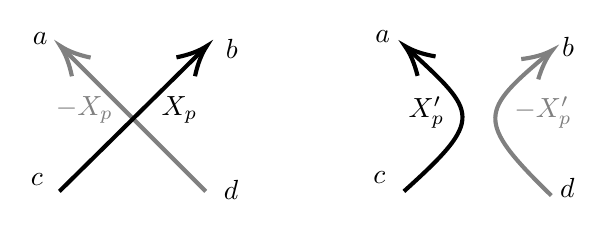
\begin{tikzpicture}[x=0.75pt,y=0.75pt,yscale=-1,xscale=1]
%uncomment if require: \path (0,109); %set diagram left start at 0, and has height of 109

%Straight Lines [id:da7979059503936952] 
\draw [color={rgb, 255:red, 128; green, 128; blue, 128 }  ,draw opacity=1 ][line width=1.5]    (39.62,19.12) -- (107.5,87) ;
\draw [shift={(37.5,17)}, rotate = 45] [color={rgb, 255:red, 128; green, 128; blue, 128 }  ,draw opacity=1 ][line width=1.5]    (14.21,-6.37) .. controls (9.04,-2.99) and (4.3,-0.87) .. (0,0) .. controls (4.3,0.87) and (9.04,2.99) .. (14.21,6.37)   ;
%Straight Lines [id:da7279842833116223] 
\draw [color={rgb, 255:red, 0; green, 0; blue, 0 }  ,draw opacity=1 ][line width=1.5]    (105.86,19.11) -- (37,87) ;
\draw [shift={(108,17)}, rotate = 135.41] [color={rgb, 255:red, 0; green, 0; blue, 0 }  ,draw opacity=1 ][line width=1.5]    (14.21,-6.37) .. controls (9.04,-2.99) and (4.3,-0.87) .. (0,0) .. controls (4.3,0.87) and (9.04,2.99) .. (14.21,6.37)   ;
%Curve Lines [id:da5605408166706283] 
\draw [color={rgb, 255:red, 0; green, 0; blue, 0 }  ,draw opacity=1 ][line width=1.5]    (203,87) .. controls (242.2,51.72) and (238.18,49.09) .. (205.53,18.88) ;
\draw [shift={(203.5,17)}, rotate = 402.85] [color={rgb, 255:red, 0; green, 0; blue, 0 }  ,draw opacity=1 ][line width=1.5]    (14.21,-6.37) .. controls (9.04,-2.99) and (4.3,-0.87) .. (0,0) .. controls (4.3,0.87) and (9.04,2.99) .. (14.21,6.37)   ;
%Curve Lines [id:da8925010918239024] 
\draw [color={rgb, 255:red, 128; green, 128; blue, 128 }  ,draw opacity=1 ][line width=1.5]    (274,89) .. controls (236.76,52.74) and (239.86,48.17) .. (272.47,20.71) ;
\draw [shift={(274.5,19)}, rotate = 499.95] [color={rgb, 255:red, 128; green, 128; blue, 128 }  ,draw opacity=1 ][line width=1.5]    (14.21,-6.37) .. controls (9.04,-2.99) and (4.3,-0.87) .. (0,0) .. controls (4.3,0.87) and (9.04,2.99) .. (14.21,6.37)   ;

% Text Node
\draw (23,9.4) node [anchor=north west][inner sep=0.75pt]    {$a$};
% Text Node
\draw (116,12.4) node [anchor=north west][inner sep=0.75pt]    {$b$};
% Text Node
\draw (22,77.4) node [anchor=north west][inner sep=0.75pt]    {$c$};
% Text Node
\draw (115,80.4) node [anchor=north west][inner sep=0.75pt]    {$d$};
% Text Node
\draw (85,40) node [anchor=north west][inner sep=0.75pt]  [color={rgb, 255:red, 0; green, 0; blue, 0 }  ,opacity=1 ]  {$X_p$};
% Text Node
\draw (34,40) node [anchor=north west][inner sep=0.75pt]  [color={rgb, 255:red, 128; green, 128; blue, 128 }  ,opacity=1 ]  {$-X_p$};
% Text Node
\draw (188,8.4) node [anchor=north west][inner sep=0.75pt]    {$a$};
% Text Node
\draw (278,11.4) node [anchor=north west][inner sep=0.75pt]    {$b$};
% Text Node
\draw (187,76.4) node [anchor=north west][inner sep=0.75pt]    {$c$};
% Text Node
\draw (277,79.4) node [anchor=north west][inner sep=0.75pt]    {$d$};
% Text Node
\draw (204,40) node [anchor=north west][inner sep=0.75pt]  [color={rgb, 255:red, 0; green, 0; blue, 0 }  ,opacity=1 ]  {$X'_p$};
% Text Node
\draw (255,40) node [anchor=north west][inner sep=0.75pt]  [color={rgb, 255:red, 128; green, 128; blue, 128 }  ,opacity=1 ]  {$-X'_p$};


\end{tikzpicture}
    \caption{$X_{p}$ and $X'_{p}$}
    \label{fig:crossing}
\end{figure}

Next we show that a generating set of $R(D)$ can be given by considering a spanning tree of the Seifert graph of $D$.
For each crossing $p$ of $D$, we define $X_{p}, X'_{p} \in R(D)$ by
\begin{align*}
    X_p &= x_b - x_c = -(x_a - x_d), \\
    X'_p &= x_a - x_c = -(x_b - x_d),
\end{align*}
where $a, b$ are outgoing edges at $p$ and $c,d$ are incoming edges at $p$, and $a, c$ are placed to the left of $p$ (see \Cref{complex,fig:crossing}).

\begin{lemma}[\cite{Nak20}]\label{treebasislem}
    Let $T$ be a spanning tree of the Seifert graph of $D$, and $S$ the set of crossings in $D$ corresponding to the edges of $T$.
    Then, $\mathcal{X}_T = \{X_p\}_{p \in S} \cup \{X'_p\}_{p \notin S}$ is an algebraically independent generating set of $R(D)$.
\end{lemma}

\begin{figure}
    \centering
    \tikzset{every picture/.style={line width=0.75pt}} %set default line width to 0.75pt        

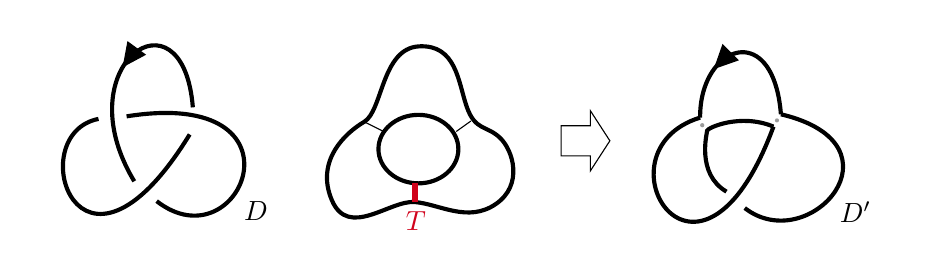
\begin{tikzpicture}[x=0.75pt,y=0.75pt,yscale=-1,xscale=1]
%uncomment if require: \path (0,109); %set diagram left start at 0, and has height of 109

\clip (0,0) rectangle (420,100);

%Curve Lines [id:da8161601596307948] 
\draw [line width=1.5]    (79.58,38.39) .. controls (74.8,-21.4) and (17.36,17.84) .. (51.36,74.01) ;
\draw [shift={(45.72,19.12)}, rotate = 306.15999999999997] [fill={rgb, 255:red, 0; green, 0; blue, 0 }  ][line width=0.08]  [draw opacity=0] (11.61,-5.58) -- (0,0) -- (11.61,5.58) -- cycle    ;
%Curve Lines [id:da5647400415250446] 
\draw [line width=1.5]    (62.15,83.58) .. controls (102.85,115.24) and (138.02,28.21) .. (47.66,42.73) ;
%Curve Lines [id:da13846906868786935] 
\draw [line width=1.5]    (34.13,43.95) .. controls (-3.3,51.35) and (24.68,138.29) .. (78.06,51.44) ;
%Curve Lines [id:da237486702787586] 
\draw [line width=1.5]    (362.91,41.73) .. controls (362.73,39.45) and (362.47,37.31) .. (362.15,35.31) .. controls (356.65,1.83) and (331.88,7.57) .. (325.49,31.04) .. controls (324.49,34.73) and (323.94,38.84) .. (323.99,43.32) ;
%Curve Lines [id:da6079162773576449] 
\draw [line width=1.5]    (345.48,86.91) .. controls (376.67,111) and (424.67,56.33) .. (362.91,41.73) ;
%Curve Lines [id:da012895447238909785] 
\draw [line width=1.5]    (323.99,43.32) .. controls (271.33,59.67) and (323.33,145) .. (359.33,47.67) ;
%Curve Lines [id:da4889524635526027] 
\draw [line width=1.5]    (359.33,47.67) .. controls (343.33,41) and (327.33,48.33) .. (327.33,49.67) .. controls (327.33,51) and (322,70.33) .. (336.67,79) ;
%Flowchart: Connector [id:dp9085114377251573] 
\draw  [draw opacity=0][fill={rgb, 255:red, 155; green, 155; blue, 155 }  ,fill opacity=1 ] (323.97,46.98) .. controls (323.97,46.42) and (324.43,45.96) .. (324.99,45.96) .. controls (325.55,45.96) and (326.01,46.42) .. (326.01,46.98) .. controls (326.01,47.54) and (325.55,48) .. (324.99,48) .. controls (324.43,48) and (323.97,47.54) .. (323.97,46.98) -- cycle ;
%Flowchart: Connector [id:dp9045304281632592] 
\draw  [draw opacity=0][fill={rgb, 255:red, 155; green, 155; blue, 155 }  ,fill opacity=1 ] (360,44.67) .. controls (360,44.11) and (360.45,43.67) .. (361,43.67) .. controls (361.55,43.67) and (362,44.11) .. (362,44.67) .. controls (362,45.22) and (361.55,45.67) .. (361,45.67) .. controls (360.45,45.67) and (360,45.22) .. (360,44.67) -- cycle ;
%Shape: Polygon Curved [id:ds49799004625007537] 
\draw  [line width=1.5]  (162.13,45.37) .. controls (171.07,40.12) and (170.5,10) .. (188.5,9) .. controls (206.5,8) and (207.42,26.18) .. (211.5,38) .. controls (215.58,49.82) and (221.05,46.9) .. (227.5,53) .. controls (233.95,59.1) and (238.94,75.83) .. (225.5,85) .. controls (212.06,94.17) and (198.5,85) .. (186.5,84) .. controls (174.5,83) and (154.5,102) .. (146.5,83) .. controls (138.5,64) and (153.18,50.62) .. (162.13,45.37) -- cycle ;
%Shape: Ellipse [id:dp8656777374199306] 
\draw  [line width=1.5]  (169,58.5) .. controls (169,49.39) and (177.62,42) .. (188.25,42) .. controls (198.88,42) and (207.5,49.39) .. (207.5,58.5) .. controls (207.5,67.61) and (198.88,75) .. (188.25,75) .. controls (177.62,75) and (169,67.61) .. (169,58.5) -- cycle ;
%Straight Lines [id:da1480688684375554] 
\draw    (162.13,45.37) -- (171.5,50) ;
%Straight Lines [id:da3873077880987402] 
\draw    (213.5,45) -- (206.5,50) ;
%Straight Lines [id:da043234858474899274] 
\draw [color={rgb, 255:red, 208; green, 2; blue, 27 }  ,draw opacity=1 ][line width=2.25]    (186.5,75) -- (186.5,84) ;
%Straight Lines [id:da23585575290034488] 
\draw [line width=1.5]    (335.5,15) -- (333.33,17.17) ;
\draw [shift={(330.5,20)}, rotate = 315] [fill={rgb, 255:red, 0; green, 0; blue, 0 }  ][line width=0.08]  [draw opacity=0] (11.61,-5.58) -- (0,0) -- (11.61,5.58) -- cycle    ;
%Right Arrow [id:dp28729390632428686] 
\draw   (257,47.25) -- (271.1,47.25) -- (271.1,40) -- (280.5,54.5) -- (271.1,69) -- (271.1,61.75) -- (257,61.75) -- cycle ;

% Text Node
\draw (103,82.4) node [anchor=north west][inner sep=0.75pt]    {$D$};
% Text Node
\draw (390,82.4) node [anchor=north west][inner sep=0.75pt]    {$D'$};
% Text Node
\draw (181,87.4) node [anchor=north west][inner sep=0.75pt]    {$\textcolor[rgb]{0.82,0.01,0.11}{T}$};


\end{tikzpicture}
    \caption{$D, T$ and $D'$}
    \label{fig:treebasislem}
\end{figure}

\begin{proof}
    Working over $\QQ$ allows us to have the equation
    \[
    \QQ[x_1, \ldots , x_m] = \QQ[x_1-x_2,\ x_2-x_3,\ \ldots,\ x_{m-1}-x_m,\ x_1+\cdots+x_m].
    \]
    Thus it follows that $R(D)$ is generated by elements of the form $x_e - x_f$, where $e, f$ are edges of $G(D)$.
    Since $|\mathcal{X}_T| = n$, it is enough to show that each $x_e - x_f$ can be written as a linear sum of elements in $\mathcal{X}_T$.
    Since $D$ is connected, by resolving all crossings in $D$ which are not in $S$, we obtain a diagram $D'$ of the trivial knot (see \Cref{fig:treebasislem} for an easy case).
    There is a unique oriented path $\gamma$ in $G(D')$ from $f$ to $e$, which may be also regarded as a path in $G(D)$.
    Trace $\gamma$ from $x_f$ to $x_e$, and each time $\gamma$ passes a crossing $p$ in $D$, take a term $\pm X_p$ or $\pm X'_p$ according to how $\gamma$ passes $p$ (see \Cref{fig:crossing}).
    It is obvious that these terms belong to $\mathcal{X}_T$ and that the sum gives $x_e-x_f$.
\end{proof}

\subsection{Reinterpretation as cube complexes} \label{subsec:double-cube-cpx}

Next we reinterpret the chain complex $C(D)$ given in \Cref{sec:prelim} as a ``double cube complex". Precise statement follows.

The \textit{$n$-cube} is a poset $\{0, 1\}^n$ with the product order of $0 < 1$, considered as a category.
An object $v \in \{0, 1\}^n$ is called a \textit{vertex}, and the Manhattan norm of $v$ is denoted by $|v| = v_1 + \cdots + v_n$. A morphism $v \to w$ such that $|v| + 1 = |w|$ is denoted $v \to_1 w$ and called an \textit{edge}. Define vertices $\bar{0} = (0, \ldots, 0)$ and $\bar{1} = (1, \ldots, 1)$.

\begin{figure}
    \centering
    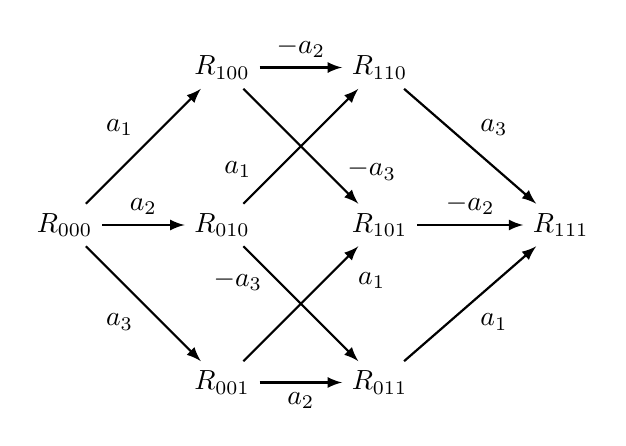
\begin{tikzpicture}[auto]
    \node (v0) at (-3.5,0.5) {$R_{000}$};
    \node (v1) at (-1.5,2.5) {$R_{100}$};
    \node (v2) at (-1.5,0.5) {$R_{010}$};
    \node (v3) at (-1.5,-1.5) {$R_{001}$};
    \node (v4) at (0.5,2.5) {$R_{110}$};
    \node (v5) at (0.5,0.5) {$R_{101}$};
    \node (v6) at (0.5,-1.5) {$R_{011}$};
    \node (v7) at (2.8,0.5) {$R_{111}$};
    \draw[-latex, thick] (v0) to node {$a_1$} (v1);
    \draw[-latex, thick] (v0) to node {$a_2$} (v2);
    \draw[-latex, thick] (v0) to node[swap] {$a_3$} (v3);
    \draw[-latex, thick] (v1) to node {$-a_2$} (v4);
    \draw[-latex, thick] (v1) edge (v5);
    \draw[-latex, thick] (v2) edge (v4);
    \draw[-latex, thick] (v2) edge (v6);
    \draw[-latex, thick] (v3) edge (v5);
    \draw[-latex, thick] (v3) to node[swap] {$a_2$} (v6);
    \draw[-latex, thick] (v4) to node {$a_3$} (v7);
    \draw[-latex, thick] (v5) to node {$-a_2$} (v7);
    \draw[-latex, thick] (v6) to node[swap] {$a_1$} (v7);
    \node at (0.4,-0.2) {$a_1$};
    \node at (0.4,1.2) {$-a_3$};
    \node at (-1.3,-0.2) {$-a_3$};
    \node at (-1.3,1.2) {$a_1$};
\end{tikzpicture}

    \caption{A cube complex with factors $(a_1, \ldots, a_n)$.}
    \label{fig:cube-complex}
\end{figure}

Let $\mathcal{A}$ be an additive category.
\begin{definition}
    For $n \geq 0$, an \textit{$n$-cube in $\mathcal{A}$} is a functor $\mathcal{C}\colon \{0, 1\}^n \to \mathcal{A}$.
\end{definition}

Given an $n$-cube $\mathcal{C}$ in $\mathcal{A}$,
one obtains a \textit{cube complex} $(C^*, d^*)$ in $\mathcal{A}$ with 
\[
    C^i = \bigoplus_{|v| = i} \mathcal{C}(v)
\]
and differentials
\[
    d^i = \sum_{\substack{|v| = i,\\ e\colon v \to w}} s(e)\mathcal{C}(e),
\]
by choosing $s(e) \in \{\pm 1\}$ for each edge $e$ of the cube so that for any square consisting of four edges $e_1,\ldots,e_4$, we have $s(e_1) \cdots s(e_4) = -1$.

\begin{remark}
    The isomorphism class of the above cube complex is independent of the choice of $s$.
\end{remark}

Now we put $C(D)$ in this framework. First we will ignore the original homological gradings, and lately relate them with the newly introduced gradings. 
%
We recall that $C(D)$ is a tensor product of (vertical) two-terms complexes of (horizontal) complexes. Hence $C(D)$ can be regarded as a cube complex of complexes. We write 
\[
    C(D) = \bigoplus_{v \in \{0, 1\}^n} C^*_v(D),
\]
where $C^*_v(D)$ is the complex at a vertex $v \in \{0, 1\}^n$, called the \textit{horizontal complex} of $D$ at $v$.
Since $C^*_v(D)$ is also a tensor product of two-terms complex over $R(D)$, it can be regarded as a cube complex again. We write
\[
    C^*_v(D) = \bigoplus_{h \in \{0, 1\}^n} R_{v, h}(D),
\]
where $R_{v, h}(D)$ is the module at a vertex $h \in \{0, 1\}^n$, and it is indeed a shifted copy of $R(D)$. The horizontal differential 
\[
    d_H: C^*_v(D) \rightarrow C^{*+1}_v(D)
\]
has the following form.
For each standard unit vector $e_i$ of $\RR^n$, there exists an element $a_i$ of $R(D)$ such that for any edge $v \to_1 w$ in the direction of $e_i$ in the $n$-cube, the corresponding map $R_{v,h}(D) \to R_{w,h}(D)$ summed in $d_H$ is the multiplication map by $a_i$ as specified by the horizontal arrows of \Cref{complex} according to $v$ (with some appropriate sign assignment). We call $a_1, \ldots, a_n$ the \textit{factors} of $C^*_v(D)$ (see \Cref{fig:cube-complex}).

By taking the homology with respect to $d_H$, we get a cube complex of homologies
\[
    \bigoplus_{v \in \{0, 1\}^n} H^*(C_v(D), d_H)
\]
with differential $(d_V)_*$. Then it is obvious that $\Hhat(D)$ is given by the homology of this complex
\[
    \Hhat(D) = H(\oplus_v (H(C_v(D), d_H), (d_V)_*).
\]

The homological bigrading $(\alpha, \beta)$ of the double cube complex $C(D)$ correspond to the original bigrading $(j, k)$ as
\[
    (\alpha, \beta) = \frac{1}{2}(j - j_0,\ k - k_0)
\]
where $(j_0, k_0)$ is the (original) homological bidegree of the module $R_{\bar{0}, \bar{0}}(D)$ placed at $(v, h) = (\bar{0}, \bar{0})$. For later use, let $i_0$ denote the $q$-grading shift of $R_{\bar{0}, \bar{0}}(D)$. Then from \Cref{complex} we have 
%
\begin{equation} \label{eq:ijk0}
    (i_0, j_0, k_0) = (2n^+, -2n, -2n^+)
\end{equation}
%
where $n_+$ and $n_-$ are the number of positive and negative crossings of $D$ respectively.

\subsection{Slicing by $q$-degrees} 

As described in \Cref{treebasislem}, the ring $R(D)$ can be represented by a multivariate polynomial ring $\QQ[X_i]$ with $n$ variables, so we have a homogeneous decomposition of $R(D)$ as a $\QQ$-vector space
\[
    R(D) \isom \QQ(1) \oplus \QQ(X_i)_{1 \leq i \leq n}  \oplus \QQ(X_i X_j)_{1 \leq i \leq j \leq n} \cdots.
\]
Let $i_{v, h} \in \ZZ$ be the $q$-grading shift of $R_{v, h}(D) = R(D)\{i_{v, h}\}$. Decompose $R_{v, h}(D)$ as 
\[
    R_{v, h}(D) = \bigoplus_{l = -\infty}^\infty V_{l, v, h}(D)
\]
so that each $V_{l, v, h}(D)$ is homogeneous of $q$-degree $2(l + |h|) + i_0$. It is generated by monomials 
% $X_{i_1} \cdots X_{i_e}$ 
of degree (in the usual sense) 
%
\begin{equation} \label{eq:monomial-degree}
    e(l, v, h) = l + |h| + \frac{i_0 - i_{v, h}}{2}.
\end{equation}
%
Now define 
\[
    C_l(D) = \bigoplus_{v, h} V_{l, v, h}(D)
\]
then it is obvious that both $d_H, d_V$ are closed in $C_l(D)$.  Regarding $C(D)$ as a chain complex over $\QQ$, we get a decomposition
\[
    C(D) = \bigoplus_{l = -\infty}^\infty C_l(D).
\]
We call each subcomplex $C_l(D)$ the \textit{level-$l$ slice} of $C(D)$. Note that the decomposition is defined so that $V_{l, \bar{0}, \bar{0}}(D)$ is generated by monomials of degree $e = l$. 

\begin{lemma}
    $C_l(D) = 0$ for $l < -2n$.
\end{lemma}

\begin{proof}
    The claim is clear since $e$ is non-decreasing with respect to $v, h$ and $e(l, \bar{1}, \bar{1}) = l + 2n$.
\end{proof}

From the previous arguments, it is obvious that each $C_l(D)$ may also be regarded as a double cube complex. Define the \textit{level-$l$ slice} $C_{l, v}(D)$ of the horizontal complex $C_v(D)$ at $v \in \{0, 1\}^n$ by
\[
    C_{l, v}(D) = \bigoplus_{h \in \{0, 1\}^n} V_{l, v, h}(D).
\]
Then we get a decomposition
\[
    \Hhat(D) = \bigoplus_{l = -2n}^\infty \Hhat_l(D),
\]
where 
\[
    \Hhat_l(D) = H(\oplus_v (H(C^*_{l, v}(D), d_H), (d_V)_*).
\]

We claim that each $\Hhat_l(D)$ is algorithmically computable. To take the homology twice, we find a basis on each chain group $C^i = C^i_{l, v}(D)$ that gives a decomposition
\[
    C^i = H^i \oplus B^i \oplus (d^i_H)^{-1}(B^{i + 1})
\]
so that we get representative cycles of the generators of $H^i = H^i(C^*_{l, v}(D))$ and that the secondary homology computation can be done on the chain level. This is achieved by standard methods such as the Gaussian elimination. 

\begin{proposition}
    For a link diagram $D$, the homology $\Hhat(D)$ has a decomposition
    \[
        \Hhat(D) = \bigoplus_{l = -2n}^{\infty} \Hhat_l(D)
    \]
    where each summand $\Hhat_l(D)$ can be computed algorithmically. Moreover for each triple degree $(i, j, k)$ we have 
    %
    \begin{equation} \label{eq:Hijk}
        \Hhat^{i, j, k}(D) = H^\beta(\oplus_v (H^\alpha(C^*_{v, l}(D), d_H), (d_V)_*)
    \end{equation}
    %
    where
    %
    \[
        (l, \alpha, \beta) = \frac{1}{2}((i - i_0) - (j - j_0),\ j - j_0,\ k - k_0)
    \]
    and $(i_0, j_0, k_0)$ are given as in \eqref{eq:ijk0}. Similar statement holds for $\Hbar(D)$. \qed
\end{proposition}

Now we restrict to the case where $D$ is a knot diagram, and in particular where it is a braid closure. In such case, it is well-known that $\Hbar(D)$ is finite dimensional \cite{Ras15}. In order to perform the actual calculation, we must specify an actual upper bound for the level $l$.

\begin{proposition} \label{prop:finiteness}
    If $K$ is a knot with braid closure diagram $D$, then
    \[
        \Hbar(K) \isom \bigoplus_{l = -2n}^{-n} \Hbar_l(D).
    \]
    Moreover, $\Hbar(K)$ can be obtained from the computations of $\Hbar^{i, j, k}(D)$ within the following ranges:
    \begin{align*}
        i &\in [-n + s - 1, 0], \tag{1}\\
        j &\in [w - s + 1, w + s - 1], \tag{2}\\
        k,\ k + 2i &\in [-n + s - 1, n - s + 1]. \tag{3}
    \end{align*}
\end{proposition}

\begin{proof}
    From \Cref{prop:MFW-ineq,prop:morton} and equation \eqref{eq:Hbar-def}, it follows that $\Hbar_l(D)$ is supported in 
    \begin{align*}
        2l 
        &= (i - i_0) - (j - j_0) \\ 
        &\leq \{ (n - s + 1) - (-w + s - 1) - 2n^+ \}\\
        &\quad - \{(w - s + 1) - (w + s - 1) - (-2n)\}\\
        &= -2n.
    \end{align*}
    For the latter statement: (1) the lower bound is given by the Morton bound (\Cref{prop:morton}), and from \Cref{prop:q-sym} it suffices to compute $H^{i, *, *}(D)$ within $i \leq 0$.
    (2) This is exactly \Cref{prop:MFW-ineq}.
    (3) The lower bound of $k$ is obvious from the definition of $C(D)$, and from \Cref{prop:duality} we also have the upper bound. From \Cref{prop:q-sym}, $k + 2i$ must also lie in this range.
\end{proof}

\subsection{Exclusion of variables}

As apparent from \eqref{eq:monomial-degree}, the number of generators increases combinatorially as $l$ increases. In order to reduce the computational cost, we use the process called ``exclusion of variables" as described in \cite[Lemma 3.8]{Ras15}. 

Again we assume $D$ is a link diagram. Put $R = R(D)$. Take any $v \in \{0, 1\}^n$ and consider the horizontal cube complex $C = C_v(D)$. Take any factor $f \in R$ of $C$. Note that $f$ is either linear or quadratic.

After choosing an appropriate sign assignment, $C$ may be regarded as the mapping cone of the endomorphism 
\[
    C' \xrightarrow{f} C'
\]
of an $n-1$ dimensional cube complex $C'$. Let $d, d'$ denote the differentials of $C, C'$ respectively. The complex $C$ is isomorphic to $C' \oplus C'$ as an $R$-module, and we can write
\[
    d(x_0, x_1) = (-d'x_0, fx_0 + d'x_1).
\]

Now $f$ is monic with respect to some variable $X_k$. Define
\[
R_0 = \QQ[X_1, \ldots \widehat{X_k}, \ldots, X_n].
\]
Let $\pi \colon R \rightarrow R_1 = R/(f)$ be the quotient map, $\iota \colon R_1 \rightarrow R$ be the map that sends any residue class $[g] \in R_1$ to the remainder of $g$ by $f$ with respect to the variable $X_k$.
We note that $\pi$ and $\iota$ are homomorphisms of modules over $R$ and $R_0$ respectively.
Let $C'' = C' \otimes_R R_1$, and let $d''$ be the differential of $C''$. Two chain maps $\phi \colon C \rightarrow C''$ and $\psi \colon C'' \rightarrow C$ over $R_0$ are given by
\[
    \phi(x_0, x_1) = \pi(x_1),
\]
and
\[
    \psi(y) = \left(\frac{\iota(d''y) - d'\iota(y)}{f},\  \iota(y)\right),
\]
and it is not hard to verify that $\psi \phi \htpy \id_C$ and $\phi \psi = \id_{C''}$.
The complex $C''$ admits the obvious triple grading so that both $\phi, \psi$ are degree preserving. Thus the two maps restrict as chain homotopy equivalences between the two sliced complexes $C_l$ and $C''_l$. The effect is that $H(C_l) \cong H(C''_l)$ can be computed with fewer generators, which is drastic when $l$ becomes large. 

Furthermore, this process of reduction can be repeated for other directions as long as the target variable is algebraically independent in the base ring. When $f$ is linear, we have $R_1 \isom R_0$ and all other variables remain independent. When $f$ is quadratic, then $R_1 \isom R_0 \otimes_\QQ \QQ\{1, X_k\}$ as $\QQ$-vector spaces, and the variables that does not appear in the coefficients of $f$ remains independent.

In particular, when all factors $f$ of $C$ are linear, then the exclusion can be continued until the differential becomes trivial. In general, to exclude the variables as much as possible, it is preferable to perform exclusions on linear polynomials first, and then on the remaining quadratics. 

For the computation of $\Hbar(D)$, we can replace each horizontal complex $C_{l, v}$ with a reduced one, compute those homologies, and replace the differential $(d_V)_*$ on the vertical complex with $(\phi_{v'} \circ d_V \circ \psi_v)_*$ for each edge $v \rightarrow v'$. 

\subsection{Overall procedure}

We summarize the overall procedure for computing (the dimensions of) the reduced HOMFLY homology $h^{i, j, k} = \{\dim \Hbar^{i, j, k}(K)\}_{i, j, k}$ of a knot $K$.

\begin{algorithm}\label{algo:basic}
    Given a braid closure diagram $D$ of a knot $K$, 
    \begin{enumerate}
        \item Compute the Seifert graph $G(D)$ and find a spanning tree $T$ of $G(D)$. 
        
        \item Using $T$, identify the edge ring $R(D)$ as a multivariate polynomial ring, and represent both $d_H$ and $d_V$ as $n$-tuples of polynomials in $R(D)$ as in the proof of \Cref{treebasislem}.
        
        \item For each $(l, \alpha, \beta)$ in $[-2n, -n] \times [0, n] \times [0, n]$:
        \begin{enumerate}
            \item Convert $(l, \alpha, \beta)$ to $(i, j, k)$. Skip to the next iteration if $(i, j, k)$ is not in the range of \Cref{prop:finiteness}.
            
            \item Setup the generators of the level-$l$ horizontal complex $C_l(D)$.
            
            \item Perform exclusion of variables on $C_l(D)$ to get a reduced complex together with the chain homotopy equivalences. 

            \item Compute $h^{i, j, k} = \dim \Hbar^{i, j, k}(D)$ from \eqref{eq:Hijk}, with the horizontal complexes replaced with the reduced ones. 
            
            \item Assign $h^{-i, j, k + 2i} = h^{i, j, k}$ if $i < 0$.
        \end{enumerate}
        \item Return $h$.
    \end{enumerate}
\end{algorithm}

Reusable data should be cached within the iteration. Further improvement can achieved by concerning mirrors of knots. To explain this, assume that $D$ has only one crossing $p$. Recall that the vertex module $V_{l, v, h}(D)$ at $(v, h) \in \{0, 1\}^2$ is spanned by the monomials of degree given  by \eqref{eq:monomial-degree}. From \Cref{complex}, we see that $e(l, 1, 0) = e(l, 0, 1) = e(l, 0, 0) + 1$ if $p$ is positive, and $e(l, 1, 0) = e(l, 0, 1) = e(l, 0, 0)$ if $p$ is negative (in both cases $e(l, 1, 1) = e(l, 0, 0) + 1$). This means that $C_l(D)$ has a smaller generating set when $p$ is negative. In general if $w(D) > 0$, then $C_l(m(D))$ has a smaller generating set than $C_l(D)$. This difference becomes intense as $n$ increases. Thus the improved version is:

\begin{algorithm}\label{algo:mirror}
    Given a braid closure representative $D$ of a knot $K$, \begin{enumerate}
        \item If $w(D) \leq 0$, compute and return $h(D)$ by \Cref{algo:basic}.
        \item Otherwise, compute $h(m(D))$ by \Cref{algo:basic} and return its dual.
    \end{enumerate}
\end{algorithm}
\section{Skyline Computation Over Categorical Attributes}\label{sec:3}
Without loss of generality, for ease of explanation, we consider a relation with Boolean attributes, i.e., categorical attributes with domain size 2. We shall discuss the extensions of the algorithms for categorical attributes with larger domains later in this section.

Throughout this section, we consider the case in which precomputed indices are not available. First, we exploit the categorical characteristics of attributes by designing a tree data structure that can perform efficient {\em dominance} operations. Specifically, given a new tuple $t$, the tree supports three primitive operations -- i) INSERT($t$): inserts a new tuple $t$ to the tree, ii) IS-DOMINATED($t$): checks if tuple $t$ is dominated by any tuple in the tree, and iii) PRUNE-DOMINATED-TUPLES($t$): deletes the tuples dominated by $t$ from the tree. In Appendix \ref{ap:tree-optimizations}, we further improve the performance of these basic operations by proposing several optimization techniques. Finally, we propose two algorithms ST-S (Skyline using Tree Sorting-based) and ST-P (Skyline using Tree Partition-based) that incorporate the tree structure to state-of-art sorting- and partition-based algorithms.


\subsection{Organizing Tuples Tree}\label{subsec:tree}
\vspace{1mm}
\noindent{\bf Tree structure:} We use a binary tree to store tuples in the candidate skyline set. Consider an ordering of all attributes in $\mathcal{Q} \subseteq \mathcal{A}$, e.g., $[A_1, A_2, \ldots, A_{m'}]$.
In addition to tuple attributes, we enhance each tuple with a score, assessed using a function $F(\cdot)$. This score assists in improving performance during identification of the dominated tuples or while conducting the dominance check. The proposed algorithm is agnostic to the choice of $F(\cdot)$; the only requirement is that the function does not assign a higher score to a dominated tuple compared to its dominator.
The structure of the tree for Example~\ref{exmp:ST} is depicted in Figure~\ref{fig:tree}. The tree has a total of 5 ($=m'+ 1$) levels, where the $i$'th level ($1 \leq i \leq m'$) represents attribute $A_i$. The left (resp. right) edge of each internal node represents value 0 (resp. 1). Each path from the root to a leaf represents a specific assignment of attribute values. The leaf nodes of the tree 
store two pieces of information: i) $score$: the score of the tuple mapped to that node, and ii) \textit{tupleID List}: list of ids of the tuples mapped to that node. Note that all the tuples that are mapped to the same leaf node in the tree have the same attribute value assignment, i.e. have the same score.
Moreover, the attribute values of a tuple $t$ can be identified by inspecting the path from the root to a leaf node containing $t$. Thus, there is no requirement to store the attribute values of the tuples in the leaf nodes.
Only the leaf nodes that correspond to an actual tuple are present in the tree. 

\begin{exmp}\label{exmp:ST} 
As a running example through out this section, consider the relation $D$ with $n=5$ non-dominated tuples where its projection on $\mathcal{Q}=\{A_1,A_2,A_3,A_4\}$ is depicted in Table~\ref{tab:skylineTreeRunningExample}. 
The last column of the table presents the score of each tuple, utilizing the function $F(\cdot)$  provided in Equation~\ref{eq:score}.
\begin{align}\label{eq:score}
F(t_{\mathcal{Q}}) = \sum_{A_i \in \mathcal{Q}} 2^{i-1} \cdot t[A_i]
\end{align}
\end{exmp}



\begin{table}[!t]
\centering
\caption{Example~\ref{exmp:ST} relation}\label{tab:skylineTreeRunningExample}
\begin{tiny}
\begin{tabular}{cccccc}
    \hline 
    $tupleID$ & $A_1$ & $A_2$ & $A_3$ & $A_4$ & $Score$\\
    \hline 
    $t_1$ & 1 & 1 & 0 & 0 & 12\\
    \hline
    $t_2$ & 0 & 0 & 1 & 1 & 3\\
    \hline
    $t_3$ & 0 & 1 & 1 & 0 & 6\\
    \hline
    $t_4$ & 1 & 0 & 0 & 1 & 9\\
    \hline
    $t_5$ & 1 & 0 & 1 & 0 & 10\\
    \hline
\end{tabular}
\end{tiny}
\end{table}

\begin{figure*}[!t]
\begin{minipage}[t]{0.23\linewidth}
\centering
    \includegraphics[scale=0.80]{figures/SkylineTree.pdf}
    %\vspace{-8mm}
    \caption{Tree structure for relation in Example~\ref{exmp:ST}}
    \label{fig:tree}
\end{minipage}
\hspace{1mm}
\begin{minipage}[t]{0.23\linewidth}
\centering
    \includegraphics[scale=0.80]{figures/SkylineTreeDominate.pdf}
    %\vspace{-8mm}
    \caption{Prune dominated tuples}
    \label{fig:treePruneDominatedTuples}
\end{minipage}
\hspace{1mm}
\begin{minipage}[t]{0.23\linewidth}
\centering
    \includegraphics[scale=0.80]{figures/SkylineTreeDominateAfter.pdf}
    %\vspace{-8mm}
    \caption{Tree after removing dominated tuples}
    \label{fig:treePruneDominatedTuplesAfter}
\end{minipage}
\hspace{1mm}
\begin{minipage}[t]{0.23\linewidth}
\centering
    \includegraphics[scale=0.80]{figures/SkylineTreeDominated.pdf}
    %\vspace{-8mm}
    \caption{Check if tuple $t$ is dominated}
    \label{fig:treeCheckIfDominated}
\end{minipage}
\end{figure*}


\vspace{1mm}
\noindent{\bf INSERT($t$):} In order to insert a tuple $t$ into the tree, we start from the root. At level $i$ $(1 \leq i \leq m')$, we check the corresponding attribute value, $t[A_i]$. If $t[A_i] = 0$ (resp. $t[A_i] = 1$) and the left (resp. right) child of current node already exists in the tree, we simply follow the left (resp. right) child. Otherwise, we first have to create a new tree node as left (resp. right) child before traversing it. After reaching the leaf node at level $m'+1$, the $tupleID$ of $t$ is appended to \textit{tupleID List} and the $score$ value is assigned to newly constructed leaf.

\begin{algorithm}[!htb]
\caption{{\bf INSERT}}
\begin{algorithmic}[1]
\label{alg:insertTuple}
\STATE {\bf Input:} Tuple $t$, Node $n$, Level $l$, Query $\mathcal{Q}$;
%\STATE {\bf if} $n$ is $leaf$ node:
\STATE {\bf if} $l == |\mathcal{Q}| + 1$:
    \STATE \hindent {\bf if} $n.score$ is None: $n.score = score(t)$
    \STATE \hindent Append $t[tupleID]$ to $n.tupleIDList$
\STATE {\bf else}:
    \STATE \hindent {\bf if} $t[A_l]==0$:
        \STATE \hindent[2] {\bf if} $n.left$ is $None$:
           % \STATE \hindent[3] Create $left$ child of $t$
           \STATE \hindent[3] temp = {\it New} Node();
           \STATE \hindent[3] $t.left$ = temp;
        \STATE \hindent[2] INSERT($t$, $n.left$, $l+1$)
    \STATE \hindent {\bf if} $t[A_l]==1$:
        \STATE \hindent[2] {\bf if} $n.right$ is $None$:
           % \STATE \hindent[3] Create $right$ child of $t$
           \STATE \hindent[3] temp = {\it New} Node();
           \STATE \hindent[3] $t.right$ = temp;
        \STATE \hindent[2] INSERT($t$, $n.right$, $l+1$)
\end{algorithmic}
\end{algorithm}

\vspace{1mm}
\noindent{\bf PRUNE-DOMINATED-TUPLES($t$):} The pruning algorithm to delete from the tree, tuples dominated by $t$, is recursively developed as follows: We start from the root node of the tree. If $t[A_1] = 1$, we search both the left and right subtree. Otherwise, only the left child is selected. This is because if $t[A_1] = 1$, a tuple $t'$ dominated by $t$ can assume value  0 or 1 on attribute $A_1$. On the other hand, $t$ cannot dominate a tuple $t'$ if $t[A_1] = 0$ and $t'[A_1] = 1$. We follow the same approach at each internal node visited by the algorithm - at level $i$ $(1 \leq i \leq m)$, value of $t[A_i]$ is used to select the appropriate subtree. After reaching a leaf node, we compare $score(t_{\mathcal{Q}})$ with the $score$ value of leaf node. If both values are equal, no action is required, since, all the tuples mapped into the current leaf node have the same attribute value as $t_{\mathcal{Q}}$. Else, the leaf node is deleted from the tree. Upon return from the recursion, we check if both the left and right child of the current (internal) node are empty. In that case, the current node is also deleted from the tree.

Figure~\ref{fig:treePruneDominatedTuples} demonstrates the pruning algorithm for $t = \langle 1,0,1,1 \rangle$. Tuples in the tree that are dominated by $t$ are: $t_2$, $t_4$, and $t_5$. The bold edges represent paths followed by the pruning algorithm. Both the left and right children of node $a$ are visited since $t[A_1] = 1$, whereas, at nodes $f$ and $b$ only the left subtree is selected for searching. The final structure of the tree after deleting the dominated tuples is shown in Figure~\ref{fig:treePruneDominatedTuplesAfter}.

\begin{algorithm}[htb]
\caption{{\bf PRUNE-DOMINATED-TUPLES}}
\begin{algorithmic}[1]
\label{alg:pruneDominatedTuples}
\STATE {\bf Input:} Tuple $t$, Node $n$, Level $l$, Score $s$, Query $\mathcal{Q}$;

\STATE {\bf if} $n$ is $None$ or $n.minScore > s$ {\bf return}

\STATE {\bf if} $l == |\mathcal{Q}| + 1$ and $score(t_{\mathcal{Q}}) \neq n.score$:
    \STATE \hindent Delete $n$ from tree
    \STATE \hindent {\bf return}

\STATE {\bf if} $t[A_l] == 1$:
    \STATE \hindent PRUNE-DOMINATED-TUPLES($t$, $n.right$, $l+1$, $s$)
    \STATE \hindent $s' = s - weight(A_i)$
    \STATE \hindent PRUNE-DOMINATED-TUPLES($t$, $n.left$, $l+1$, $s'$)
\STATE {\bf else}:
    \STATE \hindent PRUNE-DOMINATED-TUPLES($t$, $n.left$, $l+1$, $s$)

\STATE {\bf if} Both $left$ and $right$ children of $n$ is $None$
    \STATE \hindent Delete $n$ from tree
\end{algorithmic}
\end{algorithm}


\vspace{1mm}
\noindent{\bf IS-DOMINATED($t$):} The algorithm starts traversing the tree from the root. For each node visited by the algorithm at level $i$ $(1 \leq i \leq m)$, we check the corresponding attribute value $t[A_i]$. If $t[A_i] = 0$, we search both the left and right subtree; otherwise, we only need to search in the right subtree. This is because when $t[A_i] = 0$, all the tuples dominating $t$ can be either 0 or 1 on attribute $A_i$. If we reach a leaf node that has an attribute value assignment which is different than that of $t$ (i.e., $score \neq score(t)$), $t$ is dominated.  Note that, when $t[A_i] = 0$ both the left and right subtree of the current node can have tuples dominating $t$, while the cost of identifying a dominating tuple (i.e., the number of nodes visited) may vary depending on whether the left or right subtree is visited first. For simplicity, we always search in the right subtree first. If there exists a tuple in the subtree of a node that dominates tuple $t$, we do not need to search in the left subtree anymore. 

Figure~\ref{fig:treeCheckIfDominated} presents the nodes visited by the algorithm in order to check if the new tuple $t = \langle 0,0,1,0 \rangle$ is dominated. We start from the root node $a$ and check the value of $t$ in attribute $A_1$. Since $t[A_1] = 0$, we first search in the right subtree of $a$. After reaching to node $d$, the algorithm back-tracks to $b$ (parent of $d$). This is because $t[A_3] = 1$ and $d$ has no actual tuple mapped under it's right child. Since $t[A_2] = 0$ and we could not identify any dominating tuple in the right subtree of $b$, the algorithm starts searching in the left subtree and moves to node $c$. At node $c$, only the right child is selected, since $t[A_3] = 1$. Applying the same approach at node $f$, we reach the leaf node $e$ that contains the tupleID $t_5$. Since the value of the $score$ variable at leaf node $e$ is different from $score(t)$, we conclude that tuples mapped into $e$ (i.e., $t_5$) dominate $t$.

Please refer to Appendix~\ref{ap:tree-optimizations} for further optimizations on the tree data structure.

\begin{algorithm}[htb]
\caption{{\bf IS-DOMINATED}}
\begin{algorithmic}[1]
\label{alg:isDominated}
\STATE {\bf Input:} Tuple $t$, Node $n$, Level $l$, Score $s$, Query $\mathcal{Q}$; \qquad {\bf Output:} True if $t$ is dominated else False.
\STATE {\bf if} $n$ is $None$ or $s > n.maxScore$: {\bf return}

\STATE {\bf if} $l == |\mathcal{Q}|$ and $score(t_{\mathcal{Q}}) \neq n.score$: {\bf return} True
\STATE {\bf if} $l == |\mathcal{Q}|$ and $score(t_{\mathcal{Q}}) = n.score$: {\bf return} False

\STATE {\bf if} $t[A_l] == 0$:
    \STATE \hindent $s' = s + weight(A_i)$
    \STATE \hindent $dominated$ = IS-DOMINATED($t$, $n.right$, $l+1$, $s'$)
    \STATE \hindent {\bf if} $dominated$ == True: {\bf return} True
    \STATE \hindent {\bf return} IS-DOMINATED($t$, $n.left$, $l+1$, $s$)
\STATE {\bf else}:
    \STATE \hindent {\bf return} IS-DOMINATED($t$, $n.right$, $l+1$, $s$)
\end{algorithmic}
\end{algorithm}



\subsection{Skyline using Tree}\label{sec:ST}

Existing works on skyline computation mainly focus on two optimization criteria: reducing the number of dominance checks (CPU cost), limiting communication cost with the backend database (I/O cost). Sorting-based algorithms reduce the number of dominance check by ensuring that only the skyline tuples are inserted in the candidate skyline list. Whereas, partition-based algorithms achieve this by skipping dominance tests among tuples inside incomparable regions generated from the partition. However, given a list of tuples $\mathcal{T}$ and a new tuple $t$, in order to discard tuples from $\mathcal{T}$ that are dominated by $t$, both the sorting- and partition-based algorithms need to compare $t$ against all the tuples in $\mathcal{T}$. This is also the case when we need to check whether $t$ is dominated by $T$. The tree structure defined in \S\ref{subsec:tree} allows us to perform these operations effectively for categorical attributes. Since the performance gain achieved by the tree structure is independent of the optimization approaches of previous algorithms, it is possible to combine the tree structure with existing skyline algorithms. We now present two algorithms ST-S (Skyline using Tree Sorting-based) and ST-P (Skyline using Tree Partition-based) that incorporates the tree structure into existing algorithm.

\vspace{1mm}
\noindent{\bf ST-S:} ST-S combines the tree structure with a sorting-based algorithm. Specifically, we have selected the SaLSa~\cite{bartolini2008efficient} algorithms that exhibits better performance compared to other sorting-based algorithms. The final algorithm is presented in Algorithm~\ref{alg:st-s}. The tuples are first sorted according to ``maximum coordinate'', maxC, criterion\footnote{Assuming larger values are preferred for each attribute.}. Specifically, Given a skyline query $\mathcal{Q}$, $maxC(t_{\mathcal{Q}}) = (max_{A\in \mathcal{Q}}\{t[A]\}, sum(t_{\mathcal{Q}}))$, where $sum(t_{\mathcal{Q}}) = \sum_{A\in \mathcal{Q}} t[A]$. A tree structure $T$ is used to store the skyline tuples. Note that the monotonic property of the scoring function $maxC(\cdot)$ ensures that all the tuples inserted in $T$ are skyline tuples. The algorithm then iterates over the sorted list one by one, and for each new tuple $t$, if $t$ is not dominated by any tuple in tree $T$, it is inserted in the tree (lines 7-8). For each new skyline tuple, the ``stop point'' $t_{stop}$ is updated if required (line 10-12). The algorithm stops if all the tuples are accessed or $t_{stop}$ dominates the remaining tuple. Detailed description of the ``stop point'' can be found in the original SaLSa paper~\cite{bartolini2008efficient}.


%%%%%%%%%%%%%%%%%%%%%%%%%%%%%%%%%%%%%%%%%%%%%%%%%%%%%%%%%%%%%%%%%%%%%%%%%%%%%%%%%%%%
%We now present the Skyline using Tree Algorithm (ST) that utilizes the tree data structure defined in \S\ref{subsec:tree} for discovering skylines.  Therefore, it is possible to incorporate the tree data structure into existing skyline algorithms and improve the performance further. The ST algorithm we are going to proposed in this section is adaption of stat-of-art sorting-based algorithm SaLSa~\cite{bartolini2008efficient}. The partition-based algorithms does not perform well for categorical attributes. Hence, are skipped from consideration (See \S\ref{sec:relWork} for details). We first start with a brief description of SaLSa and then describe how it can be incorporated with ST algorithm.

%Sorting based algorithms tries to reduce the total number of dominance test by discarding the no skyline points with fewer number of dominance test. This can be achieved by sorting the tuples in relation using a monotonic scoring function. In addition of sorting, . As the algorithm progress, SaLSa maintains a \textit{stopping point}, selected from the skylines that are already discovered. In addition it defines an {\em unread domain} that is dynamically updated after reading each point. The unread domain can be considered as an hyper rectangle that contains points that are yet to be accessed for dominance check. SaLSa stops when the stop point dominates the unread region. The authors also showed that the correctness and as well as performance of the algorithm depends on the choice of scoring function $F(\cdot)$. The number of tuples needed to be accessed can be minimized by sorting data according to ``maximum coordinate'', maxC, criterion\footnote{Assuming larger values are preferred for each attribute.}. Specifically, $maxC(t) = (min_j\{t[j]\}, sum(t))$, where $sum(t) = \sum_{j=1}^mp[j]$. 


%The final ST algorithm is presented in Algorithm~\ref{alg:st}. First, we sort the tuples in descending order of their maxC value. The algorithm then starts scanning tuples from the \textit{sorted list} one by one. For each new tuple $t$ ST checks whether the tuple is dominated by tuple $t'_\mathcal{Q}$ in $T$. If not $t$ is a skyline tuple and inserted in $T$. The stopping point $t_{stop}$ is updated if the minimum attribute value of current skyline tuple $t$ is grater then minimum attribute value of $t_{stop}$ (Line 10-11). The algorithm stops when all the tuples are accessed or $t_{stop}$ dominates the remaining tuples (Line 6). Note that sorting the tuples using a monotonic property of maxC function ensures that all the tuples inserted into $T$ are skyline in $D$.
%%%%%%%%%%%%%%%%%%%%%%%%%%%%%%%%%%%%%%%%%%%%%%%%%%%%%%%%%%%%%%%%%%%%%%%%%%%%%%%%%%%%

\begin{algorithm}[htb]
\caption{{\bf ST-S}}
\begin{algorithmic}[1]
\label{alg:st-s}
\STATE {\bf Input:} Tuple list $\mathcal{T}$, Query $\mathcal{Q}$ and Tree $T$; \\ {\bf Output:} $\mathcal{S}_\mathcal{Q}$
\STATE Sort tuples in $D$ using a monotonic function $maxC(\cdot)$
\STATE {\bf if} $T \text{ is } None$: $T \leftarrow$ {\it New} Tree()% for storing the candidate skyline set.
\STATE $t_{stop} \leftarrow$ undefined
\STATE {\bf for} each tuple $t \in D$
    \STATE \hindent {\bf if} $t_{stop}^+ \geq maxC(t_{\mathcal{Q}})$ and $t_{stop} \neq t$: {\bf return}
    \STATE \hindent {\bf if not} IS-DOMINATED($t_\mathcal{Q}$, $T.rootNode$, 1, $score(t)$)
        \STATE \hindent[2] INSERT($t_\mathcal{Q}$, $T.rootNode$, 1)
        \STATE \hindent[2] Output $t_\mathcal{Q}$ as skyline tuple.
        \STATE \hindent[2] $t^+ \leftarrow  min_{A \in \mathcal{Q}}\{t[A]\}$
        \STATE \hindent[2] {\bf if} $t^+ > t_{stop}^+$: $t_{stop} \leftarrow t_{\mathcal{Q}}$
\end{algorithmic}
\end{algorithm}


\vspace{1mm}
\noindent{\bf ST-P:} We have selected the state-of-art partition-based algorithm BSkyTree~\cite{lee2014scalable} for designing ST-P. The final algorithm is presented in Algorithm~\ref{alg:st-p}. Given a tuple list $\mathcal{T}$, the SELECT-PIVOT-POINT method returns a pivot tuple $p^V$ such that it belongs to the skyline of $\mathcal{Q}$ (i.e., $\mathcal{S_{\mathcal{Q}}}$). Moreover, $p^V$ partitions the tuples in $\mathcal{T}$ in a way such that the number of dominance test is minimized (details in~\cite{lee2014scalable}). Tuples in $\mathcal{T}$ are then split into $2^{|\mathcal{Q}|}$ lists, each corresponding to one of the $2^{|\mathcal{Q}|}$ regions generated by $p^V$ (lines 7-9). Tuples in $\mathcal{L}[0]$ are dominated by $p^V$, hence can be pruned safely. For each pair of lists $\mathcal{L}[i]$ and $\mathcal{L}[j]$ ($max \geq j> i \geq 1$), if $\mathcal{L}[j]$ partially dominates $\mathcal{L}[i]$, tuples in $\mathcal{L}[i]$ that are dominated by any tuple in $\mathcal{L}[j]$ are eliminated. Finally, skylines in $\mathcal{L}[i]$ are then discovered in recursive manner (lines 10-15).

\begin{algorithm}[htb]
\caption{{\bf ST-P}}
\begin{algorithmic}[1]
\label{alg:st-p}
\STATE {\bf Input:} Tuple list $\mathcal{T}$ and query $\mathcal{Q}$; \\ {\bf Output:} $\mathcal{S}_\mathcal{Q}$
\STATE {\bf if} $|\mathcal{T}| \leq 1$: {\bf return} $\mathcal{T}$
\STATE $max \leftarrow 2^{|\mathcal{Q}|} - 2$ //\textit{Size of the lattice}
\STATE $\mathcal{L}[1, max] \leftarrow \{\}$ 
\STATE $p^V \leftarrow$ SELECT-PIVOT-POINT($\mathcal{T}$)
\STATE $\mathcal{S_\mathcal{Q}} \leftarrow \mathcal{S_\mathcal{Q}} \cup p^V$ //\textit{$p^V$ is a skyline tuple}
\STATE {\bf for} each tuple $t \in \mathcal{T}$
    \STATE \hindent $B^i \leftarrow$ $|\mathcal{Q}|$-bit binary vector corresponds to
    $t$ wrt $p^V$
    \STATE \hindent {\bf if} $i \neq 0$: $\mathcal{L}[i] \leftarrow \mathcal{L}[i] \cup t$
\STATE {\bf for} $i \leftarrow \text{ max to } 1$
    \STATE \hindent $T \leftarrow$ {\it New} Tree()
    \STATE \hindent Insert tuples in $\mathcal{L}[i]$ in $T$
    \STATE \hindent {\bf for} $\forall j \in [max, i)$ : $B^j \succeq B^i$
        \STATE \hindent[2] {\bf for} $\forall t \in \mathcal{L}[j]$: PRUNE-DOMINATED-TUPLES($t_{\mathcal{Q}}$, $T.rootNode$, 1, $score(t_{\mathcal{Q}})$)
    \STATE \hindent $\mathcal{S_\mathcal{Q}} \leftarrow \mathcal{S_\mathcal{Q}} \cup $ ST-P(tuples in $T$)
\STATE {\bf return} $\mathcal{S_{\mathcal{Q}}}$
\end{algorithmic}
\end{algorithm}


\vspace{1mm}
\noindent{\bf Performance Analysis:} We now provide a theoretical analysis of the performance of primitive operations utilized by ST-S and ST-P. To make the theoretical analysis tractable, we assume that the
underlying data is i.i.d., where $p_i$ is the probability of having value 1 on attribute $A_i$.

The cost of INSERT-TUPLE($t_\mathcal{Q}$) operation is $O(m')$, since to insert a new tuple in the tree one only needs to follow a single path from the root to leaf. For IS-DOMINATED($t_\mathcal{Q}$) and PRUNE-DOMINATED-TUPLES($t_\mathcal{Q}$), we utilize the number of nodes visited in the tree as the performance measure of these operations.

Consider a tree $T$ with $s$ tuples;  Let $Cost(l, s)$ be the expected number of nodes visited by the primitive operations.


\begin{theorem}\label{thm:expectedCostSTISDominated}
Considering a relation with $n$ binary attributes where $p_i$ is the probability that a tuple has value 1 on attribute $A_i$, the expected cost of IS-DOMINATED($t_\mathcal{Q}$) operation on a tree $T$, containing $s$ tuples is:
\begin{small}
\begin{align}\label{eq:expectedCostSTISDominated}
    \nonumber
    C(m', s) &= 1 \\
    \nonumber
    C(l, 0) &= 1 \\
    C(l, s) &= 1 + \sum_{i=0}^s {s \choose i} (1-p_l)^i p_l^{s-i} C'(l, i, s-i)
\end{align}
\end{small}
\hspace{-1mm}where $S(l, s-i) = 1 - (1 - \prod\nolimits_{i=1}^{|\mathcal{A}_{ones(t[l+1:m'])}|}p_i)^{s-i}$ and\footnote{$\mathcal{A}_{ones(t[l+1:m'])} = \{A_i | t[A_i] = 1, l+1 \leq i \leq m'\}$ is the set of remaining attributes of $t$ that has value equals 1.} $C'(l, i, s-i) = C(l+1, s-i) + (1-p_l)(1-S(l, s-i))C(l+1, i)$
\end{theorem}
Please refer to Appendix~\ref{sec:appendixProof} for the proof.

\begin{theorem}\label{thm:expectedCostSTPruneDominatedTuples}
Given a boolean relation $D$ with $n$ tuple and the probability of having value 1 on attribute $A_i$ being $p_i$, the expected cost of PRUNE-DOMINATED-TUPLES($t_\mathcal{Q}$) operation on a tree $T$, containing $s$ tuples is
\begin{small}
\begin{align} \label{eq:expectedCostSTPruneDominatedTuples}
    \nonumber
    C(m', s) &= 1 \\
    \nonumber
    C(l, 0) &= 1 \\
    C(l, s) &= 1 + \sum_{i=0}^s {s \choose i} (1-p_l)^i p_l^{s-i} (C(l+1, i) + p_lC(l+1, s-i))
\end{align}
\end{small}
\end{theorem}
The proof is available in Appendix~\ref{sec:appendixProof}

Figure~\ref{fig:expectedCostST}
uses Equations~\ref{eq:expectedCostSTISDominated} and~\ref{eq:expectedCostSTPruneDominatedTuples} to provide an expected cost for the IS-DOMINATE and PRUNE-DOMINATED-TUPLES operations, for varying numbers of tuples in $T$ ($s$) where $m'=20$.
%presents a simulation of $C(l, s)$ as a function of $s$ (number of tuples in $T$) for IS-DOMINATE operation over a relation with $m=20$ attributes. 
%\textcolor{red}{Gautam: explain why you choose to give a simulation. Was it because a closed form was difficult?}
We compare its performance with the appraoch, where candidate skyline tuples are organized in a list.
Suppose there are $s$ tuples in the list; the best case for the domination test occurs when the first tuple in the list dominates the input tuple ($O(1\times m')$), while in the worst case, none or only the very last tuple dominates it ($O(s\times m')$)~\cite{borzsony2001skyline}. Thus, on average the dominance test iterates over half of its candidate list (i.e., $\dfrac{s}{2}\times m'$ comparisons).
On the other hand, in order to prune tuples in the list that are dominated by $t_\mathcal{Q}$, existing algorithms need to compare $t_\mathcal{Q}$ with all the entries in the list. Hence, expected cost of PRUNE-DOMINATED-TUPLES is $s \times m'$. From the figure, we can see that the expected number of comparisons required by the two primitive operations are significantly less when instead of a list, tuples are organized in a tree. Moreover, as $p_i$ increases, the cost of the primitive operations decreases. This is because, when the value of $p_i$ is large, the probability of following left edge (edges corresponds value $0$) of a tree node decreases. 

%We investigate the performance of the primitive operations over non-uniform i.i.d. relation by setting different $p_i$ value to each attribute. Specifically, for each attribute, we set $p_i$ uniformly in range $[0.2, 0.6]$. Even with this skewed distribution, the cost of the primitive operations doesn't increase much.

%The expected number of comparisons required by an IS-DOMINATE operation is significantly less than the comparisons performed when candidate skylines are organized in a list. Moreover, the expected cost of IS-DOMINATE over a relation with non-uniform attributes is slightly less than the expected cost of uniform attributes. For non-uniform , we set $p_1 = 0.8$ (probability of having $1$ on attribute $A_1$) and  $p_{20} = 0.2$ (probability having $1$ on attribute $A_{20}$). All the other values are set in between, i.e., $p_i = 0.8 - 0.03 \times (20 - i) \, (2 \leq i \leq 19)$.

The above simulations show that the tree structure can reduce the cost of dominance test effectively thus improving the overall performance of ST algorithms. Although the analysis has been carried out for i.i.d. data, our experimental results in \S\ref{sec:experiments} show similar behavior for other types of datasets.

\begin{figure}
\begin{subfigure}{.49\linewidth}
  \centering
  \includegraphics[scale=.45]{figures/expectedCostIsDominated.pdf}
  %\vspace{-2mm}
  \caption{\begin{tiny}IS-DOMINATED\end{tiny}}
  \label{fig:expectedCostIsDominated}
\end{subfigure}
\begin{subfigure}{.49\linewidth}
  \centering
  \includegraphics[scale=.45]{figures/expectedPrunedDominated.pdf}
  \caption{\begin{tiny}PRUNE-DOMINATED-TUPLES \end{tiny}}
  \label{fig:expectedPrunedDominated}
\end{subfigure}
%\vspace{-3mm}
\caption{Expected cost of IS-DOMINATED and PRUNE-DOMINATED-TUPLES operations as a function of $s$}
\label{fig:expectedCostST}
\end{figure}


\subsection{Extension for Categorical Attributes}\label{ap:STCategorical}
We now discuss how to modify ST algorithm for relations having categorical attributes. We need to make the following two changes:

\begin{itemize}
    \item The tree structure designed in \S\ref{subsec:tree} needs to be modified for categorical attribute.
    \item We also need to change the tree traversal algorithms used in each of the three primitive operations.
\end{itemize}

\noindent{\bf Tree structure:} The tree structure will not be binary anymore. In order to incorporate categorical attributes, each node $u$ at level $l$ ($1 \leq l \leq m$) of the tree now should have $|Dom(A_l)|$ children, one for each attribute value $v \in Dom(A_l)$. We shall index the edges from left to right, where the left most edge corresponds to the lowest attribute value and the attribute value corresponding to each edge increases as we move from left most edge to right most edge.

\vspace{1mm}
\noindent{\bf INSERT($t$):} After reaching a node $u$ at level $l$, select the $t[A_l]$-th child of $u$ for moving to the next level of the tree.

\vspace{1mm}
\noindent{\bf IS-DOMINATED($t$):} We need to follow all the edges that has index value grater or equal to $t[A_l]$.

\vspace{1mm}
\noindent{\bf PRUNE-DOMINATED-TUPLES($t$):} Search in all the subtrees reachable by following edges with index value less than or equal to $t[A_l]$.


%\section{Subspace Skyline using Sorted \\ Lists} \label{sec:subsky}

In this section, we consider the availability of sorted lists $L_1, L_2, \ldots L_m$, as per \S\ref{sec:preliminaries} and utilize them to design efficient algorithms for subspace skyline discovery.
We first briefly discuss a baseline approach that is an extension of LS~\cite{morse2007efficient}.
Then in \S\ref{sec:topdown}, we overcome the barriers of the baseline approach proposing an algorithm named {\bf TOP-DOWN}. The algorithm applies a top-down on-the-fly parsing of the subspace lattice and prunes the dominated branches.
However, the expected cost of TOP-DOWN {\em exponentially} depends on the value of $m$ \cite{TechReport}.
We then propose {\bf TA-SKY} (Threshold Algorithm for Skyline) in \S\ref{sec:TASky} that does not have such a dependency. In addition to the sorted lists, TA-SKY also utilizes the ST algorithm proposed in \S\ref{sec:3} for computing skylines.

\begin{table}[!t]
\centering
\caption{Example: Input Table}\label{tab:runningExampleSubspaceSkyline}
\begin{tiny}
\begin{tabular}{cccccc}
    \hline 
     & $A_1$ & $A_2$ & $A_3$ & $A_4$ & $A_5$ \\
    \hline 
    $t_1$ & 0 & 1 & 0 & 1 & 1\\
    \hline
    $t_2$ & 0 & 0 & 1 & 1 & 0\\
    \hline
    $t_3$ & 0 & 0 & 1 & 0 & 1\\
    \hline
    $t_4$ & 0 & 0 & 0 & 1 & 1\\
    \hline
    $t_5$ & 1 & 0 & 1 & 1 & 1\\
    \hline
    $t_6$ & 1 & 1 & 1 & 0 & 0\\
    \hline
\end{tabular}
\end{tiny}
\end{table}





\begin{figure}[!ht]
  \begin{minipage}[t]{0.48\linewidth}
    \centering
    \includegraphics[scale=1.2]{figures/sortedLists.pdf}
    \caption{Example: Sorted Lists, Organization 1} 
    \label{fig:sortedLists}
  \end{minipage}
  \hspace{1mm}
  \begin{minipage}[t]{0.48\linewidth}
    \centering
    \includegraphics[scale=1.2]{figures/sortedListsOptimized.pdf}
    \caption{Example: Sorted Lists, Organization 2}
    \label{fig:sortedListsOptimized}
  \end{minipage}
\end{figure}

\begin{exmp}\label{exmp:subspaceSkyline}
Let $\mathcal{Q} \subseteq \mathcal{A}$ denotes the set of attributes in a subspace skyline query and $D_{\mathcal{Q}}$ be the projection of $D$ in $\mathcal{Q}$. We denote the set of sorted lists corresponding to a query (one for each attribute involved in the query) as $\mathcal{L_Q}$, $\mathcal{L_Q} = \{ L_i | A_i \in \mathcal{Q} \}$. Also, let $m' \leq m$ be $|\mathcal{Q}|$. Our running example uses the relation shown in Table~\ref{tab:runningExampleSubspaceSkyline} through out this section. There are a
total of  $n=6$ tuples, each having $m=5$ attributes. Consider a subspace skyline query $\mathcal{Q} = \{A_1, A_2, A_3, A_4\}$, thus, $m' = 4$. Figure~\ref{fig:sortedLists} shows the corresponding sorted lists $\mathcal{L_Q} = \{L_1, L_2, L_3, L_4 \}$.
\end{exmp}

\vspace{1mm}
\noindent{\bf BASELINE:} We use sorted lists in $\mathcal{L_Q}$ to construct the projection of each tuple $t \in D$ in the query space. For this, we shall perform $n$ sequential accesses on sorted list $L_1 \in \mathcal{L_Q}$. For each $(tupleID, value)$ pair returned by sequential access, we create a new tuple $t_{new}$. $t_{new}$ has $tupleID$ as its id and $t_{new}[A_1] = value$. The remaining attribute values of $t_{new}$ are set by performing random access on sorted list $L_j$ ($\forall j \in [2,m']$). After computing the projections of all tuples in query space, we create a lattice over $\mathcal{Q}$ and 
run the LS algorithm to discover the subspace skyline. We identify two problems with the BASELINE approach: i) It makes two passes over all the tuples in the relation., ii) It requires the construction of the complete lattice of size $|Dom(\mathcal{Q})|$, which is exponential on the number of attributes.


%\noindent We identify the following problems with BASELINE:
%\begin{itemize}
%\itemsep0em
%\item It makes two passes over all the tuples in the relation.
%\item It requires the construction of the complete lattice of size $|Dom(\mathcal{Q})|$, which is exponential on the number of attributes.
%For example, when $Dom(A_i) = 4$ and $m'=15$, the lattice has more than {\em one billion} nodes; yet the algorithm needs to map the tuples into the lattice.
%\end{itemize}


One observation is that for relations with categorical attributes, especially when $m'$ is relatively small, skyline tuples are more likely to be discovered at the upper levels of the lattice. This motivated us to seek alternate approaches.
Unlike BASELINE, TOP-DOWN and the TA-SKY algorithm are designed in a way that they are capable of answering subspace skyline queries by traversing a small portion of the lattice, and more importantly {\em without the need to access the entire relation}.

\subsection{TOP-DOWN}\label{sec:topdown}

\noindent{\bf Key Idea:} 
%Given a subspace skyline query $\mathcal{Q}$, we create a lattice capturing the dominance relationships among the tuples in $D_{\mathcal{Q}}$. Each node in the lattice represents a specific attribute value combination in query space, hence, corresponds to a potential tuple in $D_{\mathcal{Q}}$. For a given lattice node $u$, if there exist tuples in $D_{\mathcal{Q}}$ with attribute value combination same as $u$, then all tuples in $D_{\mathcal{Q}}$ corresponding to nodes dominated by $u$ in the lattice are also dominated. TOP-DOWN utilizes this observation to compute skylines for a given subspace skyline query. Instead of iterating over the tuples, TOP-DOWN traverses the lattice nodes from top to bottom; it utilizes sorted lists $\mathcal{L_Q}$ to search for tuples with specific attribute value combinations. When $|\mathcal{Q}|$ is relatively small, it is likely one will discover all the skyline tuples just by checking few attribute value combinations, without considering the rest of the lattice. However, the expected cost of TOP-DOWN increases exponentially as we increase the query length. The detailed discussion about the details and limitation of  TOP-DOWN can be found in~\cite{TechReport}.
Given a subspace skyline query $\mathcal{Q}$, we create a lattice capturing the dominance relationships among the tuples in $D_{\mathcal{Q}}$. Each node in the lattice represents a specific attribute value combination in query space. Instead of iterating over the tuples, TOP-DOWN traverses the lattice nodes from top to bottom; it utilizes sorted lists $\mathcal{L_Q}$ to search for tuples with specific attribute value combinations. TOP-DOWN performs well when $|\mathcal{Q}|$ is relatively small. However, the expected cost of TOP-DOWN increases exponentially as we increase the query length. The detailed discussion about the details and limitation of  TOP-DOWN can be found in~\cite{TechReport}.

\vspace{-3mm}
\subsection{TA-SKY}\label{sec:TASky}
We now propose our second algorithm, Threshold Algorithm for Skyline (TA-SKY) in order to answer subspace skyline queries. 
%Unlike TOP-DOWN that exponentially depends on $m$, as we shall show in \S\ref{sec:TASKY-performance}, TA-SKY has a worst case time complexity of $O(m'n^2)$; in addition, we shall also study the expected cost of TA-SKY.
Unlike TOP-DOWN that exponentially depends on $m$, TA-SKY has a worst case time complexity of $O(m'n^2)$ \cite{TechReport}; in addition, we shall also study the expected cost of TA-SKY.
The main innovation in TA-SKY is that it follows the style of the well-known Threshold Algorithm (TA)~\cite{fagin2003optimal} for Top-$k$ query processing, except that it is used for solving a skyline problem rather than a Top-$k$ problem. 

TA-SKY iterates over the sorted lists $\mathcal{L_Q}$ until a stopping condition is satisfied. At each iteration, we perform $m'$ parallel sorted access, one for each sorted list in $\mathcal{L_Q}$. Let $cv_{ij}$ denote the current value returned from sorted access on list $L_j \in \mathcal{L_Q}$ $(1 \leq j \leq m')$ at iteration $i$. Consider $\tau_i$ be the set of values returned at iteration $i$, $\tau_i = \{cv_{i1}, cv_{i1}, \ldots, cv_{im'}\}$. At each iteration $i$, we create a synthetic tuple $t_{syn}$ ($t_{syn}[A_j] = cv_{ij}, \forall j \in [1, m']$) as the \textit{threshold value} to establish a stopping condition for TA-SKY. 
%In other words, $t_{syn}$ corresponds to a potential tuple with the highest possible attribute values that has not been seen by TA-SKY yet. 

In addition, TA-SKY also maintains a candidate skyline set. The candidate skyline set materializes the skylines among the tuples seen till the last stopping condition check. We use the tree structure described in \S\ref{sec:ST} to organize the candidate skyline set. Note that instead of checking the stopping condition at each iteration, TA-SKY considers the stopping condition at iteration $i$ only when $\tau_i \neq \tau_{i-1}$ $(2 \leq i \leq n)$.  $\tau_i \neq \tau_{i-1}$ if and only if $cv_{(i-1)j} \neq cv_{ij}$ $(1 \leq j \leq m')$ for at least one of the $m'$ sequential accesses. This is because the stopping condition does not change among iterations that have the same $\tau$ value. Let us assume the value of $\tau$ changes at the current iteration $i$ and the stopping condition was last checked at iteration $i'$ ($i' < i)$. Let $\mathcal{T}$ be the set of tuples that are returned in, at least one of the sequential accesses between iteration $i'$ and $i$. For each tuple $t \in \mathcal{T}$, we perform random access in order to retrieve the values of missing attributes (i.e., attributes of $t_\mathcal{Q}$ for which we do not know the values yet). Once the tuples in $\mathcal{T}$ are fully constructed, TA-SKY compares them against the tuples in the candidate skyline set and update the candidate skyline set accordingly.

%For each tuple $t \in \mathcal{T}$  three scenarios can arise:
%\begin{enumerate}
%    \itemsep0em
%    \item $t$ dominates a tuple $t'$ in the tree (i.e., candidate skyline set), $t'$ is deleted from the tree.
%    \item $t$ is dominated by a tuple $t'$ in the tree, it is discarded since it cannot be skyline.
%    \item $t$ is not dominated by any tuple $t'$ in the tree, it is inserted in the tree.
%\end{enumerate}

Once the candidate skyline set is updated with tuples in $\mathcal{T}$, we compare $t_{syn}$ with the tuples in the candidate skyline set. The algorithm stops when $t_{syn}$ is dominated by any tuple in the candidate skyline set.

%We shall now explain TA-SKY for the subspace skyline query $\mathcal{Q}$ of Example~\ref{exmp:subspaceSkyline}. Sorted lists $\mathcal{L_Q}$ corresponding to query $\mathcal{Q}$ are shown in Figure~\ref{fig:sortedLists}. At iteration 1, TA-SKY retrieves the tuples $t_1, t_2$ and $ t_5$ by sequential access. For $t_1$ we know its value on attributes $A_2$ and $A_4$ whereas for $t_2$ and $t_5$ we know their value on $A_3$ and $A_1$ respectively. At this position we have $\mathcal{T} = \{ t_1, t_2, t_5 \}$ and $\tau_1 = \{1, 1, 1, 1\}$. Note that in addition to storing the tupleIDs that we have seen so far, we also keep track of the attribute values that are known from sequential access. After iteration 2,  $\mathcal{T} = \{ t_1, t_2, t_3, t_5, t_6\}$ and $\tau_2 = \{1, 1, 1, 1\}$. At iteration 3 we retrieve the values of $t_1, t_2, t_5$ and $ t_4$ on attributes $A_1, A_2, A_3,$ and $A_4$ respectively and update the corresponding entries $\mathcal{T}$.  Since $\tau_3 = \{0, 0, 1, 1\}$ is different from $\tau_2$, TA-SKY checks the stopping condition. First, we get the missing attribute values (attribute values which are not known from sequential access) of each tuple $t \in \mathcal{T}$. This is done performing random access on the appropriate sorted list in $\mathcal{L_Q}$. After all the tuples in $\mathcal{T}$ are fully constructed, we update the candidate skyline set using them. The final candidate skyline set is constructed after considering all the tuples in $\mathcal{T}$ is $\{t_1, t_5, t_6 \}$. Since the synthetic tuple $t_{syn} = \langle 0, 0, 1, 1 \rangle$ corresponds to $\tau_3$ is dominated by the candidate skyline set, we stop scanning the sorted lists and output the tuples in the candidate skyline set as the skyline answer set.

The number of tuples inserted into $\mathcal{T}$ (i.e., partially retrieved by sequential accesses) before the stopping condition is satisfied, impacts the performance of TA-SKY. This is because for each tuple $t \in \mathcal{T}$, we have to first perform random accesses in order to get the missing attribute values of $t$ and then compare $t$ with the tuples in the candidate skyline set in order to check if $t$ is skyline. Both the number of random accesses and number of dominance tests increase the execution time of TA-SKY. Hence, it is desirable to have a small number of entries in $\mathcal{T}$.  We noticed that the number of tuples inserted in $\mathcal{T}$ by TA-SKY depends on the organization of \textit{(tupleID, value)} pairs (i.e., ordering of pairs having same $value$) in sorted lists. Figure~\ref{fig:sortedListsOptimized} displays sorted lists $\mathcal{L'_Q}$ for the same relation in Example~\ref{exmp:subspaceSkyline} but with different organization. 
%Both with $\mathcal{L_Q}$ and $\mathcal{L'_Q}$ TA-SKY stops at iteration 3. However, For $\mathcal{L_Q}$ after iteration 3, $\mathcal{T} = \{t_1, t_2, t_3, t_4, t_5, t_6\}$ and we need to make a total of 12 random accesses and 12 dominance tests\footnote{For each tuple $t \in \mathcal{T}$, we need to perform two dominance checks: i) if $t$ is dominating any tuple in the candidate skyline set and ii) if $t$ is dominated by tuples in the candidate skyline set.}. On the other hand, with $\mathcal{L'_Q}$, after iteration 3 we have $\mathcal{T} = \{t_1, t_2, t_5, t_6\}$, requiring only 4 random accesses and 8 dominance tests.
However, for the skyline query described in Example~\ref{exmp:subspaceSkyline}, $\mathcal{L'_Q}$ requires less number of random access compared to $\mathcal{L_Q}$. One possible approach to improve the performance of TA-SKY is to first re-organize the sorted lists based on each $\mathcal{Q}$, and then run TA-SKY. However, re-organizing the sorted lists for each subspace skyline query will be costly. We now propose several optimization techniques that enable TA-SKY to compute skylines without considering all the entries in $\mathcal{T}$.


%One possible approach to improve the performance of TA-SKY is to re-organize the sorted lists before running the algorithm for a given subspace skyline query. Specifically, $\forall t, t' \in D$ that $t[A_i] = t'[A_i]$, position $t$ before $t'$ in the sorted list $L_i$ $(1 \leq i \leq m')$ if $t$ has better value than $t'$ on the remaining attributes. However, re-arranging the sorted lists for each subspace skyline query will be costly. %Moreover, this also diminishes the goal of TA-SKY - we want to discover the skylines without the need to access all the tuples and with a small number of dominance checks.
%We now propose several optimization techniques that enable TA-SKY to compute skylines without considering all the entries in $\mathcal{T}$.

\vspace{1mm}
\noindent{\bf Selecting appropriate entries in $\mathcal{T}$:} Our goal is to only perform random access and dominance checks for tuples in $\mathcal{T}$ that are likely to be skyline for a given subspace skyline query. Consider a scenario where TA-SKY needs to check the stopping condition at iteration $k$, i.e, $\tau_k \neq \tau_{(k-1)}$. Let $\mathcal{Q'}$ be the set of attributes for which the value returned by sequential access at iteration $k$ is different from $(k-1)$-th iteration, $\mathcal{Q'} = \{A_i | A_i \in \mathcal{Q}, cv_{ki} < cv_{(k-1)i} \}$. In order for the tuple $t_{syn}$ to be dominated, there must exist a tuple $t' \in \mathcal{T}$ that has $t'[A_i] \geq t_{syn}[A_i]$, $\forall A_i \in \mathcal{Q}$ and $\exists A_i \in \mathcal{Q}$ $s.t.$ $t'[A_i] > t_{syn}[A_i]$. Note that each tuple $t \in \mathcal{T}$ has $t[A_i] = t_{syn}[A_i], \forall A_i \in \mathcal{Q} \setminus \mathcal{Q'}$. This is because for all $A_i \in \mathcal{Q} \setminus \mathcal{Q'}$ sorted access returns same value on both $(k-1)$-th and $k$-th iteration (i.e., $cv_{(k-1)i} = cv_{ki}$). Hence, the only way a tuple $t' \in \mathcal{T}$ can dominate $t_{syn}$ is to have a larger value on any of the attributes in $\mathcal{Q'}$. Therefore, we only need to consider a subset of tuples $\mathcal{T'} = \{ t | t \in \mathcal{T}, \exists A_i \in \mathcal{Q} \setminus \mathcal{Q} \text{ s.t. } t[A_i] = cv_{(k-1)i} \}$. Note that it is still possible that $\exists t, t' \in \mathcal{T'} \text{ s.t. } t \succ_{\mathcal{Q}} t'$. Thus, we need to only consider the tuples that are skylines among $\mathcal{T'}$ and the candidate skyline set. 
%To summarize, before checking the stopping condition at iteration $k$, we have to perform the following  operations: (i) Select a subset of tuples $\mathcal{T'}$ from $\mathcal{T}$ that are likely to dominate $t_{syn}$, (ii) For each tuple $t \in \mathcal{T}$ get the missing attribute values of $t$ performing random access on appropriate sorted lists, (iii) Update the candidate skyline set using the skylines in $\mathcal{T'}$, and (iv) Check if $t_{syn}$ is dominated by the updated candidate skyline set.

Note that, in addition to reducing the number of random access and dominance test, the above optimization technique makes the TA-SKY algorithm {\em progressive}, i.e, tuples that are inserted into the candidate skyline set will always be skyline in the query space $\mathcal{Q}$.
%This characteristic of TA-SKY makes it suitable for real-world web applications where instead of waiting for all the results to be returned users want a subset ofDownload


%We now highlight this optimization technique for the subspace skyline query $\mathcal{Q}$ of Example~\ref{exmp:subspaceSkyline} and the sorted lists in Figure~\ref{fig:sortedLists}. After iteration 3 we have $\mathcal{T} = \{t_1, t_2, t_3, t_4, t_5, t_6\}$ and $\tau_3 = {0, 0, 1, 1}$. Since $\tau_3$ is different from $\tau_2$ on attributes $A_1$ and $A_2$, we only need to consider tuples in $\mathcal{T}$ that have value 1 on $A_1$ and/or $A_2$. Therefore, $\mathcal{T'} = \{ t_1, t_5, t_6 \}$. After obtaining the missing attribute values of tuples in  $\mathcal{T'}$, using random access, it turns out that all of them are skyline in $\mathcal{T'}$. Hence, we update the candidate skyline set using tuples in $\mathcal{T'}$. Finally, since the synthetic tuple $t_{syn} = \langle 0, 0, 1, 1 \rangle$, corresponding to iteration 3, is dominated by the candidate skyline set, we stop the algorithm. Compared to the basic TA-SKY algorithm which requires a total of 12 random accesses and 12 dominance tests, this optimization enables TA-SKY to stop after only 5 random accesses and 6 dominance tests.

\vspace{1mm}
\noindent{\bf Utilizing the ST algorithms:} We can utilize the ST algorithms for discovering the skyline tuples from $\mathcal{T'}$. This way we can take advantages of the optimization approaches proposed in \S\ref{sec:3}. For example, we can call ST-S algorithm with parameter: tree $T$ (stores all the tuples discovered so far) and tuple list $\mathcal{T'}$. The output skyline tuples in  $\mathcal{T'}$ that are not dominated by $T$. Moreover, after sorting the tuples in ST-S, if we identify that $score(t_i) = score(t_{i-1})$ $(2 \leq i \leq |\mathcal{T'}|)$ and $t_{i-1}$ is dominated, we can safely mark $t_i$ as dominated. This is because $score(t_i) = score(t_{i-1})$ implies that both $t_i$ and $t_{i-1}$ have same attribute value assignment. 
%When the number of attributes in a subspace skyline query is small, this approach allows us to skip a large number of dominance tests.


The pseudocode of TA-SKY, after applying the optimizations above, is presented in Algorithm~\ref{alg:taSky}. 

\begin{algorithm}[!htb]
\caption{{\bf TA-SKY}}
\begin{algorithmic}[1]
\label{alg:taSky}
\STATE {\bf Input:} Query $\mathcal{Q}$, Sorted lists $\mathcal{L_Q}$; \\ {\bf Output:} $\mathcal{S}_\mathcal{Q}$.
\STATE $T = $ {\it New} Tree(); $\mathcal{T} = \emptyset$
\STATE {\bf repeat}
    \STATE \hindent $\tau = \emptyset$
    \STATE \hindent {\bf for} each sorted list $L_i \in \mathcal{L_Q}$
        \STATE \hindent[2] $(tupleID, value) = SortedAccess(L)$
        \STATE \hindent[2] $\mathcal{T}[tupleID][A_i] = value$; $\tau[A_i] = value$
    \STATE \hindent {\bf if} $\tau$ remains unchanged from prev. iteration: {\bf continue;}
    \STATE \hindent $\mathcal{Q'} = \{A_i | A_i \in \mathcal{Q}, \tau[A_i] \text{ changed from prev.iteration}\}$
    \STATE \hindent $\mathcal{T'} = \{t | t \in \mathcal{T}, \exists A_i \in \mathcal{Q'}, \mathcal{T}[t][A_i] \text{ is set} \}$
    \STATE \hindent Delete entries from $\mathcal{T}$ that are inserted in $\mathcal{T'}$
    \STATE \hindent {\bf for} each $t \in \mathcal{T'}$
        \STATE \hindent[2] {\bf for} each attribute $A_i \in Q \setminus Q'$
            \STATE \hindent[3] {\bf if} $t[A_i]$ is missing: $t[A_i]= RandomAccess(L, A_i)$
        %\STATE \hindent[2] Update $score$ of $t$
    %\STATE \hindent Sort $\mathcal{T'}$ is descending order of tuple's $score$ value
    %\STATE \hindent {\bf for} each $t \in \mathcal{T'}$
    %    \STATE \hindent[2] {\bf if not} IS-DOMINATED($t$, $T.root$, 1, $score(t)$):
    %        \STATE \hindent[3] INSERT($t$, $T.rootNode$, 1)
    %        \STATE \hindent[3] Output $t$ as skyline tuple.
    \STATE \hindent ST-S($\mathcal{T}$, $\mathcal{Q}$, $T$)
    \STATE \hindent $t_{syn}=$ Synthetic tuple with values of $\tau$
\STATE {\bf until} IS-DOMINATED($t_{syn}$, $T.root$, 1, $score(t_{syn})$)
\end{algorithmic}
\end{algorithm}

\subsubsection{Performance Analysis}\label{sec:TASKY-performance}

%\noindent{\bf Worst Case Analysis:} In the worst case, TA-SKY will exhaust all the $m^\prime$ sorted lists. Hence, will perform $O(m^\prime n)$ sorted and $O(m^\prime n)$ random accesses. After all the tuples are fully constructed, for each tuple $t$, we need to check whether any other tuple in $T$ dominates $t$. The cost of each dominance check operation is $O(m^\prime n)$. Hence, cost of $n$ dominance checks is $O(m^\prime n^2)$. Therefore, the worst case time complexity of TA-SKY is $O(m'n^2)$

\noindent{\bf Expected Cost Analysis:}

%\begin{lemma}\label{lemma:expectedDiscovery}
%Considering $p_i$ as the probability that a tuple has value 1 on the binary %attribute $A_i$, the expected number of tuples discovered by TA-SKY after %$i$ iterations is:
%\begin{align}\label{eq:expectedDiscovery}
%n P_{seen}(t,i)
%\end{align}
%where $P_{seen}(t,i)$ is computed using Equation~\ref{eq:seen}.
%\begin{align}\label{eq:seen}
%\nonumber
%P_{seen}(t,i) = 1 - \prod_{j=1}^{m^\prime} \Big( & (1 - p_j) %\big(\sum_{k=0}^{i-1}P_{L_j}(k)\frac{n-i}{n-k} + \sum_{k=i}^{n}P_{L_j} \big) \\
%                                                  & + p_j\sum_{k=i+1}^n P_{L_j}(k) %\frac{k-i}{k} \Big)
%\end{align}
%\end{lemma}
%The proof can be found in~\cite{TechReport}.



\begin{theorem}\label{thm:expectedCostTA-SKY}
Given a subspace skyline query $\mathcal{Q}$, the expected number of sorted accesses performed by TA-SKY on an $n$ tuple boolean relation with probability of having value $1$ on attribute $A_j$ being $p_j$ is,
\begin{align}
m^\prime \sum_{i=1}^n i\times P_{stop}(i)
\end{align}
where $P_{stop}(i)$ is computed using Equations~\ref{eq:stopi-1},~\ref{eq:stopi-2}, and~\ref{eq:stopi-3}.
\begin{align}\label{eq:stopi-1}
P_{stop}(i) &= \sum_{k=1}^m P_0(i, k) \times {m^\prime \choose k} \times (1 - (1 - P_{stop}(t, \mathcal{Q}_k))^{i^\prime})
\end{align}
\begin{align}\label{eq:stopi-2}
P_0(i, k) = {m^\prime \choose k} \prod_{A_j \in \mathcal{Q}_k} (1 - p_j)^{n-i} \prod_{A_j \in \mathcal{Q} \setminus \mathcal{Q}_k} \big(1 - (1 - p_j)^{n-i}\big)
\end{align}
\begin{align}\label{eq:stopi-3}
P_{stop}(t, \mathcal{Q}_k) &= \underset{\forall A_j \in \mathcal{Q}\backslash \mathcal{Q}_k} {\Pi} p_j (1-\underset{\forall A_j \in \mathcal{Q}_k} {\Pi} (1 - p_j))
\end{align}
\end{theorem}

The proof can be found in~\cite{TechReport}.
\section{Subspace Skyline using Sorted \\ Lists} \label{sec:subsky}

In this section, we consider the availability of sorted lists $L_1, L_2, \ldots L_m$, as per \S\ref{sec:preliminaries} and utilize them to design efficient algorithms for subspace skyline discovery.
We first briefly discuss a baseline approach that is an extension of LS~\cite{morse2007efficient}.
Then in \S\ref{sec:topdown}, we overcome the barriers of the baseline approach proposing an algorithm named {\bf TOP-DOWN}. The algorithm applies a top-down on-the-fly parsing of the subspace lattice and prunes the dominated branches.
However, the expected cost of TOP-DOWN {\em exponentially} depends on the value of $m$  (Appendix~\ref{ap:top-down}).
We then propose {\bf TA-SKY} (Threshold Algorithm for Skyline) in \S\ref{sec:TASky} that does not have such a dependency. In addition to the sorted lists, TA-SKY also utilizes the ST algorithm proposed in \S\ref{sec:3} for computing skylines.

\begin{table}[!t]
\centering
\caption{Example: Input Table}\label{tab:runningExampleSubspaceSkyline}
\begin{tiny}
\begin{tabular}{cccccc}
    \hline 
     & $A_1$ & $A_2$ & $A_3$ & $A_4$ & $A_5$ \\
    \hline 
    $t_1$ & 0 & 1 & 0 & 1 & 1\\
    \hline
    $t_2$ & 0 & 0 & 1 & 1 & 0\\
    \hline
    $t_3$ & 0 & 0 & 1 & 0 & 1\\
    \hline
    $t_4$ & 0 & 0 & 0 & 1 & 1\\
    \hline
    $t_5$ & 1 & 0 & 1 & 1 & 1\\
    \hline
    $t_6$ & 1 & 1 & 1 & 0 & 0\\
    \hline
\end{tabular}
\end{tiny}
\end{table}


\begin{figure}[!ht]
  \begin{minipage}[t]{0.49\linewidth}
    \centering
    \includegraphics[scale=1.2]{figures/sortedLists.pdf}
    \caption{Example: Sorted Lists, Organization 1} 
    \label{fig:sortedLists}
  \end{minipage}
  \hspace{1mm}
  \begin{minipage}[t]{0.49\linewidth}
    \centering
    \includegraphics[scale=1.2]{figures/sortedListsOptimized.pdf}
    \caption{Example: Sorted Lists, Organization 2}
    \label{fig:sortedListsOptimized}
  \end{minipage}
\end{figure}

\begin{exmp}\label{exmp:subspaceSkyline}
Let $\mathcal{Q} \subseteq \mathcal{A}$ denotes the set of attributes in a subspace skyline query and $D_{\mathcal{Q}}$ be the projection of $D$ in $\mathcal{Q}$. We denote the set of sorted lists corresponding to a query (one for each attribute involved in the query) as $\mathcal{L_Q}$, $\mathcal{L_Q} = \{ L_i | A_i \in \mathcal{Q} \}$. Also, let $m' \leq m$ be $|\mathcal{Q}|$. Our running example uses the relation shown in Table~\ref{tab:runningExampleSubspaceSkyline} through out this section. There are a
total of  $n=6$ tuples, each having $m=5$ attributes. Consider a subspace skyline query $\mathcal{Q} = \{A_1, A_2, A_3, A_4\}$, thus, $m' = 4$. Figure~\ref{fig:sortedLists} shows the corresponding sorted lists $\mathcal{L_Q} = \{L_1, L_2, L_3, L_4 \}$.
\end{exmp}

\vspace{1mm}
\noindent{\bf BASELINE:} We use sorted lists in $\mathcal{L_Q}$ to construct the projection of each tuple $t \in D$ in the query space. For this, we shall perform $n$ sequential accesses on sorted list $L_1 \in \mathcal{L_Q}$. For each $(tupleID, value)$ pair returned by sequential access, we create a new tuple $t_{new}$. $t_{new}$ has $tupleID$ as its id and $t_{new}[A_1] = value$. The remaining attribute values of $t_{new}$ are set by performing random access on sorted list $L_j$ ($\forall j \in [2,m']$). After computing the projections of all tuples in query space, we create a lattice over $\mathcal{Q}$ and 
run the LS algorithm to discover the subspace skyline.

\vspace{3mm}
\noindent We identify the following problems with BASELINE:
\begin{itemize}
\itemsep0em
\item It makes two passes over all the tuples in the relation.
\item It requires the construction of the complete lattice of size $|Dom(\mathcal{Q})|$. For example, when $Dom(A_i) = 4$ and $m'=15$, the lattice has more than {\em one billion} nodes; yet the algorithm needs to map the tuples into the lattice.
\end{itemize}

One observation is that for relations with categorical attributes, especially when $m'$ is relatively small, skyline tuples are more likely to be discovered at the upper levels of the lattice. This motivated us to seek alternate approaches.
Unlike BASELINE, TOP-DOWN and the TA-SKY algorithm are designed in a way that they are capable of answering subspace skyline queries by traversing a small portion of the lattice, and more importantly {\em without the need to access the entire relation}.

\subsection{TOP-DOWN}\label{sec:topdown}

\noindent{\bf Key Idea:} Given a subspace skyline query $\mathcal{Q}$, we create a lattice capturing the dominance relationships among the tuples in $D_{\mathcal{Q}}$. Each node in the lattice represents a specific attribute value combination in query space, hence, corresponds to a potential tuple in $D_{\mathcal{Q}}$. For a given lattice node $u$, if there exist tuples in $D_{\mathcal{Q}}$ with attribute value combination same as $u$, then all tuples in $D_{\mathcal{Q}}$ corresponding to nodes dominated by $u$ in the lattice are also dominated. TOP-DOWN utilizes this observation to compute skylines for a given subspace skyline query. Instead of iterating over the tuples, TOP-DOWN traverses the lattice nodes from top to bottom; it utilizes sorted lists $\mathcal{L_Q}$ to search for tuples with specific attribute value combinations. When $|\mathcal{Q}|$ is relatively small, it is likely one will discover all the skyline tuples just by checking few attribute value combinations, without considering the rest of the lattice. However, the expected cost of TOP-DOWN increases exponentially as we increase the query  length.
Please refer to Appendix~\ref{ap:top-down} for the details and the limitations of TOP-DOWN.

\subsection{TA-SKY}\label{sec:TASky}
We now propose our second algorithm, Threshold Algorithm for Skyline (TA-SKY) in order to answer subspace skyline queries. Unlike TOP-DOWN that exponentially depends on $m$, as we shall show in \S\ref{sec:TASKY-performance}, TA-SKY has a worst case time complexity of $O(m'n^2)$; in addition, we shall also study the expected cost of TA-SKY.
The main innovation in TA-SKY is that it follows the style of the well-known Threshold Algorithm (TA)~\cite{fagin2003optimal} for Top-$k$ query processing, except that it is used for solving a skyline problem rather than a Top-$k$ problem. 

TA-SKY iterates over the sorted lists $\mathcal{L_Q}$ until a stopping condition is satisfied. At each iteration, we perform $m'$ parallel sorted access, one for each sorted list in $\mathcal{L_Q}$. Let $cv_{ij}$ denote the current value returned from sorted access on list $L_j \in \mathcal{L_Q}$ $(1 \leq j \leq m')$ at iteration $i$. Consider $\tau_i$ be the set of values returned at iteration $i$, $\tau_i = \{cv_{i1}, cv_{i1}, \ldots, cv_{im'}\}$. We create a synthetic tuple $t_{syn}$ as the \textit{threshold value} to establish a stopping condition for TA-SKY. The attribute values of synthetic tuple $t_{syn}$ are set according to the current values returned by each sorted list. Specifically, at iteration $i$, $t_{syn}[A_j] = cv_{ij}, \forall j \in [1, m']$. In other words, $t_{syn}$ corresponds to a potential tuple with the highest possible attribute values that has not
been seen by TA-SKY yet. 

In addition, TA-SKY also maintains a candidate skyline set. The candidate skyline set materializes the skylines among the tuples seen till the last stopping condition check. We use the tree structure described in \S\ref{sec:ST} to organize the candidate skyline set. Note that instead of checking the stopping condition at each iteration, TA-SKY considers the stopping condition at iteration $i$ only when $\tau_i \neq \tau_{i-1}$ $(2 \leq i \leq n)$.  $\tau_i \neq \tau_{i-1}$ if and only if $cv_{(i-1)j} \neq cv_{ij}$ $(1 \leq j \leq m')$ for at least one of the $m'$ sequential accesses. This is because the stopping condition does not change among iterations that have the same $\tau$ value. Let us assume the value of $\tau$ changes at the current iteration $i$ and the stopping condition was last checked at iteration $i'$ ($i' < i)$. Let $\mathcal{T}$ be the set of tuples that are returned in, at least one of the sequential accesses between iteration $i'$ and $i$. For each tuple $t \in \mathcal{T}$, we perform random access in order to retrieve the values of missing attributes (i.e., attributes of $t_\mathcal{Q}$ for which we do not know the values yet). Once the tuples in $\mathcal{T}$ are fully constructed, TA-SKY compares them against the tuples in the candidate skyline set. For each tuple $t \in \mathcal{T}$  three scenarios can arise:
\begin{enumerate}
    \itemsep0em
    \item $t$ dominates a tuple $t'$ in the tree (i.e., candidate skyline set), $t'$ is deleted from the tree.
    \item $t$ is dominated by a tuple $t'$ in the tree, it is discarded since it cannot be skyline.
    \item $t$ is not dominated by any tuple $t'$ in the tree, it is inserted in the tree.
\end{enumerate}

Once the candidate skyline set is updated with tuples in $\mathcal{T}$, we compare $t_{syn}$ with the tuples in the candidate skyline set. The algorithm stops when $t_{syn}$ is dominated by any tuple in the candidate skyline set.

We shall now explain TA-SKY for the subspace skyline query $\mathcal{Q}$ of Example~\ref{exmp:subspaceSkyline}. Sorted lists $\mathcal{L_Q}$ corresponding 
to query $\mathcal{Q}$ are shown in Figure~\ref{fig:sortedLists}. At iteration 1, TA-SKY retrieves the tuples $t_1, t_2$ and $ t_5$ by sequential access. For $t_1$ we know its value on attributes $A_2$ and $A_4$ whereas for $t_2$ and $t_5$ we know their value on $A_3$ and $A_1$ respectively. At this position we have $\mathcal{T} = \{ t_1, t_2, t_5 \}$ and $\tau_1 = \{1, 1, 1, 1\}$. Note that in addition to storing the tupleIDs that we have seen so far, we also keep track of the attribute values that are known from sequential access. After iteration 2,  $\mathcal{T} = \{ t_1, t_2, t_3, t_5, t_6\}$ and $\tau_2 = \{1, 1, 1, 1\}$. At iteration 3 we retrieve the values of $t_1, t_2, t_5$ and $ t_4$ on attributes $A_1, A_2, A_3,$ and $A_4$ respectively and update the corresponding entries $\mathcal{T}$.  Since $\tau_3 = \{0, 0, 1, 1\}$ is different from $\tau_2$, TA-SKY checks the stopping condition. First, we get the missing attribute values (attribute values which are not known from sequential access) of each tuple $t \in \mathcal{T}$. This is done performing random access on the appropriate sorted list in $\mathcal{L_Q}$. After all the tuples in $\mathcal{T}$ are fully constructed, we update the candidate skyline set using them. The final candidate skyline set is constructed after considering all the tuples in $\mathcal{T}$ is $\{t_1, t_5, t_6 \}$. Since the synthetic tuple $t_{syn} = \langle 0, 0, 1, 1 \rangle$ corresponds to $\tau_3$ is dominated by the candidate skyline set, we stop scanning the sorted lists and output the tuples in the candidate skyline set as the skyline answer set.

The number of tuples inserted into $\mathcal{T}$ (i.e., partially retrieved by sequential accesses) before the stopping condition is satisfied, impacts the performance of TA-SKY. This is because for each tuple $t \in \mathcal{T}$, we have to first perform random accesses in order to get the missing attribute values of $t$ and then compare $t$ with the tuples in the candidate skyline set in order to check if $t$ is skyline. Both the number of random accesses and number of dominance tests increase the execution time of TA-SKY. Hence, it is desirable to have a small number of entries in $\mathcal{T}$.  We noticed that the number of tuples inserted in $\mathcal{T}$ by TA-SKY depends on the organization of \textit{(tupleID, value)} pairs (i.e., ordering of pairs having same $value$) in sorted lists. Figure~\ref{fig:sortedListsOptimized} displays sorted lists $\mathcal{L'_Q}$ for the same relation in Example~\ref{exmp:subspaceSkyline} but with different organization. Both with $\mathcal{L_Q}$ and $\mathcal{L'_Q}$ TA-SKY stops at iteration 3. However, For $\mathcal{L_Q}$ after iteration 3, $\mathcal{T} = \{t_1, t_2, t_3, t_4, t_5, t_6\}$ and we need to make a total of 12 random accesses and 12 dominance tests\footnote{For each tuple $t \in \mathcal{T}$, we need to perform two dominance checks: i) if $t$ is dominating any tuple in the candidate skyline set and ii) if $t$ is dominated by tuples in the candidate skyline set.}. On the other hand, with $\mathcal{L'_Q}$, after iteration 3 we have $\mathcal{T} = \{t_1, t_2, t_5, t_6\}$, requiring only 4 random accesses and 8 dominance tests.



One possible approach to improve the performance of TA-SKY is to re-organize the sorted lists before running the algorithm for a given subspace skyline query. Specifically, $\forall t, t' \in D$ that $t[A_i] = t'[A_i]$, position $t$ before $t'$ in the sorted list $L_i$ $(1 \leq i \leq m')$ if $t$ has better value than $t'$ on the remaining attributes. However, re-arranging the sorted lists for each subspace skyline query will be costly. %Moreover, this also diminishes the goal of TA-SKY - we want to discover the skylines without the need to access all the tuples and with a small number of dominance checks.

We now propose several optimization techniques that enable TA-SKY to compute skylines without considering all the entries in $\mathcal{T}$.

\vspace{1mm}
\noindent{\bf Selecting appropriate entries in $\mathcal{T}$:} Our goal is to only perform random access and dominance checks for tuples in $\mathcal{T}$ that are likely to be skyline for a given subspace skyline query. Consider a scenario where TA-SKY needs to check the stopping condition at iteration $k$, i.e, $\tau_k \neq \tau_{(k-1)}$. Let $\mathcal{Q'}$ be the set of attributes for which the value returned by sequential access at iteration $k$ is different from $(k-1)$-th iteration, $\mathcal{Q'} = \{A_i | A_i \in \mathcal{Q}, cv_{ki} < cv_{(k-1)i} \}$. In order for the tuple $t_{syn}$ to be dominated, there must exist a tuple $t' \in \mathcal{T}$ that has $t'[A_i] \geq t_{syn}[A_i]$, $\forall A_i \in \mathcal{Q}$ and $\exists A_i \in \mathcal{Q}$ $s.t.$ $t'[A_i] > t_{syn}[A_i]$. Note that each tuple $t \in \mathcal{T}$ has $t[A_i] = t_{syn}[A_i], \forall A_i \in \mathcal{Q} \setminus \mathcal{Q'}$. This is because for all $A_i \in \mathcal{Q} \setminus \mathcal{Q'}$ sorted access returns same value on both $(k-1)$-th and $k$-th iteration (i.e., $cv_{(k-1)i} = cv_{ki}$). Hence, the only way a tuple $t' \in \mathcal{T}$ can dominate $t_{syn}$ is to have a larger value on any of the attributes in $\mathcal{Q'}$. Therefore, we only need to consider a subset of tuples $\mathcal{T'} = \{ t | t \in \mathcal{T}, \exists A_i \in \mathcal{Q} \setminus \mathcal{Q} \text{ s.t. } t[A_i] = cv_{(k-1)i} \}$. Note that it is still possible that $\exists t, t' \in \mathcal{T'} \text{ s.t. } t \succ_{\mathcal{Q}} t'$. Thus, we need to only consider the tuples that are skylines among $\mathcal{T'}$ and the candidate skyline set. To summarize, before checking the stopping condition at iteration $k$, we have to perform the following  operations: (i) Select a subset of tuples $\mathcal{T'}$ from $\mathcal{T}$ that are likely to dominate $t_{syn}$, (ii) For each tuple $t \in \mathcal{T}$ get the missing attribute values of $t$ performing random access on appropriate sorted lists, (iii) Update the candidate skyline set using the skylines in $\mathcal{T'}$, and (iv) Check if $t_{syn}$ is dominated by the updated candidate skyline set.

Note that in addition to reducing the number of random access and dominance test, the above optimization technique makes the TA-SKY algorithm {\em progressive}, i.e, tuples that are inserted into the candidate skyline set will always be skyline in the query space $\mathcal{Q}$.
This characteristic of TA-SKY makes it suitable for real-world web applications where instead of waiting for all the results to be returned users want a subset of the results very quickly.

%We now highlight this optimization technique for the subspace skyline query $\mathcal{Q}$ of Example~\ref{exmp:subspaceSkyline} and the sorted lists in Figure~\ref{fig:sortedLists}. After iteration 3 we have $\mathcal{T} = \{t_1, t_2, t_3, t_4, t_5, t_6\}$ and $\tau_3 = {0, 0, 1, 1}$. Since $\tau_3$ is different from $\tau_2$ on attributes $A_1$ and $A_2$, we only need to consider tuples in $\mathcal{T}$ that have value 1 on $A_1$ and/or $A_2$. Therefore, $\mathcal{T'} = \{ t_1, t_5, t_6 \}$. After obtaining the missing attribute values of tuples in  $\mathcal{T'}$, using random access, it turns out that all of them are skyline in $\mathcal{T'}$. Hence, we update the candidate skyline set using tuples in $\mathcal{T'}$. Finally, since the synthetic tuple $t_{syn} = \langle 0, 0, 1, 1 \rangle$, corresponding to iteration 3, is dominated by the candidate skyline set, we stop the algorithm. Compared to the basic TA-SKY algorithm which requires a total of 12 random accesses and 12 dominance tests, this optimization enables TA-SKY to stop after only 5 random accesses and 6 dominance tests.

\vspace{1mm}
\noindent{\bf Utilizing the ST algorithms:} We can utilize the ST algorithms for discovering the skyline tuples from $\mathcal{T'}$. This way we can take advantages of the optimization approaches proposed in \S\ref{sec:3}. For example, we can call ST-S algorithm with parameter: tree $T$ (stores all the tuples discovered so far) and tuple list $\mathcal{T'}$. The output skyline tuples in  $\mathcal{T'}$ that are not dominated by $T$. Moreover, after sorting the tuples in ST-S, if we identify that $score(t_i) = score(t_{i-1})$ $(2 \leq i \leq |\mathcal{T'}|)$ and $t_{i-1}$ is dominated, we can safely mark $t_i$ as dominated. This is because $score(t_i) = score(t_{i-1})$ implies that both $t_i$ and $t_{i-1}$ have same attribute value assignment. When the number of attributes in a subspace skyline query is small, this approach allows us to skip a large number of dominance tests.


The pseudocode of TA-SKY, after applying the optimizations above, is presented in Algorithm~\ref{alg:taSky}.

\begin{algorithm}[!htb]
\caption{{\bf TA-SKY}}
\begin{algorithmic}[1]
\label{alg:taSky}
\STATE {\bf Input:} Query $\mathcal{Q}$, Sorted lists $\mathcal{L_Q}$; \\ {\bf Output:} $\mathcal{S}_\mathcal{Q}$.
\STATE $T = $ {\it New} Tree(); $\mathcal{T} = \emptyset$
\STATE {\bf repeat}
    \STATE \hindent $\tau = \emptyset$
    \STATE \hindent {\bf for} each sorted list $L_i \in \mathcal{L_Q}$
        \STATE \hindent[2] $A_i$ = Attribute corresponds to $L_i$
        \STATE \hindent[2] $(tupleID, value) = SortedAccess(L)$
        \STATE \hindent[2] $\mathcal{T}[tupleID][A_i] = value$
        \STATE \hindent[2] $\tau[A_i] = value$
    \STATE \hindent {\bf if} $\tau$ remains unchanged from prev. iteration:
        \STATE \hindent[2] {\bf continue;}
    \STATE \hindent $\mathcal{Q'} = \{A_i | A_i \in \mathcal{Q}, \tau[A_i] \text{ changed from prev.iteration}\}$
    \STATE \hindent $\mathcal{T'} = \{t | t \in \mathcal{T}, \exists A_i \in \mathcal{Q'}, \mathcal{T}[t][A_i] \text{ is set} \}$
    \STATE \hindent Delete entries from $\mathcal{T}$ that are inserted in $\mathcal{T'}$
    \STATE \hindent {\bf for} each $t \in \mathcal{T'}$
        \STATE \hindent[2] {\bf for} each attribute $A_i \in Q \setminus Q'$
            \STATE \hindent[3] {\bf if} $t[A_i]$ is missing:
                \STATE \hindent[4] $t[A_i]= RandomAccess(L, A_i)$
        
        \STATE \hindent[2] Update $score$ of $t$
    %\STATE \hindent Sort $\mathcal{T'}$ is descending order of tuple's $score$ value
    %\STATE \hindent {\bf for} each $t \in \mathcal{T'}$
    %    \STATE \hindent[2] {\bf if not} IS-DOMINATED($t$, $T.root$, 1, $score(t)$):
    %        \STATE \hindent[3] INSERT($t$, $T.rootNode$, 1)
    %        \STATE \hindent[3] Output $t$ as skyline tuple.
    \STATE \hindent ST-S($\mathcal{T}$, $\mathcal{Q}$, $T$)
    \STATE \hindent $t_{syn}=$ Synthetic tuple with values of $\tau$
\STATE {\bf until} IS-DOMINATED($t_{syn}$, $T.root$, 1, $score(t_{syn})$)
\end{algorithmic}
\end{algorithm}

\subsubsection{Performance Analysis}\label{sec:TASKY-performance}

\vspace{1mm}
\noindent{\bf Worst Case Analysis:} In the worst case, TA-SKY will exhaust all the $m^\prime$ sorted lists. Hence, will perform $O(m^\prime n)$ sorted and $O(m^\prime n)$ random accesses. After all the tuples are fully constructed, for each tuple $t$, we need to check whether any other tuple in $T$ dominates $t$. The cost of each dominance check operation is $O(m^\prime n)$. Hence, cost of $n$ dominance checks is $O(m^\prime n^2)$. Therefore, the worst case time complexity of TA-SKY is $O(m'n^2)$

\vspace{1mm}
\noindent{\bf Expected Cost Analysis:}

\begin{lemma}\label{lemma:expectedDiscovery}
Considering $p_i$ as the probability that a tuple has value 1 on the binary attribute $A_i$, the expected number of tuples discovered by TA-SKY after $i$ iterations is:
\begin{align}\label{eq:expectedDiscovery}
n P_{seen}(t,i)
\end{align}
where $P_{seen}(t,i)$ is computed using Equation~\ref{eq:seen}.
\begin{align}\label{eq:seen}
\nonumber
P_{seen}(t,i) = 1 - \prod_{j=1}^{m^\prime} \Big( & (1 - p_j) \big(\sum_{k=0}^{i-1}P_{L_j}(k)\frac{n-i}{n-k} + \sum_{k=i}^{n}P_{L_j} \big) \\
                                                  & + p_j\sum_{k=i+1}^n P_{L_j}(k) %\frac{k-i}{k} \Big)
\end{align}
\end{lemma}
Refer to Appendix~\ref{sec:appendixProof} for the proof.



\begin{theorem}\label{thm:expectedCostTA-SKY}
Given a subspace skyline query $\mathcal{Q}$, the expected number of sorted accesses performed by TA-SKY on an $n$ tuple boolean relation with probability of having value $1$ on attribute $A_j$ being $p_j$ is,
\begin{align}
m^\prime \sum_{i=1}^n i\times P_{stop}(i)
\end{align}
where $P_{stop}(i)$ is computed using Equations~\ref{eq:stopi-1},~\ref{eq:stopi-2}, and~\ref{eq:stopi-3}.
\begin{align}\label{eq:stopi-1}
P_{stop}(i) &= \sum_{k=1}^m P_0(i, k) \times {m^\prime \choose k} \times (1 - (1 - P_{stop}(t, \mathcal{Q}_k))^{i^\prime})
\end{align}
\begin{align}\label{eq:stopi-2}
P_0(i, k) = {m^\prime \choose k} \prod_{A_j \in \mathcal{Q}_k} (1 - p_j)^{n-i} \prod_{A_j \in \mathcal{Q} \setminus \mathcal{Q}_k} \big(1 - (1 - p_j)^{n-i}\big)
\end{align}
\begin{align}\label{eq:stopi-3}
P_{stop}(t, \mathcal{Q}_k) &= \underset{\forall A_j \in \mathcal{Q}\backslash \mathcal{Q}_k} {\Pi} p_j (1-\underset{\forall A_j \in \mathcal{Q}_k} {\Pi} (1 - p_j))
\end{align}
\end{theorem}
The proof is available in Appendix~\ref{sec:appendixProof}



\section{Related Work}\label{sec:relWork}

%%%%%%%%%%%%%%%%%%%%%%%%%%%%%%%%%%%%%%%%%%%%%%%%%%%%%%%%%%%%%%%%%%%%%%%%%%%%%%%%
%\begin{table}[!tb]
%\centering
%\caption{Taxonomy of Skyline Algorithms}\label{tab:taxonomySkylineAlgorithms}
%\begin{tabular}{p{1.4cm}|p{1.6cm}|p{1.8cm}|p{1.8cm}}
%    
%    \hline 
%    \multicolumn{3}{c|}{Fixed Attribute Skyline} & Subspace Skyline\\
%    \hline
%    
%    Sorting-based & \multicolumn{2}{c|}{Partition-based} & \multirow{3}{1.8cm}{Skycube~\cite{yuan2005efficient}, Skyey~\cite{pei2005catching}, Subsky~\cite{tao2006subsky}, CSC~\cite{xia2012online}, FMC~\cite{maabout2016skycube}} \\ \cline{1-3}
%    
%    \multirow{2}{1.4cm}{BNL~\cite{borzsony2001skyline}, SFS~\cite{chomicki2003skyline}, LESS~\cite{godfrey2005maximal}, SaLSa~\cite{bartolini2008efficient}} & Index & No Index & \\ \cline{2-3}
%    
%     & NN~\cite{kossmann2002shooting}, BBS~\cite{papadias2003optimal}, ZSearch~\cite{lee2007approaching} & D\&C~\cite{borzsony2001skyline}, OSPS~\cite{zhang2009scalable}, BSkyTree~\cite{lee2014scalable}, LS~\cite{morse2007efficient} & \\
%    \hline
%\end{tabular}
%\end{table}
%%%%%%%%%%%%%%%%%%%%%%%%%%%%%%%%%%%%%%%%%%%%%%%%%%%%%%%%%%%%%%%%%%%%%%%%%%%%%%%%

In the database context, the skyline operator was first introduced in \cite{borzsony2001skyline}. Since then much work aims to improve the performance of skyline computation in different scenarios. In this paper, we consider skyline algorithms designed for centralized database systems. 

To the best of our knowledge, LS~\cite{morse2007efficient} and Hexagon~\cite{preisinger2007hexagon} are the only two algorithms designed to compute skylines over categorical attributes. Both algorithms operate by first creating the complete lattice of possible attribute-value combinations. Using the lattice structure, non-skyline tuples are then discarded. Even though LS and Hexagon can discover the skylines in linear time, the requirement to construct the entire lattice for each skyline is strict and not scalable. The size of the lattice is exponential in the number of attributes in a skyline query. Moreover, in order to discover the skylines, the algorithms have to scan the entire dataset twice, which is not ideal for online applications.

Most of the existing work on skyline computation concerns relations with {\em numeric attributes}. Broadly speaking, skyline algorithms for numerical attributes can be categorized as follows. {\em Sorting-based Algorithms} utilize sorting to improve the performance of skyline computation aiming to discard nonskyline objects using a small number of dominance checks~\cite{chomicki2005skyline}~\cite{godfrey2005maximal}. For any subspace skyline query, such approaches will require sorting the dataset. SaLSa~\cite{bartolini2008efficient} is the best in this category and we demonstrated how our adaptation on categorical domains, namely ST-S outperforms SaLSa. 

{\em Partition-based Algorithms} recursively partition the dataset into a set of disjoint regions, compute local skylines for each region and merge the results 
\cite{borzsony2001skyline}~\cite{zhang2009scalable}. Among these, BSkyTree~\cite{lee2014scalable} has been shown to be the best performer. We
demonstrated that our adaptation of this algorithm, namely ST-P, for categorical domains outperforms the vanilla BSkyTree when applied to our application scenario. Other partitioning algorithms, such as  NN~\cite{kossmann2002shooting}, BBS~\cite{papadias2003optimal} 
and ZSearch~\cite{lee2007approaching} utilize indexing structures such as R-tree, ZB-tree for efficient region level dominance tests. However,
adaptations of such algorithms in the subspace skyline problem would incur exponential space overhead which is not in line with the scope
of our work (at most linear to the number of attributes overhead). 

A body of work is also devoted to {\em Subspace Skyline Algorithms}~\cite{yuan2005efficient, pei2005catching} which utilize pre-computation to
compute skylines for each subspace skyline query. These algorithms impose exponential space overhead, however. Further improvements
to reduce the overhead ~\cite{tao2006subsky}~\cite{xia2006refreshing}~\cite{xia2012online}~\cite{maabout2016skycube} are highly data
dependent and offer no guarantees for their storage requirements.


%\section{Experiment \& Analysis}
\label{sec:exp}
In this section, we first introduce the experimental set-up. Then, we report the performances of baselines and the proposed steep slope loss on ImageNet, followed by comprehensive analyses. 
% At last, we present comprehensive analyses to help better understand the efficacy of the proposed loss.

\noindent\textbf{Experimental Set-Up}.
We use ViT B/16 \cite{Dosovitskiy_ICLR_2021} and ResNet-50 \cite{He_CVPR_2016} as the classifiers, and the respective backbones are used as the oracles' backbones. We denote the combination of oracles and classifiers as \textlangle O, C\textrangle. There are four combinations in total, \ie \textlangle ViT, ViT\textrangle, \textlangle ViT, RSN\textrangle, \textlangle RSN, ViT\textrangle, and \textlangle RSN, RSN\textrangle, where RSN stands for ResNet.
In this work, we adopt three baselines, \ie the cross entropy loss \cite{Cox_JRSS_1972}, focal loss \cite{Lin_ICCV_2017}, and TCP confidence loss \cite{Corbiere_NIPS_2019}, for comparison purposes.

The experiment is conducted on ImageNet \cite{Deng_CVPR_2009}, which consists of 1.2 million labeled training images and 50000 labeled validation images. It has 1000 visual concepts. Similar to the learning scheme in \cite{Corbiere_NIPS_2019}, the oracle is trained with training samples and evaluated on the validation set. During the training process of the oracle, the classifier works in the evaluation mode so training the oracle would not affect the parameters of the classifier. Moreover, we conduct the analyses about how well the learned oracle generalizes to the images in the unseen domains. To this end, we apply the widely-used style transfer method \cite{Geirhos_ICLR_2019} and the functional adversarial attack method \cite{Laidlaw_NeurIPS_2019} to generate two variants of the validation set, \ie stylized validation set and adversarial validation set. \REVISION{Also, we adopt ImageNet-C \cite{Hendrycks_ICLR_2018} for evaluation, which is used for evaluating robustness to common corruptions.}
% Then, the oracle trained with regular training samples would be evaluated with the samples that are in the two unseen domains.

% To understand how the learned oracle work on unseen domains, the oracle is learned with training samples and is evaluated with three types of samples, the samples on the same domain as training samples and the samples on two unseen domains. We base our experiments on ImageNet \cite{Deng_CVPR_2009}, a widely-used large-scale dataset. Except for the training set and the validation set, we use the stylized ImageNet validation set \cite{Geirhos_ICLR_2019} and an ImageNet validation set that are perturbed by the functional adversarial attack technique \cite{Laidlaw_NeurIPS_2019}.
% (Introduce models here.)
% (Introduce hyperpaprameters here.)

The oracle's backbone is initialized by the pre-trained classifier's backbone and trained by fine-tuning using training samples and the trained classifier.
% As the oracle's backbone is initialized by the pre-trained classifier's backbone, the training process of the oracles is equivalent to the process of fine-tuning the initialized oracles.
Training the oracles with all the loss functions uses the same hyperparameters, such as learning rate, weight decay, momentum, batch size, etc.
The details for the training process and the implementation are provided in \appref{sec:implementation}.

For the focal loss, we follow \cite{Lin_ICCV_2017} to use $\gamma=2$,  which leads to the best performance for object detection.
For the proposed loss, we use $\alpha^{+}=1$ and $\alpha^{-}=3$ for the oracle that is based on ViT's backbone, while we use $\alpha^{+}=2$ and $\alpha^{-}=5$ for the oracle that is based on ResNet's backbone.

Following \cite{Corbiere_NIPS_2019}, we use FPR-95\%-TPR, AUPR-Error, AUPR-Success, and AUC as the metrics.
FPR-95\%-TPR is the false positive rate (FPR) when true positive rate (TPR) is equal to 95\%. 
AUPR is the area under the precision-recall curve. 
Specifically, AUPR-Success considers the correct prediction as the positive class, whereas AUPR-Error considers the incorrect prediction as the positive class.
AUC is the area under the receiver operating characteristic curve, which is the plot of TPR versus FPR.
Moreover, we use TPR and true negative rate (TNR) as additional metrics because they assess overfitting issue, \eg TPR=100\% and TNR=0\% imply that the trustworthiness predictor is prone to view all the incorrect predictions to be trustworthy. %due to overfitting.

% \noindent\textbf{Baselines \& Metrics}.
% We adopt widely-used loss functions, \ie cross entropy and focal loss, as the baselines. To comprehensively understand and measure oracles' performance, we use KL divergence and Bhattacharya coefficient to measure the correlation between two feature distributions, use true positive rate (TPR), true negative rate (TNR), accuracy (Acc=$(TP+TN)/Total$), F1 score, precision (P), and recall (R) to measure the efficacy of predicting trustworthiness. Specifically, we add Acc\textsubscript{P} and Acc\textsubscript{N} to understand how much TP and TN contribute to Acc. This is useful when the model overfits the data, \ie classifying all the images as either positives or negatives. Moreover, to differentiate the accuracy of classification from the accuracy of predicting trustworthiness, we denote the classifier's accuracy as C-Acc, and the oracle's accuracy as O-Acc.

% \begin{table}[!t]
	\centering
	\caption{\label{tbl:avg_perf}
	    Averaged performance over the regular ImageNet validation set, the stylized ImageNet validation set, and the adversarial ImageNet validation set. The oracle is trained with the cross entropy (CE) loss, the focal loss, and the proposed steep slope (SS) loss on the ImageNet training set. The resulting oracles w.r.t. each loss are evaluated on the three validation sets. The classifier is used in the evaluation mode in the experiment. $d_{KL}$ represents KL divergence, while $c_{B}$ represents Bhattacharyya coefficient.
	}
	\adjustbox{width=1\columnwidth}{
	\begin{tabular}{L{7ex} C{8ex} C{8ex} C{8ex} C{10ex} C{8ex} C{8ex} C{8ex} C{8ex} C{8ex} C{10ex} C{8ex}}
		\toprule
		Loss & C-Acc & $d_{KL}\uparrow$ & $c_{B}\downarrow$ & TPR & TNR & O-Acc & O-Acc\textsubscript{P} & O-Acc\textsubscript{N} & F1 & P & R  \\
		\cmidrule(lr){1-1} \cmidrule(lr){2-2} \cmidrule(lr){3-3} \cmidrule(lr){4-4} \cmidrule(lr){5-5} \cmidrule(lr){6-6} \cmidrule(lr){7-7} \cmidrule(lr){8-8} \cmidrule(lr){9-9} \cmidrule(lr){10-10} \cmidrule(lr){11-11} \cmidrule(lr){12-12}
		& \multicolumn{11}{c}{Oracle: ViT, classifier: ViT} \\
		\cmidrule(lr){2-12}
		CE & 35.74 & 0.5138 & 0.9983 & 99.98 & 0.04 & 35.78 & 35.74 & 0.04 & 0.4382 & 0.3575 & 0.8444 \\
        Focal & 35.74 & 0.5224 & 0.9972 & 99.23 & 1.30 & 36.22 & 35.43 & 0.78 & 0.4374 & 0.3579 & 0.8403 \\
        SS & 35.74 & 1.0875 & 0.9302 & 73.62 & 47.23 & 63.94 & 29.84 & 34.10 & 0.4727 & 0.4430 & 0.5964 \\ \midrule
		& \multicolumn{11}{c}{Oracle: ResNet, classifier: ViT} \\
		\cmidrule(lr){2-12}
		CE & & & & & & & & & & & \\
		Focal & & & & & & & & & & & \\
		SS & & & & & & & & & & & \\
		\bottomrule	
	\end{tabular}}
\end{table}

% \begin{figure}[!t]
% 	\centering
% 	\subfloat{\includegraphics[width=0.32\textwidth]{fig/sigmoid_imagenet_trfeat}    } \hfill
% 	\subfloat{\includegraphics[width=0.32\textwidth]{fig/focal_imagenet_trfeat}    } \hfill
% 	\subfloat{\includegraphics[width=0.32\textwidth]{fig/steep_imagenet_trfeat}    } \\
% 	\subfloat{\includegraphics[width=0.32\textwidth]{fig/sigmoid_imagenet_valfeat}    } \hfill
% 	\subfloat{\includegraphics[width=0.32\textwidth]{fig/focal_imagenet_valfeat}    } \hfill
% 	\subfloat{\includegraphics[width=0.32\textwidth]{fig/steep_imagenet_valfeat}    } \\
% 	\subfloat{\includegraphics[width=0.32\textwidth]{fig/sigmoid_imagenet_valfeat_sty}    } \hfill
% 	\subfloat{\includegraphics[width=0.32\textwidth]{fig/focal_imagenet_valfeat_sty}    } \hfill
% 	\subfloat{\includegraphics[width=0.32\textwidth]{fig/steep_imagenet_valfeat_sty}    } \\
% 	\subfloat{\includegraphics[width=0.32\textwidth]{fig/sigmoid_imagenet_valfeat_adv}    } \hfill
% 	\subfloat{\includegraphics[width=0.32\textwidth]{fig/focal_imagenet_valfeat_adv}    } \hfill
% 	\subfloat{\includegraphics[width=0.32\textwidth]{fig/steep_imagenet_valfeat_adv}    }
% 	\caption{\label{fig:distribution}
%     	Feature distributions w.r.t. the cross entropy (first column), focal (second column), and the proposed steep slope (third column) losses on the ImageNet training set (second row), ImageNet validation set (first row), stylized ImageNet validation set (third row), and adversarial ImageNet validation set (fourth row). CE stands for cross entropy, while SS stands for steep slope.
%     % 	\REVISION{\textit{Baseline} indicates ResNet GEM.}
%     	}
% \end{figure}

% \begin{table}[!t]
	\centering
	\caption{\label{tbl:perf_rsn_vit}
	    Performances on the regular ImageNet validation set, the stylized ImageNet validation set, and the adversarial ImageNet validation set. In this experiment, ResNet-50 is used for the oracle backbone while ViT is used for the classifier. The classifier is used in the evaluation mode in the experiment.
	}
	\adjustbox{width=1\columnwidth}{
	\begin{tabular}{L{8ex} C{8ex} C{8ex} C{8ex} C{10ex} C{8ex} C{8ex} C{8ex}}
		\toprule
		Loss & Acc$\uparrow$ & FPR-95\%-TPR$\downarrow$ & AURP-Error$\uparrow$ & AURP-Success$\uparrow$ & AUC$\uparrow$ & TPR$\uparrow$ & TNR$\uparrow$ \\
		\cmidrule(lr){1-1} \cmidrule(lr){2-2} \cmidrule(lr){3-3} \cmidrule(lr){4-4} \cmidrule(lr){5-5} \cmidrule(lr){6-6} \cmidrule(lr){7-7} \cmidrule(lr){8-8}
		& \multicolumn{7}{c}{Regular validation set} \\
		\cmidrule(lr){1-1} \cmidrule(lr){2-8}
		CE & 83.90 & 92.58 & 14.59 & 85.57 & 53.78 & 100.00 & 0.00 \\
		Focal & 83.90 & 94.92 & 14.87 & 85.26 & 52.49 & 100.00 & 0.00 \\
		TCP & 83.90 & 91.63 & 14.17 & 86.06 & 55.37 & 100.00 & 0.00 \\
% 		SS & 83.90 & 89.86 & 11.99 & 89.49 & 62.75 & 67.74 & 48.98 \\
		SS & 83.90 & 88.63 & 11.75 & 89.87 & 64.11 & 95.41 & 10.48 \\
% 		& 83.90 & 88.63 & 11.75 & 89.87 & 64.11 & 95.41 & 10.48 \\
%         & 83.90 & 88.72 & 11.76 & 89.85 & 64.01 & 91.10 & 18.51 \\
% 		& 83.90 & 88.25 & 11.54 & 90.24 & 65.23 & 88.23 & 24.25 \\ rsn152
		\midrule
		& \multicolumn{7}{c}{Stylized validation set} \\
		\cmidrule(lr){1-1} \cmidrule(lr){2-8}
		CE & 15.94 & 86.54 & 79.32 & 22.00 & 61.74 & 100.00 & 0.00 \\
		Focal & 15.94 & 95.04 & 85.18 & 14.94 & 48.20 & 100.00 & 0.00 \\
		TCP & 15.94 & 90.82 & 80.69 & 19.96 & 58.34 & 100.00 & 0.00 \\
		SS & 15.94 & 93.80 & 82.10 & 18.19 & 54.18 & 56.94 & 48.88 \\
% 		& 15.94 & 94.27 & 83.09 & 16.97 & 52.35 & 92.13 & 9.03 \\ 52
% 		& 15.94 & 95.76 & 84.28 & 15.74 & 49.02 & 93.83 & 5.52 \\ a62
        \midrule
		& \multicolumn{7}{c}{Adversarial validation set} \\
		\cmidrule(lr){1-1} \cmidrule(lr){2-8}
        CE & & & & & & &  \\
        Focal & & & & & & &  \\
        TCP & & & & & & & \\
        SS & & & & & & &  \\
		\bottomrule	
	\end{tabular}}
\end{table}



% \begin{figure}[!t]
	\centering
	\subfloat[\textlangle ViT, ViT\textrangle]{\includegraphics[width=0.24\textwidth]{fig/risk/risk_vit_vit}} \hfill
	\subfloat[\textlangle ViT, RSN\textrangle]{\includegraphics[width=0.24\textwidth]{fig/risk/risk_vit_rsn}} \hfill
	\subfloat[\textlangle RSN, ViT\textrangle]{\includegraphics[width=0.24\textwidth]{fig/risk/risk_rsn_vit}}
	\hfill
	\subfloat[\textlangle RSN, RSN\textrangle]{\includegraphics[width=0.24\textwidth]{fig/risk/risk_rsn_rsn}}
% 	\subfloat[O: ViT, C: ViT, Loss: TCP]{\includegraphics[width=0.24\textwidth]{fig/tsne/tsne_tcp}    } \hfill
% 	\subfloat[O: ViT, C: ViT, Loss: SS]{\includegraphics[width=0.24\textwidth]{fig/tsne/tsne_steep}    } 
    \\
	\caption{\label{fig:anal_risk}
    	Curves of risk vs. coverage. Selective risk represents the percentage of errors in the remaining validation set for a given coverage.
    	The curves correspond to the oracles used in \tabref{tbl:all_perf_w_std}.
    % 	\REVISION{\textit{Baseline} indicates ResNet GEM.}
    	}
\end{figure}

% \begin{figure}[!t]
	\centering
	\subfloat[O: ViT, C: ViT, Loss: CE]{\includegraphics[width=0.24\textwidth]{fig/tsne/tsne_ce}    } \hfill
	\subfloat[O: ViT, C: ViT, Loss: Focal]{\includegraphics[width=0.24\textwidth]{fig/tsne/tsne_focal}    } \hfill
	\subfloat[O: ViT, C: ViT, Loss: TCP]{\includegraphics[width=0.24\textwidth]{fig/tsne/tsne_tcp}    } \hfill
	\subfloat[O: ViT, C: ViT, Loss: SS]{\includegraphics[width=0.24\textwidth]{fig/tsne/tsne_steep}    } \\
	\caption{\label{fig:anal_tsne}
    	Analysis of t-SNE.
    % 	\REVISION{\textit{Baseline} indicates ResNet GEM.}
    	}
\end{figure}

% \begin{table}[!t]
% 	\centering
% 	\caption{\label{tbl:noise}
% 	    Correctness of oracle on the ImageNet validation set. The oracles are trained with the ImageNet training set. The underlined architecture indicates the architecture of Bayesian network. Leave-out rate indicates the proportion of samples that are ruled out by the oracle. Ideally, it should be equivelant to 1-Acc.
% 	}
% 	\adjustbox{width=1\columnwidth}{
% 	\begin{tabular}{L{10ex} C{12ex} C{12ex} C{9ex} C{9ex} C{9ex} C{9ex} C{9ex} C{9ex} C{9ex}}
% 		\toprule
% 		Dataset & Oracle & Classifier & Acc & O-Acc & O-TP & O-FP & F1 & Precision & Recall \\
% 		\cmidrule(lr){1-1} \cmidrule(lr){2-2} \cmidrule(lr){3-3} \cmidrule(lr){4-4} \cmidrule(lr){5-5} \cmidrule(lr){6-6} \cmidrule(lr){7-7} \cmidrule(lr){8-8} \cmidrule(lr){9-9} \cmidrule(lr){10-10}
% 		Regular & ViT-sigm            & ViT & 83.90 & 83.93 & 83.41 & 15.57 & 0.9121 & 0.8426 & 0.9941    \\
% 		Regular & ViT-Gauss            & ViT & 83.90 & 83.95 & 83.26 & 15.41 & 0.9121 & 0.8438 & 0.9924    \\
% 		Regular & ViT-exp            & ViT & 83.90 & 82.11 &  &  &  &  &     \\  \midrule
% 		Stylized & ViT-sigm            & ViT & 15.93 & 20.62 & 15.36 & 78.79 & 0.2790 & 0.1631 & 0.9639    \\
% 		Stylized & ViT-Gauss            & ViT & 15.93 & 46.28 & 13.01 & 50.79 & 0.3263 & 0.2039 & 0.8163    \\
% 		Stylized & ViT-exp            & ViT & 15.93 & 72.23 &  &  &  &  &     \\ \midrule
% 		Adv & ViT-sigm            & ViT & 7.41 & 11.23 & & & 0.1307 & 0.0762 & 0.5336    \\
% 		Adv & ViT-Gauss            & ViT & 7.41 & 11.15 & 7.14 & 88.79 & 0.1270 & 0.0744 & 0.5088 \\
% 		Adv & ViT-exp            & ViT & 7.41 & 32.57 &  &  &  &  &     \\ 
% 		\bottomrule	
% 	\end{tabular}}
% \end{table}

% \begin{table}[!t]
	\centering
	\caption{\label{tbl:all_perf}
	    Performance on the ImageNet validation set. The averaged scores are computed over three runs. The oracles are trained with the ImageNet training samples. The classifier is used in the evaluation mode in the experiment. Acc is the classification accuracy (\%) and is helpful to understand the proportion of correct predictions. \textit{SS} stands for the proposed steep slope loss.
	   % For example, Acc=83.90\% implies that 83.90\% of predictions is trustworthy and 16.10\% of predictions is untrustworthy.
	}
	\adjustbox{width=1\columnwidth}{
	\begin{tabular}{C{10ex} L{9ex} C{8ex} C{10ex} C{8ex} C{8ex} C{8ex} C{8ex} C{8ex}}
		\toprule
		\textbf{\textlangle O, C\textrangle} & \textbf{Loss} & \textbf{Acc$\uparrow$} & \textbf{FPR-95\%-TPR$\downarrow$} & \textbf{AUPR-Error$\uparrow$} & \textbf{AUPR-Success$\uparrow$} & \textbf{AUC$\uparrow$} & \textbf{TPR$\uparrow$} & \textbf{TNR$\uparrow$} \\
		\cmidrule(lr){1-1} \cmidrule(lr){2-2} \cmidrule(lr){3-3} \cmidrule(lr){4-4} \cmidrule(lr){5-5} \cmidrule(lr){6-6} \cmidrule(lr){7-7} \cmidrule(lr){8-8} \cmidrule(lr){9-9} 
		\multirow{4}{*}{\textlangle ViT, ViT \textrangle} & CE & 83.90 & 93.01 & \textbf{15.80} & 84.25 & 51.62 & \textbf{99.99} & 0.02 \\
		 & Focal \cite{Lin_ICCV_2017} & 83.90 & 93.37 & 15.31 & 84.76 & 52.38 & 99.15 & 1.35 \\
		 & TCP \cite{Corbiere_NIPS_2019} & 83.90 & 88.38 & 12.96 & 87.63 & 60.14 & 99.73 & 0.00 \\
		 & SS & 83.90 & \textbf{80.48} & 10.26 & \textbf{93.01} & \textbf{73.68} & 87.52 & \textbf{38.27} \\
		\midrule
		\multirow{4}{*}{\textlangle ViT, RSN\textrangle} & CE & 68.72 & 93.43 & 30.90 & 69.13 & 51.24 & \textbf{99.90} & 0.20 \\
		 & Focal \cite{Lin_ICCV_2017} & 68.72 & 93.94 & \textbf{30.97} & 69.07 & 51.26 & 93.66 & 7.71 \\
		 & TCP \cite{Corbiere_NIPS_2019} & 68.72 & 83.55 & 23.56 & 79.04 & 66.23 & 94.25 & 0.00 \\
		 & SS & 68.72 & \textbf{77.89} & 20.91 & \textbf{85.39} & \textbf{74.31} & 68.32 & \textbf{67.53} \\
        \midrule
		\multirow{4}{*}{\textlangle RSN, ViT\textrangle} & CE & 83.90 & 93.29 & 14.74 & 85.40 & 53.43 & \textbf{100.00} & 0.00 \\
		 & Focal \cite{Lin_ICCV_2017} & 83.90 & 94.60 & \textbf{14.98} & 85.13 & 52.37 & \textbf{100.00} & 0.00 \\
		 & TCP \cite{Corbiere_NIPS_2019} & 83.90 & 91.93 & 14.12 & 86.12 & 55.55 & \textbf{100.00} & 0.00 \\
         & SS & 83.90 & \textbf{88.70} & 11.69 & \textbf{90.01} & \textbf{64.34} & 96.20 & \textbf{9.00} \\
% 		RSN & ViT & SS & 83.90 & 89.86 & 11.99 & 89.49 & 62.75 & 67.74 & 48.98 \\
        \midrule
        \multirow{4}{*}{\textlangle RSN, RSN\textrangle} & CE & 68.72 & 94.84 & 29.41 & 70.79 & 52.36 & \textbf{100.00} & 0.00 \\
		 & Focal \cite{Lin_ICCV_2017} & 68.72 & 95.16 & \textbf{29.92} & 70.23 & 51.43 & 99.86 & 0.08 \\
		 & TCP \cite{Corbiere_NIPS_2019} & 68.72 & 88.81 & 24.46 & 77.79 & 62.73 & 99.23 & 0.00 \\
         & SS & 68.72 & \textbf{86.21} & 22.53 & \textbf{81.88} & \textbf{67.92} & 79.20 & \textbf{42.09} \\
		\bottomrule	
	\end{tabular}}
\end{table}
\begin{table}[!t]
	\centering
	\caption{\label{tbl:all_perf_w_std}
	    Performance on the ImageNet validation set. The mean and the standard deviation of scores are computed over three runs. The oracles are trained with the ImageNet training samples. The classifier is used in the evaluation mode. Acc is the classification accuracy and is helpful to understand the proportion of correct predictions. \textit{SS} stands for the proposed steep slope loss.
	   % For example, Acc=83.90\% implies that 83.90\% of predictions is trustworthy and 16.10\% of predictions is untrustworthy.
	}
	\adjustbox{width=1\columnwidth}{
	\begin{tabular}{C{10ex} L{10ex} C{8ex} C{10ex} C{10ex} C{10ex} C{10ex} C{10ex} C{10ex}}
		\toprule
		\textbf{\textlangle O, C\textrangle} & \textbf{Loss} & \textbf{Acc$\uparrow$} & \textbf{FPR-95\%-TPR$\downarrow$} & \textbf{AUPR-Error$\uparrow$} & \textbf{AUPR-Success$\uparrow$} & \textbf{AUC$\uparrow$} & \textbf{TPR$\uparrow$} & \textbf{TNR$\uparrow$} \\
		\cmidrule(lr){1-1} \cmidrule(lr){2-2} \cmidrule(lr){3-3} \cmidrule(lr){4-4} \cmidrule(lr){5-5} \cmidrule(lr){6-6} \cmidrule(lr){7-7} \cmidrule(lr){8-8} \cmidrule(lr){9-9} 
		\multirow{4}{*}{\textlangle ViT, ViT \textrangle} & CE & 83.90 & 93.01$\pm$0.17 & \textbf{15.80}$\pm$0.56 & 84.25$\pm$0.57 & 51.62$\pm$0.86 & \textbf{99.99}$\pm$0.01 & 0.02$\pm$0.02 \\
		 & Focal \cite{Lin_ICCV_2017} & 83.90 & 93.37$\pm$0.52 & 15.31$\pm$0.44 & 84.76$\pm$0.50 & 52.38$\pm$0.77 & 99.15$\pm$0.14 & 1.35$\pm$0.22 \\
		 & TCP \cite{Corbiere_NIPS_2019} & 83.90 & 88.38$\pm$0.23 & 12.96$\pm$0.10 & 87.63$\pm$0.15 & 60.14$\pm$0.47 & 99.73$\pm$0.02 & 0.00$\pm$0.00 \\
		 & SS & 83.90 & \textbf{80.48}$\pm$0.66 & 10.26$\pm$0.03 & \textbf{93.01}$\pm$0.10 & \textbf{73.68}$\pm$0.27 & 87.52$\pm$0.95 & \textbf{38.27}$\pm$2.48 \\
		\midrule
		\multirow{4}{*}{\textlangle ViT, RSN\textrangle} & CE & 68.72 & 93.43$\pm$0.28 & 30.90$\pm$0.35 & 69.13$\pm$0.36 & 51.24$\pm$0.63 & \textbf{99.90}$\pm$0.04 & 0.20$\pm$0.00 \\
		 & Focal \cite{Lin_ICCV_2017} & 68.72 & 93.94$\pm$0.51 & \textbf{30.97}$\pm$0.36 & 69.07$\pm$0.35 & 51.26$\pm$0.62 & 93.66$\pm$0.29 & 7.71$\pm$0.53 \\
		 & TCP \cite{Corbiere_NIPS_2019} & 68.72 & 83.55$\pm$0.70 & 23.56$\pm$0.47 & 79.04$\pm$0.91 & 66.23$\pm$1.02 & 94.25$\pm$0.96 & 0.00$\pm$0.00 \\
		 & SS & 68.72 & \textbf{77.89}$\pm$0.39 & 20.91$\pm$0.05 & \textbf{85.39}$\pm$0.16 & \textbf{74.31}$\pm$0.21 & 68.32$\pm$0.41 & \textbf{67.53}$\pm$0.62 \\
        \midrule
		\multirow{4}{*}{\textlangle RSN, ViT\textrangle} & CE & 83.90 & 93.29$\pm$0.53 & 14.74$\pm$0.17 & 85.40$\pm$0.20 & 53.43$\pm$0.28 & \textbf{100.00}$\pm$0.00 & 0.00$\pm$0.00 \\
		 & Focal \cite{Lin_ICCV_2017} & 83.90 & 94.60$\pm$0.53 & \textbf{14.98}$\pm$0.21 & 85.13$\pm$0.24 & 52.37$\pm$0.51 & \textbf{100.00}$\pm$0.00 & 0.00$\pm$0.00 \\
		 & TCP \cite{Corbiere_NIPS_2019} & 83.90 &91.93$\pm$0.49 & 14.12$\pm$0.12 & 86.12$\pm$0.15 & 55.55$\pm$0.46 & \textbf{100.00}$\pm$0.00 & 0.00$\pm$0.00 \\
         & SS & 83.90 & \textbf{88.70}$\pm$0.08 & 11.69$\pm$0.04 & \textbf{90.01}$\pm$0.10 & \textbf{64.34}$\pm$0.16 & 96.20$\pm$0.73 & \textbf{9.00}$\pm$1.32 \\
% 		RSN & ViT & SS & 83.90 & 89.86 & 11.99 & 89.49 & 62.75 & 67.74 & 48.98 \\
        \midrule
        \multirow{4}{*}{\textlangle RSN, RSN\textrangle} & CE & 68.72 & 94.84$\pm$0.27 & 29.41$\pm$0.18 & 70.79$\pm$0.19 & 52.36$\pm$0.41 & \textbf{100.00}$\pm$0.00 & 0.00$\pm$0.00 \\
		 & Focal \cite{Lin_ICCV_2017} & 68.72 & 95.16$\pm$0.19 & \textbf{29.92}$\pm$0.38 & 70.23$\pm$0.44 & 51.43$\pm$0.50 & 99.86$\pm$0.05 & 0.08$\pm$0.03 \\
		 & TCP \cite{Corbiere_NIPS_2019} & 68.72 & 88.81$\pm$0.24 & 24.46$\pm$0.12 & 77.79$\pm$0.29 & 62.73$\pm$0.14 & 99.23$\pm$0.14 & 0.00$\pm$0.00 \\
         & SS & 68.72 & \textbf{86.21}$\pm$0.44 & 22.53$\pm$0.03 & \textbf{81.88}$\pm$0.10 & \textbf{67.92}$\pm$0.11 & 79.20$\pm$2.50 & \textbf{42.09}$\pm$3.77 \\
		\bottomrule	
	\end{tabular}}
\end{table}

\noindent\textbf{Performance on Large-Scale Dataset}. 
The result on ImageNet are reported in \tabref{tbl:all_perf_w_std}. We have two key observations. Firstly, training with the cross entropy loss, focal loss, and TCP confidence loss lead to overfitting the imbalanced training samples, \ie the dominance of trustworthy predictions. Specifically, TPR is higher than 99\% while TNR is less than 1\% in all cases. Secondly, the performance of predicting trustworthiness is contingent on both the oracle and the classifier. When a high-performance model (\ie ViT) is used as the oracle and a relatively low-performance model (\ie ResNet) is used as the classifier, cross entropy loss and focal loss achieve higher TNRs than the loss functions with the other combinations. In contrast, the two losses with \textlangle ResNet, ViT\textrangle~ lead to the lowest TNRs (\ie 0\%). %, compared to the cases with the other combinations.

Despite the combinations of oracles and classifiers, the proposed steep slope loss can achieve significantly higher TNRs than using the other loss functions, while it achieves desirable performance on FPR-95\%-TPR, AUPR-Success, and AUC. This verifies that the proposed loss is effective to improve the generalizability for predicting trustworthiness. Note that the scores of AUPR-Error and TPR yielded by the proposed loss are lower than that of the other loss functions. Recall that AUPR-Error aims to inspect how easy to detect failures and depends on the negated trustworthiness confidences w.r.t. incorrect predictions \cite{Corbiere_NIPS_2019}. The AUPR-Error correlates to TPR and TNR. When TPR is close to 100\% and TNR is close to 0\%, it indicates the oracle is prone to view all the predictions to be trustworthy. In other words, almost all the trustworthiness confidences are on the right-hand side of $p(o=1|\theta,\bm{x})=0.5$. Consequently, when taking the incorrect prediction as the positive class, the negated confidences are smaller than -0.5. On the other hand, the oracle trained with the proposed loss intends to yield the ones w.r.t. incorrect predictions that are smaller than 0.5. In general, the negated confidences w.r.t. incorrect predictions are greater than the ones yielded by the other loss functions. In summary, a high TPR score and a low TNR score leads to a high AUPR-Error.

To intuitively understand the effects of all the loss functions, we plot the histograms of trustworthiness confidences w.r.t. true positive (TP), false positive (FP), true negative (TN), and false negative (FN) in \figref{fig:histogram_part}. The result confirms that the oracles trained with the baseline loss functions are prone to predict overconfident trustworthiness for incorrect predictions, while the oracles trained with the proposed loss can properly predict trustworthiness for incorrect predictions.

% On the other hand, the proposed steep slope loss show better generalizability over the three domains, where TPR is 73.62\% and TNR is 47.23\%. Secondly, the learned oracles exhibit consistent separability over the three domains through the lens of KL divergence and Bhttacharya coefficient. This is aligned with the intuition that a model that work well on a domain is likely to work well on other domains. 

\begin{figure}[!t]
	\centering
	\subfloat[\textlangle ViT, ViT\textrangle + CE]{\includegraphics[width=0.24\textwidth]{fig/hist/ce_vit_vit_val}    } \hfill
	\subfloat[\textlangle ViT, ViT\textrangle + Focal]{\includegraphics[width=0.24\textwidth]{fig/hist/focal_vit_vit_val}    } \hfill
	\subfloat[\textlangle ViT, ViT\textrangle + TCP]{\includegraphics[width=0.24\textwidth]{fig/hist/tcp_vit_vit_val}    } \hfill
	\subfloat[\textlangle ViT, ViT\textrangle +  SS]{\includegraphics[width=0.24\textwidth]{fig/hist/ss_vit_vit_val}    } \\
	\subfloat[\textlangle ViT, RSN\textrangle + CE]{\includegraphics[width=0.24\textwidth]{fig/hist/ce_vit_rsn_val}    } \hfill
	\subfloat[\textlangle ViT, RSN\textrangle + Focal]{\includegraphics[width=0.24\textwidth]{fig/hist/focal_vit_rsn_val}    } \hfill
	\subfloat[\textlangle ViT, RSN\textrangle + TCP]{\includegraphics[width=0.24\textwidth]{fig/hist/tcp_vit_rsn_val}    } \hfill
	\subfloat[\textlangle ViT, RSN\textrangle + SS]{\includegraphics[width=0.24\textwidth]{fig/hist/ss_vit_rsn_val}    } \\
% 	\subfloat[\textlangle RSN, ViT\textrangle + CE]{\includegraphics[width=0.24\textwidth]{fig/hist/ce_rsn_vit_val}    } \hfill
% 	\subfloat[\textlangle RSN, ViT\textrangle + Focal]{\includegraphics[width=0.24\textwidth]{fig/hist/focal_rsn_vit_val}    } \hfill
% 	\subfloat[\textlangle RSN, ViT\textrangle + TCP]{\includegraphics[width=0.24\textwidth]{fig/hist/tcp_rsn_vit_val}    } \hfill
% 	\subfloat[\textlangle RSN, ViT\textrangle + SS]{\includegraphics[width=0.24\textwidth]{fig/hist/ss_rsn_vit_val}    } \\
% 	\subfloat[\textlangle RSN, RSN\textrangle + CE]{\includegraphics[width=0.24\textwidth]{fig/hist/ce_rsn_rsn_val}    } \hfill
% 	\subfloat[\textlangle RSN, RSN\textrangle + Focal]{\includegraphics[width=0.24\textwidth]{fig/hist/focal_rsn_rsn_val}    } \hfill
% 	\subfloat[\textlangle RSN, RSN\textrangle + TCP]{\includegraphics[width=0.24\textwidth]{fig/hist/tcp_rsn_rsn_val}    } \hfill
% 	\subfloat[\textlangle RSN, RSN\textrangle + SS]{\includegraphics[width=0.24\textwidth]{fig/hist/ss_rsn_rsn_val}    } \\
	\caption{\label{fig:histogram_part}
    	Histograms of trustworthiness confidences w.r.t. all the loss functions on the ImageNet validation set.
    	The oracles that are used to generate the confidences are the ones used in \tabref{tbl:all_perf_w_std}. The histograms generated with \textlangle RSN, ViT\textrangle and \textlangle RSN, RSN\textrangle are provided in \appref{sec:histogram}.
    % 	appendix \ref{sec:histogram}.
    % 	the cross entropy (first column), focal loss (second column), TCP confidence loss (third column), and the proposed steep slope loss (fourth column) on the ImageNet validation set.
    % 	\REVISION{\textit{Baseline} indicates ResNet GEM.}
    	}
    \vspace{-1ex}
\end{figure}

% \begin{wrapfigure}{r}{0.5\textwidth}
\begin{table}[!t]
	\centering
	\caption{\label{tbl:perf_mnist}
	    Performance on MNIST and CIFAR-10.
	   % We use the official TCP code, but find out that there are several bugs and we couldn't reproduce the performance reported in their paper, not even close. Below are the best results by fixing a few bugs, according to the technical details in the paper.
	}
	\adjustbox{width=1\columnwidth}{
	\begin{tabular}{C{12ex} L{15ex} C{8ex} C{10ex} C{8ex} C{8ex} C{8ex} C{8ex} C{8ex}}
		\toprule
		\textbf{Dataset} & \textbf{Loss} & \textbf{Acc$\uparrow$} & \textbf{FPR-95\%-TPR$\downarrow$} & \textbf{AUPR-Error$\uparrow$} & \textbf{AUPR-Success$\uparrow$} & \textbf{AUC$\uparrow$} & \textbf{TPR$\uparrow$} & \textbf{TNR$\uparrow$} \\
		\cmidrule(lr){1-1} \cmidrule(lr){2-2} \cmidrule(lr){3-3} \cmidrule(lr){4-4} \cmidrule(lr){5-5} \cmidrule(lr){6-6} \cmidrule(lr){7-7} \cmidrule(lr){8-8} \cmidrule(lr){9-9}
		\multirow{6}{*}{MNIST} & MCP \cite{Hendrycks_ICLR_2017} & 99.10 & 5.56 & 35.05 & \textbf{99.99} & 98.63 & 99.89 & \textbf{8.89} \\
		& MCDropout \cite{Gal_ICML_2016} & 99.10 & 5.26 & 38.50 & \textbf{99.99} & 98.65 & - & - \\
		& TrustScore \cite{Jiang_NIPS_2018} & 99.10 & 10.00 & 35.88 & 99.98 & 98.20 & - & - \\
		& TCP \cite{Corbiere_NIPS_2019} & 99.10 & 3.33 & \textbf{45.89} & \textbf{99.99} & 98.82 & 99.71 & 0.00 \\
		& TCP$\dagger$ & 99.10 & 3.33 & 45.88 & \textbf{99.99} & 98.82 & 99.72 & 0.00 \\
		& SS & 99.10 & \textbf{2.22} & 40.86 & \textbf{99.99} & \textbf{98.83} & \textbf{100.00} & 0.00 \\
		\midrule
		\multirow{6}{*}{CIFAR-10} & MCP \cite{Hendrycks_ICLR_2017} & 92.19 & 47.50 & 45.36 & 99.19 & 91.53 & 99.64 & 6.66 \\
		& MCDropout \cite{Gal_ICML_2016} & 92.19 & 49.02 & 46.40 & \textbf{99.27} & 92.08 & - & - \\
		& TrustScore \cite{Jiang_NIPS_2018} & 92.19 & 55.70 & 38.10 & 98.76 & 88.47 & - & - \\
		& TCP \cite{Corbiere_NIPS_2019} & 92.19 & 44.94 & 49.94 & 99.24 & 92.12 & \textbf{99.77} & 0.00 \\
		& TCP$\dagger$ & 92.19 & 45.07 & 49.89 & 99.24 & 92.12 & 97.88 & 0.00 \\
		& SS & 92.19 & \textbf{44.69 }& \textbf{50.28}  & 99.26 & \textbf{92.22} & 98.46 & \textbf{28.04} \\
		\bottomrule	
	\end{tabular}}
\end{table}
% \end{wrapfigure}

% \begin{figure}[!t]
% 	\centering
% 	\subfloat[Official TCP  plot]{\includegraphics[width=0.45\textwidth]{fig/hist/tcphp_mnist_tefeat}    } \hfill
% 	\subfloat[Proposed with pretrained baseline ]{\includegraphics[width=0.45\textwidth]{fig/hist/steephp_mnist_tefeat}    } \\
% 	\subfloat[TCP with trained baseline]{\includegraphics[width=0.45\textwidth]{fig/hist/tcplp_mnist_tefeat}    } \hfill
% 	\subfloat[Proposed with trained baseline ]{\includegraphics[width=0.45\textwidth]{fig/hist/steeplp_mnist_tefeat}    }
% 	\caption{
%     	Reproduction and comparison.
%     	}
% \end{figure}

\noindent\textbf{Separability between Distributions of Correct Predictions and Incorrect Predictions}.
As observed in \figref{fig:histogram_part}, the confidences w.r.t. correct and incorrect predictions follow Gaussian-like distributions.
Hence, we can compute the separability between the distributions of correct and incorrect predictions from a probabilistic perspective.
% There are two common tools to achieve the goal, \ie Kullback–Leibler (KL) divergence \cite{Kullback_AMS_1951} and Bhattacharyya distance \cite{Bhattacharyya_JSTOR_1946}.
Given the distribution of correct predictions {\small $\mathcal{N}_{1}(\mu_{1}, \sigma^{2}_{1})$} and the distribution of correct predictions {\small $\mathcal{N}_{2}(\mu_{2}, \sigma^{2}_{2})$}, we use the average Kullback–Leibler (KL) divergence {\small $\bar{d}_{KL}(\mathcal{N}_{1}, \mathcal{N}_{2})$} \cite{Kullback_AMS_1951} and Bhattacharyya distance {\small $d_{B}(\mathcal{N}_{1}, \mathcal{N}_{2})$} \cite{Bhattacharyya_JSTOR_1946} to measure the separability. 
More details and the quantitative results are reported in \appref{sec:separability}. 
In short, the proposed loss leads to larger separability than the baseline loss functions. 
This implies that the proposed loss is more effective to differentiate incorrect predictions from correct predictions.

\noindent\textbf{Performance on Small-Scale Datasets}.
We also provide comparative experimental results on small-scale datasets, \ie MNIST \cite{Lecun_IEEE_1998} and CIFAR-10 \cite{Krizhevsky_TR_2009}.
\REVISION{The results are reported in \tabref{tbl:perf_mnist}.}
% The experiment details and results are reported in \appref{sec:mnist}.
The proposed loss outperforms TCP$\dagger$ on metric FPR-95\%-TPR on both MNIST and CIFAR-10, and additionally achieved good performance on metrics AUPR-Error and TNR on CIFAR-10.
This shows the proposed loss is able to adapt to relatively simple data.
\REVISION{More details can be found in \appref{sec:mnist}.}

\noindent\textbf{Generalization to Unseen Domains}.
In practice, the oracle may run into the data in the domains that are different from the ones of training samples.
Thus, it is interesting to find out how well the learned oracles generalize to the unseen domain data.
% To this end, we apply a style transfer method \cite{Geirhos_ICLR_2019} and the functional adversarial attack method \cite{Laidlaw_NeurIPS_2019} to generate the stylized ImageNet validation set and the adversarial ImageNet validation set.
Using the oracles trained with the ImageNet training set (\ie the ones used in \tabref{tbl:all_perf_w_std}), we evaluate it on the stylized ImageNet validation set \cite{Geirhos_ICLR_2019}, adversarial ImageNet validation set \cite{Laidlaw_NeurIPS_2019}, and corrupted ImageNet validation set \cite{Hendrycks_ICLR_2018}.
% and evaluated on the two variants of the validation set.
\textlangle ViT, ViT\textrangle~ is used in the experiment.

The results on the stylized ImageNet, adversarial ImageNet, and ImageNet-C are reported in \tabref{tbl:perf_vit_vit}, \REVISION{More results on ImageNet-C are reported in \tabref{tbl:perf_imagenetc}}.
As all unseen domains are different from the one of the training set, the classification accuracies are much lower than the ones in \tabref{tbl:all_perf_w_std}. 
The adversarial validation set is also more challenging than the stylized validation set \REVISION{and the corrupted validation set}.
As a result, the difficulty affects the scores across all metrics.
The oracles trained with the baseline loss functions are still prone to recognize the incorrect prediction to be trustworthy.
The proposed loss consistently improves the performance on FPR-95\%-TPR, AUPR-Sucess, AUC, and TNR.
Note that the adversarial perturbations are computed on the fly \cite{Laidlaw_NeurIPS_2019}. Instead of truncating the sensitive pixel values and saving into the images files, we follow the experimental settings in \cite{Laidlaw_NeurIPS_2019} to evaluate the oracles on the fly.
Hence, the classification accuracies w.r.t. various loss function are slightly different but are stably around 6.14\%.

% Also, we report the performances on each domain in \tabref{tbl:perf_vit_vit} and \tabref{tbl:perf_rsn_vit}.
% They shows that the cross entropy and focal loss work well on the regular validation set, but work poorly on the stylized and adversarial validation sets. This confirms the overfitting resulted from the learning with the cross entropy and focal loss.

\begin{table}[!t]
	\centering
	\vspace{-1ex}
	\caption{\label{tbl:perf_vit_vit}
	   % Histograms of trustworthiness confidences w.r.t. all the loss functions on the stylized ImageNet validation set (stylized val) and the adversarial ImageNet validation set (adversarial val). \textlangle ViT, ViT\textrangle is used in the experiment and the domains of the two validation sets are different from the one of the training set that is used for training the oracle.
	    Performance on the stylized ImageNet validation set, the adversarial ImageNet validation set, and one (Defocus blur) of validation sets in ImageNet-C. Defocus blus is at at the highest level of severity.
	    \textlangle ViT, ViT\textrangle~ is used in the experiment and the domains of the two validation sets are different from the one of the training set that is used for training the oracle. The corresponding histograms are available in \appref{sec:histogram}. More results on ImageNet-C can be found in \tabref{tbl:perf_imagenetc}.
	   % In this experiment, ViT is used for both the oracle backbone and the classifier. The oracle is trained with the CE loss, the focal loss, and the proposed steep slope loss on the ImageNet training set. The resulting oracles w.r.t. each loss are evaluated on the three validation sets. The classifier is used in the evaluation mode in the experiment.
	}
	\adjustbox{width=1\columnwidth}{
	\begin{tabular}{C{15ex} L{10ex} C{8ex} C{10ex} C{8ex} C{8ex} C{8ex} C{8ex} C{8ex}}
		\toprule
		\textbf{Dataset} & \textbf{Loss} & \textbf{Acc$\uparrow$} & \textbf{FPR-95\%-TPR$\downarrow$} & \textbf{AUPR-Error$\uparrow$} & \textbf{AUPR-Success$\uparrow$} & \textbf{AUC$\uparrow$} & \textbf{TPR$\uparrow$} & \textbf{TNR$\uparrow$} \\
		\cmidrule(lr){1-1} \cmidrule(lr){2-2} \cmidrule(lr){3-3} \cmidrule(lr){4-4} \cmidrule(lr){5-5} \cmidrule(lr){6-6} \cmidrule(lr){7-7} \cmidrule(lr){8-8} \cmidrule(lr){9-9}
% 		& \multicolumn{7}{c}{Regular validation set} \\
% 		\cmidrule(lr){1-1} \cmidrule(lr){2-8}
% 		CE & 83.90 & 92.83 & 15.08 & 84.99 & 52.78 & 100.00 & 0.01 \\
% 		Focal & 83.90 & 92.68 & 14.69 & 85.46 & 53.47 & 99.06 & 1.61 \\
% 		TCP & 83.90 & 88.07 & 12.86 & 87.80 & 60.45 & 99.72 & 1.02 \\
% % 		TCP & 83.90 & 86.45 & 12.12 & 88.95 & 63.39 & 99.07 & 3.06 \\
% 		SS & 83.90 & 80.89 & 10.31 & 92.90 & 73.31 & 88.44 & 35.64 \\
% 		\midrule
% 		& \multicolumn{7}{c}{Stylized validation set} \\
% 		\cmidrule(lr){1-1} \cmidrule(lr){2-8}
		\multirow{4}{*}{Stylized \cite{Geirhos_ICLR_2019}} & CE & 15.94 & 95.52 & 84.18 & 15.86 & 49.07 & \textbf{99.99} & 0.02 \\
		& Focal \cite{Lin_ICCV_2017} & 15.94 & 95.96 & \textbf{85.90} & 14.30 & 46.01 & 99.71 & 0.25 \\
		& TCP \cite{Corbiere_NIPS_2019} & 15.94 & 93.42 & 80.17 & 21.25 & 57.29 & 99.27 & 0.00 \\
% 		& TCP & 15.94 & 93.19 & 78.53 & 24.52 & 60.31 & 95.41 & 6.24 \\
		& SS & 15.94 & \textbf{89.38} & 75.08 & \textbf{34.39} & \textbf{67.68} & 44.42 & \textbf{81.22} \\
        \midrule
% 		& \multicolumn{7}{c}{Adversarial validation set} \\
% 		\cmidrule(lr){1-1} \cmidrule(lr){2-8}
        \multirow{4}{*}{Adversarial \cite{Laidlaw_NeurIPS_2019}} & CE & 6.14 & 94.35 & \textbf{93.70} & 6.32 & 51.28 & \textbf{99.97} & 0.06 \\
        & Focal \cite{Lin_ICCV_2017} & 6.15 & 93.67 & 93.48 & 6.56 & 52.39 & 99.06 & 1.43 \\
        & TCP \cite{Corbiere_NIPS_2019} & 6.11 & 93.94 & 92.77 & 7.55 & 55.81 & 99.71 & 0.00 \\
        & SS  & 6.16 & \textbf{90.07} & 90.09 & \textbf{13.07} & \textbf{65.36} & 87.10 & \textbf{24.33} \\ \midrule
        \multirow{4}{*}{Defocus blur \cite{Hendrycks_ICLR_2018}} & CE & 31.83 & 94.46 & \textbf{68.56} & 31.47 & 50.13 & \textbf{99.15} & 1.07 \\
		& Focal \cite{Lin_ICCV_2017} & 31.83 & 94.98  & 66.87 & 33.24 & 51.28 & 96.70 & 3.26 \\
		& TCP \cite{Corbiere_NIPS_2019} & 31.83 & 93.50 & 64.67 & 36.05 & 54.27 & 96.71 & 4.35 \\
		& SS & 31.83 & \textbf{90.18} & 57.95 & \textbf{48.80} & \textbf{64.34} & 77.79 & \textbf{37.29} \\
		\bottomrule	
	\end{tabular}}
\end{table}

\begin{figure}[!b]
	\centering
	\subfloat[]{\includegraphics[width=0.32\textwidth]{fig/risk/risk_vit_vit} \label{fig:risk_vit}} \hfill
	\subfloat[]{\includegraphics[width=0.30\textwidth]{fig/analysis/loss} \label{fig:abl_loss}} \hfill
	\subfloat[]{\includegraphics[width=0.32\textwidth]{fig/analysis/tpr_tnr} \label{fig:abl_tpr_tnr}} 
	\caption{\label{fig:anal_abl}
    	Analyses based on \textlangle ViT, ViT\textrangle. (a) are the curves of risk vs. coverage. Selective risk represents the percentage of errors in the remaining validation set for a given coverage. (b) are the curves of loss vs. $\alpha^{-}$. (c) are TPR and TNR against various $\alpha^{-}$.
    	}
\end{figure}

\noindent\textbf{Selective Risk Analysis}.
Risk-coverage curve is an important technique for analyzing trustworthiness through the lens of the rejection mechanism in the classification task \cite{Corbiere_NIPS_2019,Geifman_NIPS_2017}. 
In the context of predicting trustworthiness, selective risk is the empirical loss that takes into account the decisions, \ie to trust or not to trust the prediction. 
Correspondingly, coverage is the probability mass of the non-rejected region. As can see in \figref{fig:risk_vit}, the proposed loss leads to significantly lower risks, compared to the other loss functions.
We present the risk-coverage curves w.r.t. all the combinations of oracles and classifiers in \appref{sec:risk}.
They consistently exhibit similar pattern.

\noindent\textbf{Ablation Study}.
In contrast to the compared loss functions, the proposed loss has more hyperparameters to be determined, \ie $\alpha^{+}$ and $\alpha^{-}$.
As the proportion of correct predictions is usually larger than that of incorrect predictions, we would prioritize $\alpha^{-}$ over $\alpha^{+}$ such that the oracle is able to recognize a certain amount of incorrect predictions.
In other words, we first search for $\alpha^{-}$ by freezing $\alpha^{+}$, and then freeze $\alpha^{-}$ and search for $\alpha^{+}$.
\figref{fig:abl_loss} and \ref{fig:abl_tpr_tnr} show how the loss, TPR, and TNR vary with various $\alpha^{-}$. In this analysis, the combination \textlangle ViT, ViT\textrangle~ is used and $\alpha^{+}=1$.
We can see that $\alpha^{-}=3$ achieves the optimal trade-off between TPR and TNR.
We follow a similar search strategy to determine $\alpha^{+}=2$ and $\alpha^{-}=5$ for training the oracle with ResNet backbone.
% With the classifier ViT and the ViT based oracle, we show how the performance vary when $\alpha^{+}$ and $\alpha^{-}$ change.  

\noindent\textbf{Effects of Using $z=\bm{w}^{\top}\bm{x}^{out}+b$}.
Using the signed distance as $z$, \ie $z = \frac{\bm{w}^{\top} \bm{x}^{out}+b}{\|\bm{w}\|}$, has a geometric interpretation as shown in \figref{fig:workflow_a}.
However, the main-stream models \cite{He_CVPR_2016,Tan_ICML_2019,Dosovitskiy_ICLR_2021} use $z=\bm{w}^{\top}\bm{x}^{out}+b$. 
Therefore, we provide the corresponding results in appendix \ref{sec:appd_z}, which are generated by the proposed loss taking the output of the linear function as input.
In comparison with the results of using $z = \frac{\bm{w}^{\top} \bm{x}^{out}+b}{\|\bm{w}\|}$, using $z=\bm{w}^{\top}\bm{x}^{out}+b$ yields comparable scores of FPR-95\%-TPR, AUPR-Error, AUPR-Success, and AUC.
Also, TPR and TNR are moderately different between $z = \frac{\bm{w}^{\top} \bm{x}^{out}+b}{\|\bm{w}\|}$ and $z=\bm{w}^{\top}\bm{x}^{out}+b$, when $\alpha^{+}$ and $\alpha^{-}$ are fixed.
This implies that TPR and TNR are sensitive to $\|\bm{w}\|$. 
% \REVISION{We discuss the reason in \appref{sec:effect_normalization}.}
% 
\REVISION{
This is because the normalization by $\|w\|$ would make $z$ more dispersed in value than the variant without normalization. 
In other words, the normalization leads to long-tailed distributions while no normalization leads to short-tailed distributions. 
Given the same threshold, TNR (TPR) is determined by the location of the distribution of negative (positive) examples and the extent of short/long tails. 
Our analysis on the histograms generated with and without $\|w\|$ normalization verifies this point.
}

% \noindent\textbf{Learning with Class Weights}. We witness the imbalancing characteristics in the learning task for predicting trustworthiness. Table xx shows that one of most common learning techniques with imbalanced data, \ie using class weights, is not effective. The reason is that applying class weights to the loss function, \eg cross entropy, it only scale up the graph along y-axis. However, the long tail regions still slow down the move of the features w.r.t. false positive or false negative towards the well-classified regions.

% \noindent\textbf{Separability between Distributions of Correct Predictions and Incorrect Predictions}.
% As observed in \figref{fig:histogram_part}, the confidences w.r.t. correct and incorrect predictions follow Gaussian-like distributions.
% Hence, we can compute the separability between the distributions of correct and incorrect predictions from a probabilistic perspective.
% % There are two common tools to achieve the goal, \ie Kullback–Leibler (KL) divergence \cite{Kullback_AMS_1951} and Bhattacharyya distance \cite{Bhattacharyya_JSTOR_1946}.
% Given the distribution of correct predictions $\mathcal{N}_{1}(\mu_{1}, \sigma^{2}_{1})$ and the distribution of correct predictions $\mathcal{N}_{2}(\mu_{2}, \sigma^{2}_{2})$, we use the average Kullback–Leibler (KL) divergence $\bar{d}_{KL}(\mathcal{N}_{1}, \mathcal{N}_{2})$ \cite{Kullback_AMS_1951} and Bhattacharyya distance $d_{B}(\mathcal{N}_{1}, \mathcal{N}_{2})$ \cite{Bhattacharyya_JSTOR_1946} to measure the separability. More details and the quantitative results are reported in \appref{sec:separability}. In short, the proposed loss leads to larger separability than the baseline loss functions. This implies that the proposed loss is more effective to differentiate incorrect predictions from correct predictions.

\noindent\textbf{Steep Slope Loss vs. Class-Balanced Loss}.
We compare the proposed loss to the class-balanced loss \cite{Cui_CVPR_2019}, which is based on a re-weighting strategy.
The results are reported in \appref{sec:cbloss}.
Overall, the proposed loss outperforms the class-balanced loss, which implies that the imbalance characteristics of predicting trustworthiness is different from that of imbalanced data classification.

% KL divergence is used to measure the difference between two distributions \cite{Cantu_Springer_2004,Luo_TNNLS_2020}, while Bhattacharyya distance is used to measure the similarity of two probability distributions. Given two Gaussian distributions $\mathcal{N}_{1}(\mu_{1}, \sigma^{2}_{1})$ and $\mathcal{N}_{2}(\mu_{2}, \sigma^{2}_{2})$, we use the averaged KL divergence, \ie $\bar{d}_{KL}(\mathcal{N}_{1}, \mathcal{N}_{2}) = (d_{KL}(\mathcal{N}_{1}, \mathcal{N}_{2}) + d_{KL}(\mathcal{N}_{2}, \mathcal{N}_{1}))/2$, where $d_{KL}(\mathcal{N}_{1}, \mathcal{N}_{2})=\log\frac{\sigma_{2}}{\sigma_{1}}+\frac{\sigma_{1}^{2}+(\mu_{1}-\mu_{2})^{2}}{2\sigma_{2}^{2}}-\frac{1}{2}$ is not symmetrical. On the other hand, Bhattacharyya distance is defined as $d_{B}(\mathcal{N}_{1}, \mathcal{N}_{2})=\frac{1}{4}\ln \left( \frac{1}{4} \left( \frac{\sigma^{2}_{1}}{\sigma^{2}_{2}}+\frac{\sigma^{2}_{2}}{\sigma^{2}_{1}}+2 \right) \right) + \frac{1}{4} \left( \frac{(\mu_{1}-\mu_{2})^{2}}{\sigma^{2}_{1}+\sigma^{2}_{2}} \right)$. A larger $\bar{d}_{KL}$ or $d_{B}$ indicates that the two distributions are further away from each other.


% We hypothesize that $x$ w.r.t. positive and negative samples both follow Gaussian distributions. The discriminativeness of features is an important characteristic that correlates to the performance, \eg accuracy. We are interested in measures of separability of feature distributions, which reflect the discriminativeness from a probabilistic perspective. There are two common tools to achieve the goal, \ie Kullback–Leibler (KL) divergence \cite{Kullback_AMS_1951} and Bhattacharyya distance \cite{Bhattacharyya_JSTOR_1946}. Usually, KL divergence is used to measure the difference between two distributions \cite{Cantu_Springer_2004,Luo_TNNLS_2020}, while Bhattacharyya distance is used to measure the similarity of two probability distributions. Given two Gaussian distributions $\mathcal{N}_{1}(\mu_{1}, \sigma^{2}_{1})$ and $\mathcal{N}_{2}(\mu_{2}, \sigma^{2}_{2})$, we use an averaged KL divergence as in this work, \ie $\bar{d}_{KL}(\mathcal{N}_{1}, \mathcal{N}_{2}) = (d_{KL}(\mathcal{N}_{1}, \mathcal{N}_{2}) + d_{KL}(\mathcal{N}_{2}, \mathcal{N}_{1}))/2$, where $d_{KL}(\mathcal{N}_{1}, \mathcal{N}_{2})$ is the KL divergence between $\mathcal{N}_{1}$ and $\mathcal{N}_{2}$ (not symmetrical). On the other hand, Bhattacharyya distance is defined as $d_{B}(\mathcal{N}_{1}, \mathcal{N}_{2})=\frac{1}{4}\ln \left( \frac{1}{4} \left( \frac{\sigma^{2}_{1}}{\sigma^{2}_{2}}+\frac{\sigma^{2}_{2}}{\sigma^{2}_{1}}+2 \right) \right) + \frac{1}{4} \left( \frac{(\mu_{1}-\mu_{2})^{2}}{\sigma^{2}_{1}+\sigma^{2}_{2}} \right)$. In this work, we use Bhattacharyya coefficient that measures the amount of overlap between two distributions, instead of Bhattacharyya distance. Bhattacharyya coefficient is defined as $c_{B}(\mathcal{N}_{1}, \mathcal{N}_{2}) = \exp(-d_{B}(\mathcal{N}_{1}, \mathcal{N}_{2}))$. $c_{B} \in [0,1]$, where 1 indicates a full overlap and 0 indicates no overlap.

% \noindent\textbf{Semantics Difference between Predicting Trustworthiness and Classification}. As we use ViT for both the oracle and classifier, it is interesting to find out what features are leaned for predicting trustworthiness, in comparison to the features learned for classification. Hence, we compute the $l_{1}$ and $l_{2}$ distances between the features generated by the learned oracle and the features generated by the pre-trained classifier. The features are the inputs to the last layer of ViT, \ie 768-dimensional vectors.

% The mean and standard deviation of distances over all the samples in the training and validation sets are provided in \tabref{tbl:anal_diff}. Note that a smaller distance indicates higher similarity between two features. Overall, the mean of distances w.r.t. the three loss functions are large, but the focal loss yields the smallest averaged distance, which implies that the oracle learned with the focal yields the most similar features as the ones generated by the pre-trained classifier. One of possible reasons is that the focal loss prohibits the oracle training.

% Comparison of classifier backbone and oracle backbone

% Per class accuracy, precision, recall, F1

% \noindent\textbf{Taking Features as Input}
% \figref{fig:anal_featinput} shows the distributions of discriminative features generated by a multi-layer perceptron (MLP),, which plays as an oracle. The MLP takes the features generated by the classifier, instead of images, as input. The MLP-based oracle is training on the training set and is evaluated on the validation set. The figure shows that the oracle barely distinguish between positives and negatives. Because all the features are on the right-hand side of the decision boundary $x=0$.

% focal loss vs proposed

% \begin{figure}[!t]
	\centering
	\subfloat{\includegraphics[width=0.32\textwidth]{fig/analysis/anal_featinput_ce}    } \hfill
	\subfloat{\includegraphics[width=0.32\textwidth]{fig/analysis/anal_featinput_focal}    } \hfill
	\subfloat{\includegraphics[width=0.32\textwidth]{fig/analysis/anal_featinput_ss}    } \\
	\caption{\label{fig:anal_featinput}
    	Analysis of taking the features of the classifier as input to the oracle on the ImageNet validation set. In this experiment, ViT is used for both the oracle backbone and the classifier. The features are 768-dimensional vectors. The classifier is used in the evaluation mode in the experiment.
    % 	\REVISION{\textit{Baseline} indicates ResNet GEM.}
    	}
\end{figure}

% \begin{table}[!t]
	\centering
	\caption{\label{tbl:anal_diff}
	    Analysis of the difference of the output features between the classifier backbone and the oracle backbone in terms of $l_{1}$ and $l_{2}$ distances. The common backbone is ViT. The oracle backbone is trained for predicting trustworthiness, while the classifier backbone is pre-trained for classification.
	}
	\adjustbox{width=1\columnwidth}{
	\begin{tabular}{L{7ex} C{14ex} C{14ex} C{14ex} C{14ex}}
		\toprule
		& \multicolumn{2}{c}{Training} & \multicolumn{2}{c}{Validation} \\
		\cmidrule(lr){2-3} \cmidrule(lr){4-5}
		Loss & $l_{1}$ & $l_{2}$ & $l_{1}$ & $l_{2}$ \\
		\cmidrule(lr){1-1} \cmidrule(lr){2-2} \cmidrule(lr){3-3} \cmidrule(lr){4-4} \cmidrule(lr){5-5}
		CE & 74.0674$\pm$23.9773 & 3.4074$\pm$1.0967 & 78.4107$\pm$24.9338 & 3.6051$\pm$1.1402 \\
        Focal & 29.0901$\pm$8.5641 & 1.3527$\pm$0.3933 & 30.6497$\pm$8.9262 & 1.4240$\pm$0.4100 \\
        SS & 70.1997$\pm$32.8220 & 3.2129$\pm$1.4973 & 77.3162$\pm$33.4536 & 3.5378$\pm$1.5271 \\
		\bottomrule	
	\end{tabular}}
\end{table}

% \noindent\textbf{Ablation Study}. With the classifier ViT and the ViT based oracle, we show how the performance vary when $\alpha^{+}$ and $\alpha^{-}$ change.  

% \noindent\textbf{Generalization to Unseen Classifier}.
% As the oracle is trained by observing what a classifier predicts the label for an image, the knowledge learned in this way highly correlates to the behaviours of the classifier. It is interesting to know how the knowledge learned by the oracle generalizes to other unseen classifiers. To this end, we use the ViT based oracle that is trained with a ViT classifier to predict the trustworthiness of a ResNet-50 on the adversarial validation set, which is the most challenging in the three sets. 
% For the proposed loss, we use $\alpha^{+}=1$ and $\alpha^{-}=3$ for the oracle that is based on ViT's backbone, while we use $\alpha^{+}=2$ and $\alpha^{-}=5$ for the oracle that is based on ResNet's backbone.


\begin{figure*}[!ht]
  \begin{minipage}[t]{0.23\linewidth}
    \centering
    \includegraphics[scale=0.46]{figures/TimeVsDimensionalityFullSpace.pdf}
    \vspace{-6mm}
    \caption{Varying query size}
    \label{fig:algorithms}
  \end{minipage}
  \hspace{1mm}
  \begin{minipage}[t]{0.23\linewidth}
    \centering
    \includegraphics[scale=0.46]{figures/TimeVsDimensionality.pdf}
    \vspace{-6mm}
    \caption{Varying query size}
    \label{fig:syn_TimeVsDimension_Dist}
  \end{minipage}
  \hspace{3mm}
  \begin{minipage}[t]{0.23\linewidth}
    \centering
    \includegraphics[scale=0.46]{figures/TimeVsN.pdf}
    \vspace{-6mm}
    \caption{Varying number of tuples} 
    \label{fig:syn_TimeVsN}
  \end{minipage}
  \begin{minipage}[t]{0.25\linewidth}
    \centering
    \includegraphics[scale=0.46]{figures/TimeVsCardinality.pdf}
    \vspace{-2mm}
    \caption{Varying cardinality}
    \label{fig:syn_TimeVsC}
  \end{minipage}
\end{figure*}


\begin{figure*}[!ht]
  \begin{minipage}[t]{0.25\linewidth}
    \centering
    \includegraphics[scale=0.46]{figures/TimeVsOutputTuple.pdf}
    %\vspace{-2mm}
    \caption{Time vs number of skylines returned}
    \label{fig:syn_TimeVsNumberOfSkylines}
  \end{minipage}
  \hspace{2mm}
  \begin{minipage}[t]{0.25\linewidth}
    \centering
    \includegraphics[scale=0.46]{figures/NumberOfTuplesVsOutputTuples.pdf}
    %\vspace{-2mm}
    \caption{Tuples accessed vs number of skylines returned}
    \label{fig:syn_NumberOfTuplesVsSkylines}
  \end{minipage}
  \begin{minipage}[t]{0.21\linewidth}
    \centering
    \includegraphics[scale=0.5]{figures/TimeVsDimensionalityAirbnb.pdf}
    %\vspace{-6mm}
    \caption{AirBnB: Varying query size}
    \label{fig:algorithmsAirbnb}
  \end{minipage}
  \hspace{1mm}
  \begin{minipage}[t]{0.23\linewidth}
    \centering
    \includegraphics[scale=0.46]{figures/TimeVsDimensionalityAirbnbTASky.pdf}
    %\vspace{-6mm}
    \caption{AirBnB: TA-SKY performance v.s. Skyline size}
    \label{fig:Airbnbm}
  \end{minipage}
\end{figure*}

\section{Experimental Evaluation}\label{sec:experiments}
\subsection{Experimental Setup}

In this section, we describe our experimental results. In addition to the theoretical analysis presented in \S\ref{sec:3} and \S\ref{sec:subsky}, we compared our algorithms experimentally against existing state-of-the-art algorithms.  Our experiments were run over synthetic data, as well as two real-world datasets collected from \emph{AirBnB}\footnote{\small{http://www.airbnb.com/}} and \emph{Zillow}\footnote{\small{http://zillow.com/}}.
%The synthetic data was used to evaluate the effectiveness of the proposed methods over varying characteristics of the dataset. 

\vspace{1mm}
\noindent {\bf Synthetic Datasets:} 
In order to study the performance of the proposed algorithms in different scenarios, we generated a number of {\bf Zipfian datasets}, each containing 2M tuples and 30 attributes. Specifically, we created datasets with attribute cardinality ranging from  $2 - 8$. In this environment, the frequency of an attribute value is inversely proportional to its rank.  Therefore, the number of tuples having a higher (i.e., better) attribute value is less than then number of tuples with a comparatively lower attribute value. We used a Python package for generating these datasets. For each attribute, we specify its distribution over the corresponding domain by controlling the $z$ value. Two attributes having the same cardinality but different $z$ values will have different distributions. Specifically, the attribute with lower $z$ value will have a higher number of tuples having higher attribute value. Unless otherwise specified, we set the $z$ values of the attributes evenly distributed in the range $(1, 2]$ for generating synthetic datasets.


\vspace{1mm}
{\bf Choice of dataset:} we used Zipfian datasets as they reflect more precisely situation with real categorical datasets. Specifically, in real-world applications, for a specific attribute, the number of objects having higher attribute values (i.e., better) is likely to be less than the number of objects with lower attribute values. For example, in AirBnB, \emph{3 bed room} hosts are less frequent than hosts having a \emph{single bed room}. Similarly, in Craigslist, \emph{sedans} are more prevalent than \emph{sports cars}. Moreover, in real-world applications, the distributions of attributes are different from one another. For example, in our AirBnB dataset, approximately 600k out of the 2M hosts have amenity \emph{Cable TV}. Whereas, the approximate number of hosts with amenity \emph{Hot Tub} is only 200k.



\vspace{1mm}
\noindent {\bf AirBnB Dataset:} Probably one of the best fits for the application of this paper is AirBnB. It is a peer-to-peer location-based marketplace in which people can rent their properties or look for an abode for a temporary stay. We collected the information of approximately 2 million \emph{real} properties around the globe, shared on this website. AirBnB has a total number of 41 attributes for each host that captures the features and amenities provided by the hosts. Among all the attributes, 36 of them are boolean (categorical with domain size 2) attributes, such as \emph{Breakfast}, \emph{Cable TV}, \emph{Gym}, and \emph{Internet}, while 5 are categorical attributes, such as \emph{Number of Bedrooms}, and \emph{Number of Beds} etc. We tested our proposed algorithms against this dataset to see their performance on real-world applications.


\vspace{1mm}
\noindent {\bf Zillow Dataset:}
Zillow is a popular online real estate website that helps users to find houses and apartments for sale/rent. We crawled approximately 240k houses listed for sale in Texas and Florida state. For each listing, we collected 9 attributes that are present in all the houses. Out of 9 attributes, 7 of them are categorical, such as \emph{House Type}, \emph{Number of Beds}, \emph{Number of Baths}, \emph{Parking Space} etc., and two are numeric - \emph{House size} (in sqft), and \emph{Price}. The domain cardinalities of the categorical attributes varies from 3 to 30. Using discretization we mapped the numeric attributes into the categorical domain, each of cardinality 20. 


\vspace{1mm}
\noindent {\bf Algorithms Evaluated:}
We tested the proposed algorithms, namely ST-S, ST-P, TOP-DOWN, and TA-SKY as well as the state-of-art algorithms LS~\cite{morse2007efficient}, SaLSa~\cite{bartolini2008efficient} and BSkyTree \cite{lee2014scalable} that are applicable to our problem settings. 


\vspace{1mm}
\noindent {\bf Performance Measures:} We consider running time as the main performance measure of the algorithms proposed in this paper. In addition, we also investigate the key features of ST-S, ST-P and TA-SKY algorithm and demonstrate how they behave under a variety of settings. Each data point is obtained as the average of 25 runs.


\vspace{1mm}
\noindent{\bf Hardware and Platform:} All our experiments were performed on a quad-core 3.5 GHz Intel i7 machine running Ubuntu 14.04 with 16 GB of RAM. The algorithms were implemented in Python.




\subsection{Experiments over Synthetic Datasets}

\vspace{1mm}
\noindent{\bf Effect of Query Size $m^\prime$} \textbf{:} We start by comparing the performance of our algorithms with existing state-of-art algorithms that exhibit the best performance in their respective domain. Note that, unlike TA-SKY, the rest of the algorithms do not leverage any indexing structure. The goal of this experiment is to demonstrate how utilizing a small amount of precomputation (compared to the inordinate amount of space required by Skycube algorithms) can improve the performance of subspace skyline computation. Moreover, the precomputation cost is independent of the skyline query. This is because we only need to build the sorted lists once at the beginning. For this experiment, we set $n=500$k and vary $m'$ between $6-24$. In order to match real-world scenarios, we selected attributes with cardinality $c$ ranging between $2-6$. Specifically, $50\%$ of the selected attributes have cardinality $2$, $30\%$ have cardinality $4$, and $20\%$ have cardinality $6$. Figure~\ref{fig:algorithms} shows the experiment result. We can see that when $m^\prime$ is small, TA-SKY outperforms other algorithms. This is because, with small query size, TA-SKY can discover all the skylines by accessing only a small portion of the tuples in the dataset. However as $m'$ increases, the likelihood of a tuple dominating another tuple decreases. Hence, the total number of tuples accessed by TA-SKY before the stopping condition is satisfied also increases. Hence, the performance gap between TA-SKY and ST-S starts to decrease. Both ST-S and ST-P exhibits better performance compared to their baseline algorithms (SaLSa and BSkyTree). Algorithms such as ST-P, BSkyTree, and LS do not scale for larger values of $m'$. This is because all these algorithms operate by constructing a lattice over the query space which grows exponentially. Moreover, even though TOP-DOWN initially performed well, it did not not complete successfully for $m^\prime > 4$.

%Figure~\ref{fig:syn_TimeVsDimension_TopDownVsTA-SKY} shows the impact of $m^\prime$ on TA-SKY and TOP-DOWN, two index based algorithms proposed in \S\ref{sec:subsky}. For this experiment, we use the dataset with $n = 1$M, $m = 40$ and $c$ ranging between $2-6$. We then issue the subspace skyline queries by randomly selecting $m^\prime$ attributes ($2 \leq m^\prime \leq 16$). For both algorithms, the performance decreased as we increase the query size. However, the execution time of TOP-DOWN increases at an exponential rate. TOP-DOWN did not not complete successfully for $m^\prime > 4$. For TA-SKY, the growth is still polynomial over $n$ as shown in \S\ref{sec:TASKY-performance}. In the following experiments, we shall only consider TOP-DOWN and ST-S as they exhibit better performance compared to the other algorithms.


Figure~\ref{fig:syn_TimeVsDimension_Dist} demonstrates the effect $m^\prime$ and $z$ on the performance of TA-SKY and ST-S. For this experiment, we created two datasets with cardinality $c = 6$ and different $z$ values. In the first dataset, all the attributes have same $z$ value (i.e., $z=1.01$), whereas, for the second dataset, $z$ values of the attributes are evenly distributed within the range $(1, 2]$. By setting $z = 1.01$ for all attributes, we increase the frequency of tuples having preferable (i.e., higher) attribute values. Hence, the skyline size of the first dataset is less than the skyline size of the second dataset. This is because tuples with preferable attribute values are likely to dominate more non-skyline tuples, resulting in a small skyline size. Moreover, this also increases the likelihood of the stopping condition being satisfied at an early stage of the iteration. Hence, TA-SKY needs less time for the dataset with $z = 1.01$. In summary, TA-SKY performs better on datasets where more tuples have preferable attribute values.
The right-y-axis of Figure~\ref{fig:syn_TimeVsDimension_Dist} shows the skyline size for each query length. One can see that as the query size increased, the chance of tuples dominating each other decreased, which resulted in a significant increase in the skyline size. Please note that the increases in the execution time of TA-SKY are due to the increase in the skyline size which is bounded by $n$. Moreover, as $m^\prime$ increases, there is an initial decrease in skyline size. This is because when $m^\prime$ is small (i.e., 2), the likelihood of a tuple having highest value (i.e., preferable) on all attribute is large.



\vspace{1mm}
\noindent{\bf Effect of Dataset Size ($n$):} Figure~\ref{fig:syn_TimeVsN} shows the impact of $n$ on the performance of TA-SKY and ST-S. For this experiment, we used dataset with cardinality $c=6$, $m^\prime=12$ and varied $n$ from $500$K to $2$M. As we increase the value of $n$, the number of skyline tuples increases. With the increase of skyline size, both TA-SKY and ST-S needs to process more tuple before satisfying the stop condition. Therefore, total execution time increases with the increase of $n$.
%Moreover, in accordance with our previous discussion, the execution time of TA-SKY is less for the dataset having attributes distributed according to $z=1.01$.


\vspace{1mm}
\noindent{\bf Effect of Attribute Cardinality ($c$):} In our next experiment, we investigate how changing attribute cardinality affects the execution time of TA-SKY and ST-S. We set the dataset size to $n=1$M while setting the query size to $m^\prime = 12$, and vary the attribute cardinality $c$ from $4$ to $8$. Figure~\ref{fig:syn_TimeVsC} shows the experiment result. Increasing the cardinality of the attributes increases the total number of skyline tuples. Therefore, effects the total execution time of TA-SKY and ST-S.

\begin{figure*}[!ht]
  \vspace{-6mm}
  \begin{minipage}[t]{0.23\linewidth}
    \centering
    \includegraphics[scale=0.46]{figures/TimeVsNAirbnb.pdf}
    %\vspace{-2mm}
    \caption{AirBnB: Varying the number of tuples}
    \label{fig:Airbnbn}    
  \end{minipage}
  \begin{minipage}[t]{0.23\linewidth}
    \centering
    \includegraphics[scale=0.45]{figures/TimeVsOutputTupleAirbnb.pdf}
    %\vspace{-2mm}
    \caption{AirBnB: Time vs the number of skylines returned} 
    \label{fig:Airbnbp1}
  \end{minipage}
  \hspace{1mm}
  \begin{minipage}[t]{0.25\linewidth}
    \centering
    \includegraphics[scale=0.45]{figures/NumberOfTuplesVsOutputTuplesAirbnb.pdf}
    %\vspace{-2mm}
    \caption{AirBnB: Number of accessed tuples vs the number of skylines}
    \label{fig:Airbnbp2}
  \end{minipage}
  \begin{minipage}[t]{0.25\linewidth}
    \centering
    \includegraphics[scale=0.45]{figures/TimeVsDimensionalityZillow.pdf}
    %\vspace{-2mm}
    \caption{Zillow: Varying query size}
    \label{fig:Zillowm}
  \end{minipage}
\end{figure*}

\begin{figure*}[!ht]
  \begin{minipage}[t]{0.3\linewidth}
    \centering
    \includegraphics[scale=0.46]{figures/TimeVsNZillow.pdf}
    %\vspace{-2mm}
    \caption{Zillow: Varying the number of tuples}
    \label{fig:TimeVsNZillow}
  \end{minipage}
  \hspace{2mm}
  \begin{minipage}[t]{0.3\linewidth}
    \centering
    \includegraphics[scale=0.46]{figures/TimeVsOutputTupleZillow.pdf}
    %\vspace{-2mm}
    \caption{Zillow: Time vs the number of skylines returned}
    \label{fig:NumberOfTuplesVsSkylines}
  \end{minipage}
  \begin{minipage}[t]{0.3\linewidth}
    \centering
    \includegraphics[scale=0.5]{figures/NumberOfTuplesVsOutputTuplesZillow.pdf}
    %\vspace{-6mm}
    \caption{Zillow: Number of accessed tuples vs the number of skylines}
    \label{fig:NumberOfTuplesVsOutputTuplesZillow}
  \end{minipage}
\end{figure*}


\vspace{1mm}
\noindent{\bf Progressive Behavior of TA-SKY:} Figure~\ref{fig:syn_TimeVsNumberOfSkylines} and~\ref{fig:syn_NumberOfTuplesVsSkylines} demonstrates the incremental performance of TA-SKY for discovering the new skylines for a specific query of size $m^\prime=12$, while $n=1$M and all the attributes having cardinality $c=12$. Figure~\ref{fig:syn_TimeVsNumberOfSkylines} shows the CPU time as a function of the skyline size returned. We can see that even though the full skyline discovery takes $250$ seconds, within the first $50$ seconds TA-SKY outputs more than $50\%$  of the skyline tuples. Figure~\ref{fig:syn_NumberOfTuplesVsSkylines} presents the number of tuples TA-SKY accessed as a function of skyline tuples discovered so far. The skyline contains more than $33$k tuples. In order to discover all the skylines, TA-SKY needs to access almost $700$K (70\%) tuples. However, we can see that more than $80$\% of the skyline tuples can be discovered by accessing less that $30$\% tuples.


\subsection{Experiments over AirBnB Dataset}\label{subsec:expAirbnb}
In this experiment, we test the performance of our final algorithm, TA-SKY, against the real Airbnb dataset. We especially study (i) the effects of varying $m'$ and $n$ on the performance of the algorithm and (ii) the progressive behavior of it.

\vspace{1mm}
\noindent{\bf Effect of Varying Query Size ($m'$):} In our first experiment on AirBnB dataset, we compared the performance of different algorithms proposed in the paper with existing works.
We varied the number of attributes in the query (i.e., $m'$) from $2$ to $24$ while setting the number of tuples to 1,800,000.
Figure~\ref{fig:algorithmsAirbnb} shows the experiment result.
Similar to our experiment on the synthetic dataset (Figure~\ref{fig:algorithms}), TA-SKY and ST-S perform better than the remaining algorithms.
Even though initially performing well, TOP-DOWN did not scale after query length $4$. This is because, with $m^\prime > 4$, the skyline hosts shift to the middle of the corresponding query lattice, requiring TOP-DOWN to query many lattice nodes.
Figure~\ref{fig:Airbnbm} shows the relation between the performance of TA-SKY and the skyline size.
Unlike the generally accepted rule of thumb that the skyline size grows exponentially as the number of attributes increases, in this experiment, we see that the skyline size originally started to decrease as the query size increased and then started to increase again after query size $12$. The reason for that is because when the query size is small and $n$ is relatively large, the chance of having many tuples with (almost) all attributes in $\mathcal{Q}$ being 1 (for Boolean attributes) is high. None of these tuples are dominated and form the skyline. However, as the query size increases, the likelihood of having a tuple in the dataset that corresponds to the top node of the lattice decreases. Hence, if the query size gets sufficiently large, we will not see any tuple corresponding to the top node. From then the skyline size will increase with the increase of query size.
%On the other hand, as expected by the theoretical analysis, TA-SKY scaled well for increasing the skyline size.% For instance, it only required around 10 seconds to discover the skyline of a query of size $20$ over almost 2M tuples.


\vspace{1mm}
\noindent{\bf Effect of Varying Dataset Size ($n$):}
In this experiment, we varied the dataset size from 500,000 to 1,800,000 tuples, while setting $m'$ to $20$.
Figure~\ref{fig:Airbnbn} shows the performance of TA-SKY and ST-S in this case. Once can see that between these two algorithms, the cost of ST-S grows faster. Moreover, even though in the worst case TA-SKY is quadratically dependent on $n$, it performs significantly better in practice. Especially in this experiment, a factor of 4 increase in the dataset size only increased the execution time by less than a factor of 3.


\vspace{1mm}
\noindent{\bf Progressive Behavior of TA-SKY:}
As explained in \S\ref{sec:TASky}, TA-SKY is a progressive algorithm, i.e., tuples that are inserted into the candidate skyline set are guaranteed to be in $\mathcal{S}_\mathcal{Q}$.
This characteristic of TA-SKY makes it suitable for real world (especially web) applications, where, rather than delaying the result until the algorithm ends, partial results can gradually be returned to the user. Moreover, we can see that TA-SKY tends to discover a large portion of the skyline quickly within a short execution time with a few number of tuple accesses (as a measure of cost in the web applications).
To study this property of the algorithm, in this experiment, we set $n=1,800,000$ and $m'=20$ and monitored the execution time, as well as the number of tuple accesses, as the new skyline tuples are discovered. 
Figures~\ref{fig:Airbnbp1} and~\ref{fig:Airbnbp2} show the experiment results for the execution time and the number of accessed tuples, respectively.
One can see in the figure that TA-SKY performed well in discovering a large number of tuples quickly. For example, (i) as shown in Figure~\ref{fig:Airbnbp1}, it discovered more than $\frac{2}{3}$ of the skylines in less that $3$ seconds, and (ii) as shown in Figure~\ref{fig:Airbnbp2}, more than half of the skylines were discovered by only accessing less than $2\%$ of the tuples ($20,000$ tuples).



\subsection{Experiments over Zillow Dataset}\label{subsec:expZillow}

We performed the similar set of experiments on Zillow dataset.

\vspace{1mm}
In our first experiment, we varied the number of attributes from 2 to 9 while the $n$ is set to 236,194. The experiment result is presented in Figure \ref{fig:Zillowm}. Similar to our previous experiments, ST-S and TA-SKY outperforms the remaining algorithms. This result also shows the effectiveness of ST-S and TA-SKY on categorical attributes with large domain size. For the next experiment, we varied the dataset size ($n$) from 50,000 to 240,000 tuples, while setting $m^\prime$ to 9. Figure \ref{fig:TimeVsNZillow} shows the performance of ST and TA-SKY for this experiment. Figure \ref{fig:NumberOfTuplesVsSkylines} and \ref{fig:NumberOfTuplesVsOutputTuplesZillow} demonstrate the progressive behavior of TA-SKY for $m^\prime = 9$ and $n= 236,194$. We can see that 90\% of skylines are discovered withing the first second and by accessing only 1\% tuples.
 




\section{Final Remarks}\label{sec:conclusion}
In this paper, we studied the important problem of subspace skyline discovery over datasets with categorical attributes.
We first designed a data structure for organizing tuples in candidate skyline list that supports efficient dominance check operations. We then propose two algorithms ST-S and ST-P algorithms for answering subspace skyline queries for the case where precomputed indices are absent. Finally, we considered the existence of precomputed sorted lists and developed TA-SKY,
the first threshold style algorithm for skyline discovery. 
In addition to the theoretical analysis, our comprehensive set of experiments on synthetic and real datasets confirmed the superior performance of our algorithms.



%\bibliographystyle{ACM-Reference-Format}     % for CIKM
\bibliographystyle{abbrv}     % for VLDB
\bibliography{references}                    


\chapter{Supplementary Material}
\label{appendix}

In this appendix, we present supplementary material for the techniques and
experiments presented in the main text.

\section{Baseline Results and Analysis for Informed Sampler}
\label{appendix:chap3}

Here, we give an in-depth
performance analysis of the various samplers and the effect of their
hyperparameters. We choose hyperparameters with the lowest PSRF value
after $10k$ iterations, for each sampler individually. If the
differences between PSRF are not significantly different among
multiple values, we choose the one that has the highest acceptance
rate.

\subsection{Experiment: Estimating Camera Extrinsics}
\label{appendix:chap3:room}

\subsubsection{Parameter Selection}
\paragraph{Metropolis Hastings (\MH)}

Figure~\ref{fig:exp1_MH} shows the median acceptance rates and PSRF
values corresponding to various proposal standard deviations of plain
\MH~sampling. Mixing gets better and the acceptance rate gets worse as
the standard deviation increases. The value $0.3$ is selected standard
deviation for this sampler.

\paragraph{Metropolis Hastings Within Gibbs (\MHWG)}

As mentioned in Section~\ref{sec:room}, the \MHWG~sampler with one-dimensional
updates did not converge for any value of proposal standard deviation.
This problem has high correlation of the camera parameters and is of
multi-modal nature, which this sampler has problems with.

\paragraph{Parallel Tempering (\PT)}

For \PT~sampling, we took the best performing \MH~sampler and used
different temperature chains to improve the mixing of the
sampler. Figure~\ref{fig:exp1_PT} shows the results corresponding to
different combination of temperature levels. The sampler with
temperature levels of $[1,3,27]$ performed best in terms of both
mixing and acceptance rate.

\paragraph{Effect of Mixture Coefficient in Informed Sampling (\MIXLMH)}

Figure~\ref{fig:exp1_alpha} shows the effect of mixture
coefficient ($\alpha$) on the informed sampling
\MIXLMH. Since there is no significant different in PSRF values for
$0 \le \alpha \le 0.7$, we chose $0.7$ due to its high acceptance
rate.


% \end{multicols}

\begin{figure}[h]
\centering
  \subfigure[MH]{%
    \includegraphics[width=.48\textwidth]{figures/supplementary/camPose_MH.pdf} \label{fig:exp1_MH}
  }
  \subfigure[PT]{%
    \includegraphics[width=.48\textwidth]{figures/supplementary/camPose_PT.pdf} \label{fig:exp1_PT}
  }
\\
  \subfigure[INF-MH]{%
    \includegraphics[width=.48\textwidth]{figures/supplementary/camPose_alpha.pdf} \label{fig:exp1_alpha}
  }
  \mycaption{Results of the `Estimating Camera Extrinsics' experiment}{PRSFs and Acceptance rates corresponding to (a) various standard deviations of \MH, (b) various temperature level combinations of \PT sampling and (c) various mixture coefficients of \MIXLMH sampling.}
\end{figure}



\begin{figure}[!t]
\centering
  \subfigure[\MH]{%
    \includegraphics[width=.48\textwidth]{figures/supplementary/occlusionExp_MH.pdf} \label{fig:exp2_MH}
  }
  \subfigure[\BMHWG]{%
    \includegraphics[width=.48\textwidth]{figures/supplementary/occlusionExp_BMHWG.pdf} \label{fig:exp2_BMHWG}
  }
\\
  \subfigure[\MHWG]{%
    \includegraphics[width=.48\textwidth]{figures/supplementary/occlusionExp_MHWG.pdf} \label{fig:exp2_MHWG}
  }
  \subfigure[\PT]{%
    \includegraphics[width=.48\textwidth]{figures/supplementary/occlusionExp_PT.pdf} \label{fig:exp2_PT}
  }
\\
  \subfigure[\INFBMHWG]{%
    \includegraphics[width=.5\textwidth]{figures/supplementary/occlusionExp_alpha.pdf} \label{fig:exp2_alpha}
  }
  \mycaption{Results of the `Occluding Tiles' experiment}{PRSF and
    Acceptance rates corresponding to various standard deviations of
    (a) \MH, (b) \BMHWG, (c) \MHWG, (d) various temperature level
    combinations of \PT~sampling and; (e) various mixture coefficients
    of our informed \INFBMHWG sampling.}
\end{figure}

%\onecolumn\newpage\twocolumn
\subsection{Experiment: Occluding Tiles}
\label{appendix:chap3:tiles}

\subsubsection{Parameter Selection}

\paragraph{Metropolis Hastings (\MH)}

Figure~\ref{fig:exp2_MH} shows the results of
\MH~sampling. Results show the poor convergence for all proposal
standard deviations and rapid decrease of AR with increasing standard
deviation. This is due to the high-dimensional nature of
the problem. We selected a standard deviation of $1.1$.

\paragraph{Blocked Metropolis Hastings Within Gibbs (\BMHWG)}

The results of \BMHWG are shown in Figure~\ref{fig:exp2_BMHWG}. In
this sampler we update only one block of tile variables (of dimension
four) in each sampling step. Results show much better performance
compared to plain \MH. The optimal proposal standard deviation for
this sampler is $0.7$.

\paragraph{Metropolis Hastings Within Gibbs (\MHWG)}

Figure~\ref{fig:exp2_MHWG} shows the result of \MHWG sampling. This
sampler is better than \BMHWG and converges much more quickly. Here
a standard deviation of $0.9$ is found to be best.

\paragraph{Parallel Tempering (\PT)}

Figure~\ref{fig:exp2_PT} shows the results of \PT sampling with various
temperature combinations. Results show no improvement in AR from plain
\MH sampling and again $[1,3,27]$ temperature levels are found to be optimal.

\paragraph{Effect of Mixture Coefficient in Informed Sampling (\INFBMHWG)}

Figure~\ref{fig:exp2_alpha} shows the effect of mixture
coefficient ($\alpha$) on the blocked informed sampling
\INFBMHWG. Since there is no significant different in PSRF values for
$0 \le \alpha \le 0.8$, we chose $0.8$ due to its high acceptance
rate.



\subsection{Experiment: Estimating Body Shape}
\label{appendix:chap3:body}

\subsubsection{Parameter Selection}
\paragraph{Metropolis Hastings (\MH)}

Figure~\ref{fig:exp3_MH} shows the result of \MH~sampling with various
proposal standard deviations. The value of $0.1$ is found to be
best.

\paragraph{Metropolis Hastings Within Gibbs (\MHWG)}

For \MHWG sampling we select $0.3$ proposal standard
deviation. Results are shown in Fig.~\ref{fig:exp3_MHWG}.


\paragraph{Parallel Tempering (\PT)}

As before, results in Fig.~\ref{fig:exp3_PT}, the temperature levels
were selected to be $[1,3,27]$ due its slightly higher AR.

\paragraph{Effect of Mixture Coefficient in Informed Sampling (\MIXLMH)}

Figure~\ref{fig:exp3_alpha} shows the effect of $\alpha$ on PSRF and
AR. Since there is no significant differences in PSRF values for $0 \le
\alpha \le 0.8$, we choose $0.8$.


\begin{figure}[t]
\centering
  \subfigure[\MH]{%
    \includegraphics[width=.48\textwidth]{figures/supplementary/bodyShape_MH.pdf} \label{fig:exp3_MH}
  }
  \subfigure[\MHWG]{%
    \includegraphics[width=.48\textwidth]{figures/supplementary/bodyShape_MHWG.pdf} \label{fig:exp3_MHWG}
  }
\\
  \subfigure[\PT]{%
    \includegraphics[width=.48\textwidth]{figures/supplementary/bodyShape_PT.pdf} \label{fig:exp3_PT}
  }
  \subfigure[\MIXLMH]{%
    \includegraphics[width=.48\textwidth]{figures/supplementary/bodyShape_alpha.pdf} \label{fig:exp3_alpha}
  }
\\
  \mycaption{Results of the `Body Shape Estimation' experiment}{PRSFs and
    Acceptance rates corresponding to various standard deviations of
    (a) \MH, (b) \MHWG; (c) various temperature level combinations
    of \PT sampling and; (d) various mixture coefficients of the
    informed \MIXLMH sampling.}
\end{figure}


\subsection{Results Overview}
Figure~\ref{fig:exp_summary} shows the summary results of the all the three
experimental studies related to informed sampler.
\begin{figure*}[h!]
\centering
  \subfigure[Results for: Estimating Camera Extrinsics]{%
    \includegraphics[width=0.9\textwidth]{figures/supplementary/camPose_ALL.pdf} \label{fig:exp1_all}
  }
  \subfigure[Results for: Occluding Tiles]{%
    \includegraphics[width=0.9\textwidth]{figures/supplementary/occlusionExp_ALL.pdf} \label{fig:exp2_all}
  }
  \subfigure[Results for: Estimating Body Shape]{%
    \includegraphics[width=0.9\textwidth]{figures/supplementary/bodyShape_ALL.pdf} \label{fig:exp3_all}
  }
  \label{fig:exp_summary}
  \mycaption{Summary of the statistics for the three experiments}{Shown are
    for several baseline methods and the informed samplers the
    acceptance rates (left), PSRFs (middle), and RMSE values
    (right). All results are median results over multiple test
    examples.}
\end{figure*}

\subsection{Additional Qualitative Results}

\subsubsection{Occluding Tiles}
In Figure~\ref{fig:exp2_visual_more} more qualitative results of the
occluding tiles experiment are shown. The informed sampling approach
(\INFBMHWG) is better than the best baseline (\MHWG). This still is a
very challenging problem since the parameters for occluded tiles are
flat over a large region. Some of the posterior variance of the
occluded tiles is already captured by the informed sampler.

\begin{figure*}[h!]
\begin{center}
\centerline{\includegraphics[width=0.95\textwidth]{figures/supplementary/occlusionExp_Visual.pdf}}
\mycaption{Additional qualitative results of the occluding tiles experiment}
  {From left to right: (a)
  Given image, (b) Ground truth tiles, (c) OpenCV heuristic and most probable estimates
  from 5000 samples obtained by (d) MHWG sampler (best baseline) and
  (e) our INF-BMHWG sampler. (f) Posterior expectation of the tiles
  boundaries obtained by INF-BMHWG sampling (First 2000 samples are
  discarded as burn-in).}
\label{fig:exp2_visual_more}
\end{center}
\end{figure*}

\subsubsection{Body Shape}
Figure~\ref{fig:exp3_bodyMeshes} shows some more results of 3D mesh
reconstruction using posterior samples obtained by our informed
sampling \MIXLMH.

\begin{figure*}[t]
\begin{center}
\centerline{\includegraphics[width=0.75\textwidth]{figures/supplementary/bodyMeshResults.pdf}}
\mycaption{Qualitative results for the body shape experiment}
  {Shown is the 3D mesh reconstruction results with first 1000 samples obtained
  using the \MIXLMH informed sampling method. (blue indicates small
  values and red indicates high values)}
\label{fig:exp3_bodyMeshes}
\end{center}
\end{figure*}

\clearpage



\section{Additional Results on the Face Problem with CMP}

Figure~\ref{fig:shading-qualitative-multiple-subjects-supp} shows inference results for reflectance maps, normal maps and lights for randomly chosen test images, and Fig.~\ref{fig:shading-qualitative-same-subject-supp} shows reflectance estimation results on multiple images of the same subject produced under different illumination conditions. CMP is able to produce estimates that are closer to the groundtruth across different subjects and illumination conditions.

\begin{figure*}[h]
  \begin{center}
  \centerline{\includegraphics[width=1.0\columnwidth]{figures/face_cmp_visual_results_supp.pdf}}
  \vspace{-1.2cm}
  \end{center}
	\mycaption{A visual comparison of inference results}{(a)~Observed images. (b)~Inferred reflectance maps. \textit{GT} is the photometric stereo groundtruth, \textit{BU} is the Biswas \etal (2009) reflectance estimate and \textit{Forest} is the consensus prediction. (c)~The variance of the inferred reflectance estimate produced by \MTD (normalized across rows).(d)~Visualization of inferred light directions. (e)~Inferred normal maps.}
	\label{fig:shading-qualitative-multiple-subjects-supp}
\end{figure*}


\begin{figure*}[h]
	\centering
	\setlength\fboxsep{0.2mm}
	\setlength\fboxrule{0pt}
	\begin{tikzpicture}

		\matrix at (0, 0) [matrix of nodes, nodes={anchor=east}, column sep=-0.05cm, row sep=-0.2cm]
		{
			\fbox{\includegraphics[width=1cm]{figures/sample_3_4_X.png}} &
			\fbox{\includegraphics[width=1cm]{figures/sample_3_4_GT.png}} &
			\fbox{\includegraphics[width=1cm]{figures/sample_3_4_BISWAS.png}}  &
			\fbox{\includegraphics[width=1cm]{figures/sample_3_4_VMP.png}}  &
			\fbox{\includegraphics[width=1cm]{figures/sample_3_4_FOREST.png}}  &
			\fbox{\includegraphics[width=1cm]{figures/sample_3_4_CMP.png}}  &
			\fbox{\includegraphics[width=1cm]{figures/sample_3_4_CMPVAR.png}}
			 \\

			\fbox{\includegraphics[width=1cm]{figures/sample_3_5_X.png}} &
			\fbox{\includegraphics[width=1cm]{figures/sample_3_5_GT.png}} &
			\fbox{\includegraphics[width=1cm]{figures/sample_3_5_BISWAS.png}}  &
			\fbox{\includegraphics[width=1cm]{figures/sample_3_5_VMP.png}}  &
			\fbox{\includegraphics[width=1cm]{figures/sample_3_5_FOREST.png}}  &
			\fbox{\includegraphics[width=1cm]{figures/sample_3_5_CMP.png}}  &
			\fbox{\includegraphics[width=1cm]{figures/sample_3_5_CMPVAR.png}}
			 \\

			\fbox{\includegraphics[width=1cm]{figures/sample_3_6_X.png}} &
			\fbox{\includegraphics[width=1cm]{figures/sample_3_6_GT.png}} &
			\fbox{\includegraphics[width=1cm]{figures/sample_3_6_BISWAS.png}}  &
			\fbox{\includegraphics[width=1cm]{figures/sample_3_6_VMP.png}}  &
			\fbox{\includegraphics[width=1cm]{figures/sample_3_6_FOREST.png}}  &
			\fbox{\includegraphics[width=1cm]{figures/sample_3_6_CMP.png}}  &
			\fbox{\includegraphics[width=1cm]{figures/sample_3_6_CMPVAR.png}}
			 \\
	     };

       \node at (-3.85, -2.0) {\small Observed};
       \node at (-2.55, -2.0) {\small `GT'};
       \node at (-1.27, -2.0) {\small BU};
       \node at (0.0, -2.0) {\small MP};
       \node at (1.27, -2.0) {\small Forest};
       \node at (2.55, -2.0) {\small \textbf{CMP}};
       \node at (3.85, -2.0) {\small Variance};

	\end{tikzpicture}
	\mycaption{Robustness to varying illumination}{Reflectance estimation on a subject images with varying illumination. Left to right: observed image, photometric stereo estimate (GT)
  which is used as a proxy for groundtruth, bottom-up estimate of \cite{Biswas2009}, VMP result, consensus forest estimate, CMP mean, and CMP variance.}
	\label{fig:shading-qualitative-same-subject-supp}
\end{figure*}

\clearpage

\section{Additional Material for Learning Sparse High Dimensional Filters}
\label{sec:appendix-bnn}

This part of supplementary material contains a more detailed overview of the permutohedral
lattice convolution in Section~\ref{sec:permconv}, more experiments in
Section~\ref{sec:addexps} and additional results with protocols for
the experiments presented in Chapter~\ref{chap:bnn} in Section~\ref{sec:addresults}.

\vspace{-0.2cm}
\subsection{General Permutohedral Convolutions}
\label{sec:permconv}

A core technical contribution of this work is the generalization of the Gaussian permutohedral lattice
convolution proposed in~\cite{adams2010fast} to the full non-separable case with the
ability to perform back-propagation. Although, conceptually, there are minor
differences between Gaussian and general parameterized filters, there are non-trivial practical
differences in terms of the algorithmic implementation. The Gauss filters belong to
the separable class and can thus be decomposed into multiple
sequential one dimensional convolutions. We are interested in the general filter
convolutions, which can not be decomposed. Thus, performing a general permutohedral
convolution at a lattice point requires the computation of the inner product with the
neighboring elements in all the directions in the high-dimensional space.

Here, we give more details of the implementation differences of separable
and non-separable filters. In the following, we will explain the scalar case first.
Recall, that the forward pass of general permutohedral convolution
involves 3 steps: \textit{splatting}, \textit{convolving} and \textit{slicing}.
We follow the same splatting and slicing strategies as in~\cite{adams2010fast}
since these operations do not depend on the filter kernel. The main difference
between our work and the existing implementation of~\cite{adams2010fast} is
the way that the convolution operation is executed. This proceeds by constructing
a \emph{blur neighbor} matrix $K$ that stores for every lattice point all
values of the lattice neighbors that are needed to compute the filter output.

\begin{figure}[t!]
  \centering
    \includegraphics[width=0.6\columnwidth]{figures/supplementary/lattice_construction}
  \mycaption{Illustration of 1D permutohedral lattice construction}
  {A $4\times 4$ $(x,y)$ grid lattice is projected onto the plane defined by the normal
  vector $(1,1)^{\top}$. This grid has $s+1=4$ and $d=2$ $(s+1)^{d}=4^2=16$ elements.
  In the projection, all points of the same color are projected onto the same points in the plane.
  The number of elements of the projected lattice is $t=(s+1)^d-s^d=4^2-3^2=7$, that is
  the $(4\times 4)$ grid minus the size of lattice that is $1$ smaller at each size, in this
  case a $(3\times 3)$ lattice (the upper right $(3\times 3)$ elements).
  }
\label{fig:latticeconstruction}
\end{figure}

The blur neighbor matrix is constructed by traversing through all the populated
lattice points and their neighboring elements.
% For efficiency, we do this matrix construction recursively with shared computations
% since $n^{th}$ neighbourhood elements are $1^{st}$ neighborhood elements of $n-1^{th}$ neighbourhood elements. \pg{do not understand}
This is done recursively to share computations. For any lattice point, the neighbors that are
$n$ hops away are the direct neighbors of the points that are $n-1$ hops away.
The size of a $d$ dimensional spatial filter with width $s+1$ is $(s+1)^{d}$ (\eg, a
$3\times 3$ filter, $s=2$ in $d=2$ has $3^2=9$ elements) and this size grows
exponentially in the number of dimensions $d$. The permutohedral lattice is constructed by
projecting a regular grid onto the plane spanned by the $d$ dimensional normal vector ${(1,\ldots,1)}^{\top}$. See
Fig.~\ref{fig:latticeconstruction} for an illustration of the 1D lattice construction.
Many corners of a grid filter are projected onto the same point, in total $t = {(s+1)}^{d} -
s^{d}$ elements remain in the permutohedral filter with $s$ neighborhood in $d-1$ dimensions.
If the lattice has $m$ populated elements, the
matrix $K$ has size $t\times m$. Note that, since the input signal is typically
sparse, only a few lattice corners are being populated in the \textit{slicing} step.
We use a hash-table to keep track of these points and traverse only through
the populated lattice points for this neighborhood matrix construction.

Once the blur neighbor matrix $K$ is constructed, we can perform the convolution
by the matrix vector multiplication
\begin{equation}
\ell' = BK,
\label{eq:conv}
\end{equation}
where $B$ is the $1 \times t$ filter kernel (whose values we will learn) and $\ell'\in\mathbb{R}^{1\times m}$
is the result of the filtering at the $m$ lattice points. In practice, we found that the
matrix $K$ is sometimes too large to fit into GPU memory and we divided the matrix $K$
into smaller pieces to compute Eq.~\ref{eq:conv} sequentially.

In the general multi-dimensional case, the signal $\ell$ is of $c$ dimensions. Then
the kernel $B$ is of size $c \times t$ and $K$ stores the $c$ dimensional vectors
accordingly. When the input and output points are different, we slice only the
input points and splat only at the output points.


\subsection{Additional Experiments}
\label{sec:addexps}
In this section, we discuss more use-cases for the learned bilateral filters, one
use-case of BNNs and two single filter applications for image and 3D mesh denoising.

\subsubsection{Recognition of subsampled MNIST}\label{sec:app_mnist}

One of the strengths of the proposed filter convolution is that it does not
require the input to lie on a regular grid. The only requirement is to define a distance
between features of the input signal.
We highlight this feature with the following experiment using the
classical MNIST ten class classification problem~\cite{lecun1998mnist}. We sample a
sparse set of $N$ points $(x,y)\in [0,1]\times [0,1]$
uniformly at random in the input image, use their interpolated values
as signal and the \emph{continuous} $(x,y)$ positions as features. This mimics
sub-sampling of a high-dimensional signal. To compare against a spatial convolution,
we interpolate the sparse set of values at the grid positions.

We take a reference implementation of LeNet~\cite{lecun1998gradient} that
is part of the Caffe project~\cite{jia2014caffe} and compare it
against the same architecture but replacing the first convolutional
layer with a bilateral convolution layer (BCL). The filter size
and numbers are adjusted to get a comparable number of parameters
($5\times 5$ for LeNet, $2$-neighborhood for BCL).

The results are shown in Table~\ref{tab:all-results}. We see that training
on the original MNIST data (column Original, LeNet vs. BNN) leads to a slight
decrease in performance of the BNN (99.03\%) compared to LeNet
(99.19\%). The BNN can be trained and evaluated on sparse
signals, and we resample the image as described above for $N=$ 100\%, 60\% and
20\% of the total number of pixels. The methods are also evaluated
on test images that are subsampled in the same way. Note that we can
train and test with different subsampling rates. We introduce an additional
bilinear interpolation layer for the LeNet architecture to train on the same
data. In essence, both models perform a spatial interpolation and thus we
expect them to yield a similar classification accuracy. Once the data is of
higher dimensions, the permutohedral convolution will be faster due to hashing
the sparse input points, as well as less memory demanding in comparison to
naive application of a spatial convolution with interpolated values.

\begin{table}[t]
  \begin{center}
    \footnotesize
    \centering
    \begin{tabular}[t]{lllll}
      \toprule
              &     & \multicolumn{3}{c}{Test Subsampling} \\
       Method  & Original & 100\% & 60\% & 20\%\\
      \midrule
       LeNet &  \textbf{0.9919} & 0.9660 & 0.9348 & \textbf{0.6434} \\
       BNN &  0.9903 & \textbf{0.9844} & \textbf{0.9534} & 0.5767 \\
      \hline
       LeNet 100\% & 0.9856 & 0.9809 & 0.9678 & \textbf{0.7386} \\
       BNN 100\% & \textbf{0.9900} & \textbf{0.9863} & \textbf{0.9699} & 0.6910 \\
      \hline
       LeNet 60\% & 0.9848 & 0.9821 & 0.9740 & 0.8151 \\
       BNN 60\% & \textbf{0.9885} & \textbf{0.9864} & \textbf{0.9771} & \textbf{0.8214}\\
      \hline
       LeNet 20\% & \textbf{0.9763} & \textbf{0.9754} & 0.9695 & 0.8928 \\
       BNN 20\% & 0.9728 & 0.9735 & \textbf{0.9701} & \textbf{0.9042}\\
      \bottomrule
    \end{tabular}
  \end{center}
\vspace{-.2cm}
\caption{Classification accuracy on MNIST. We compare the
    LeNet~\cite{lecun1998gradient} implementation that is part of
    Caffe~\cite{jia2014caffe} to the network with the first layer
    replaced by a bilateral convolution layer (BCL). Both are trained
    on the original image resolution (first two rows). Three more BNN
    and CNN models are trained with randomly subsampled images (100\%,
    60\% and 20\% of the pixels). An additional bilinear interpolation
    layer samples the input signal on a spatial grid for the CNN model.
  }
  \label{tab:all-results}
\vspace{-.5cm}
\end{table}

\subsubsection{Image Denoising}

The main application that inspired the development of the bilateral
filtering operation is image denoising~\cite{aurich1995non}, there
using a single Gaussian kernel. Our development allows to learn this
kernel function from data and we explore how to improve using a \emph{single}
but more general bilateral filter.

We use the Berkeley segmentation dataset
(BSDS500)~\cite{arbelaezi2011bsds500} as a test bed. The color
images in the dataset are converted to gray-scale,
and corrupted with Gaussian noise with a standard deviation of
$\frac {25} {255}$.

We compare the performance of four different filter models on a
denoising task.
The first baseline model (`Spatial' in Table \ref{tab:denoising}, $25$
weights) uses a single spatial filter with a kernel size of
$5$ and predicts the scalar gray-scale value at the center pixel. The next model
(`Gauss Bilateral') applies a bilateral \emph{Gaussian}
filter to the noisy input, using position and intensity features $\f=(x,y,v)^\top$.
The third setup (`Learned Bilateral', $65$ weights)
takes a Gauss kernel as initialization and
fits all filter weights on the train set to minimize the
mean squared error with respect to the clean images.
We run a combination
of spatial and permutohedral convolutions on spatial and bilateral
features (`Spatial + Bilateral (Learned)') to check for a complementary
performance of the two convolutions.

\label{sec:exp:denoising}
\begin{table}[!h]
\begin{center}
  \footnotesize
  \begin{tabular}[t]{lr}
    \toprule
    Method & PSNR \\
    \midrule
    Noisy Input & $20.17$ \\
    Spatial & $26.27$ \\
    Gauss Bilateral & $26.51$ \\
    Learned Bilateral & $26.58$ \\
    Spatial + Bilateral (Learned) & \textbf{$26.65$} \\
    \bottomrule
  \end{tabular}
\end{center}
\vspace{-0.5em}
\caption{PSNR results of a denoising task using the BSDS500
  dataset~\cite{arbelaezi2011bsds500}}
\vspace{-0.5em}
\label{tab:denoising}
\end{table}
\vspace{-0.2em}

The PSNR scores evaluated on full images of the test set are
shown in Table \ref{tab:denoising}. We find that an untrained bilateral
filter already performs better than a trained spatial convolution
($26.27$ to $26.51$). A learned convolution further improve the
performance slightly. We chose this simple one-kernel setup to
validate an advantage of the generalized bilateral filter. A competitive
denoising system would employ RGB color information and also
needs to be properly adjusted in network size. Multi-layer perceptrons
have obtained state-of-the-art denoising results~\cite{burger12cvpr}
and the permutohedral lattice layer can readily be used in such an
architecture, which is intended future work.

\subsection{Additional results}
\label{sec:addresults}

This section contains more qualitative results for the experiments presented in Chapter~\ref{chap:bnn}.

\begin{figure*}[th!]
  \centering
    \includegraphics[width=\columnwidth,trim={5cm 2.5cm 5cm 4.5cm},clip]{figures/supplementary/lattice_viz.pdf}
    \vspace{-0.7cm}
  \mycaption{Visualization of the Permutohedral Lattice}
  {Sample lattice visualizations for different feature spaces. All pixels falling in the same simplex cell are shown with
  the same color. $(x,y)$ features correspond to image pixel positions, and $(r,g,b) \in [0,255]$ correspond
  to the red, green and blue color values.}
\label{fig:latticeviz}
\end{figure*}

\subsubsection{Lattice Visualization}

Figure~\ref{fig:latticeviz} shows sample lattice visualizations for different feature spaces.

\newcolumntype{L}[1]{>{\raggedright\let\newline\\\arraybackslash\hspace{0pt}}b{#1}}
\newcolumntype{C}[1]{>{\centering\let\newline\\\arraybackslash\hspace{0pt}}b{#1}}
\newcolumntype{R}[1]{>{\raggedleft\let\newline\\\arraybackslash\hspace{0pt}}b{#1}}

\subsubsection{Color Upsampling}\label{sec:color_upsampling}
\label{sec:col_upsample_extra}

Some images of the upsampling for the Pascal
VOC12 dataset are shown in Fig.~\ref{fig:Colour_upsample_visuals}. It is
especially the low level image details that are better preserved with
a learned bilateral filter compared to the Gaussian case.

\begin{figure*}[t!]
  \centering
    \subfigure{%
   \raisebox{2.0em}{
    \includegraphics[width=.06\columnwidth]{figures/supplementary/2007_004969.jpg}
   }
  }
  \subfigure{%
    \includegraphics[width=.17\columnwidth]{figures/supplementary/2007_004969_gray.pdf}
  }
  \subfigure{%
    \includegraphics[width=.17\columnwidth]{figures/supplementary/2007_004969_gt.pdf}
  }
  \subfigure{%
    \includegraphics[width=.17\columnwidth]{figures/supplementary/2007_004969_bicubic.pdf}
  }
  \subfigure{%
    \includegraphics[width=.17\columnwidth]{figures/supplementary/2007_004969_gauss.pdf}
  }
  \subfigure{%
    \includegraphics[width=.17\columnwidth]{figures/supplementary/2007_004969_learnt.pdf}
  }\\
    \subfigure{%
   \raisebox{2.0em}{
    \includegraphics[width=.06\columnwidth]{figures/supplementary/2007_003106.jpg}
   }
  }
  \subfigure{%
    \includegraphics[width=.17\columnwidth]{figures/supplementary/2007_003106_gray.pdf}
  }
  \subfigure{%
    \includegraphics[width=.17\columnwidth]{figures/supplementary/2007_003106_gt.pdf}
  }
  \subfigure{%
    \includegraphics[width=.17\columnwidth]{figures/supplementary/2007_003106_bicubic.pdf}
  }
  \subfigure{%
    \includegraphics[width=.17\columnwidth]{figures/supplementary/2007_003106_gauss.pdf}
  }
  \subfigure{%
    \includegraphics[width=.17\columnwidth]{figures/supplementary/2007_003106_learnt.pdf}
  }\\
  \setcounter{subfigure}{0}
  \small{
  \subfigure[Inp.]{%
  \raisebox{2.0em}{
    \includegraphics[width=.06\columnwidth]{figures/supplementary/2007_006837.jpg}
   }
  }
  \subfigure[Guidance]{%
    \includegraphics[width=.17\columnwidth]{figures/supplementary/2007_006837_gray.pdf}
  }
   \subfigure[GT]{%
    \includegraphics[width=.17\columnwidth]{figures/supplementary/2007_006837_gt.pdf}
  }
  \subfigure[Bicubic]{%
    \includegraphics[width=.17\columnwidth]{figures/supplementary/2007_006837_bicubic.pdf}
  }
  \subfigure[Gauss-BF]{%
    \includegraphics[width=.17\columnwidth]{figures/supplementary/2007_006837_gauss.pdf}
  }
  \subfigure[Learned-BF]{%
    \includegraphics[width=.17\columnwidth]{figures/supplementary/2007_006837_learnt.pdf}
  }
  }
  \vspace{-0.5cm}
  \mycaption{Color Upsampling}{Color $8\times$ upsampling results
  using different methods, from left to right, (a)~Low-resolution input color image (Inp.),
  (b)~Gray scale guidance image, (c)~Ground-truth color image; Upsampled color images with
  (d)~Bicubic interpolation, (e) Gauss bilateral upsampling and, (f)~Learned bilateral
  updampgling (best viewed on screen).}

\label{fig:Colour_upsample_visuals}
\end{figure*}

\subsubsection{Depth Upsampling}
\label{sec:depth_upsample_extra}

Figure~\ref{fig:depth_upsample_visuals} presents some more qualitative results comparing bicubic interpolation, Gauss
bilateral and learned bilateral upsampling on NYU depth dataset image~\cite{silberman2012indoor}.

\subsubsection{Character Recognition}\label{sec:app_character}

 Figure~\ref{fig:nnrecognition} shows the schematic of different layers
 of the network architecture for LeNet-7~\cite{lecun1998mnist}
 and DeepCNet(5, 50)~\cite{ciresan2012multi,graham2014spatially}. For the BNN variants, the first layer filters are replaced
 with learned bilateral filters and are learned end-to-end.

\subsubsection{Semantic Segmentation}\label{sec:app_semantic_segmentation}
\label{sec:semantic_bnn_extra}

Some more visual results for semantic segmentation are shown in Figure~\ref{fig:semantic_visuals}.
These include the underlying DeepLab CNN\cite{chen2014semantic} result (DeepLab),
the 2 step mean-field result with Gaussian edge potentials (+2stepMF-GaussCRF)
and also corresponding results with learned edge potentials (+2stepMF-LearnedCRF).
In general, we observe that mean-field in learned CRF leads to slightly dilated
classification regions in comparison to using Gaussian CRF thereby filling-in the
false negative pixels and also correcting some mis-classified regions.

\begin{figure*}[t!]
  \centering
    \subfigure{%
   \raisebox{2.0em}{
    \includegraphics[width=.06\columnwidth]{figures/supplementary/2bicubic}
   }
  }
  \subfigure{%
    \includegraphics[width=.17\columnwidth]{figures/supplementary/2given_image}
  }
  \subfigure{%
    \includegraphics[width=.17\columnwidth]{figures/supplementary/2ground_truth}
  }
  \subfigure{%
    \includegraphics[width=.17\columnwidth]{figures/supplementary/2bicubic}
  }
  \subfigure{%
    \includegraphics[width=.17\columnwidth]{figures/supplementary/2gauss}
  }
  \subfigure{%
    \includegraphics[width=.17\columnwidth]{figures/supplementary/2learnt}
  }\\
    \subfigure{%
   \raisebox{2.0em}{
    \includegraphics[width=.06\columnwidth]{figures/supplementary/32bicubic}
   }
  }
  \subfigure{%
    \includegraphics[width=.17\columnwidth]{figures/supplementary/32given_image}
  }
  \subfigure{%
    \includegraphics[width=.17\columnwidth]{figures/supplementary/32ground_truth}
  }
  \subfigure{%
    \includegraphics[width=.17\columnwidth]{figures/supplementary/32bicubic}
  }
  \subfigure{%
    \includegraphics[width=.17\columnwidth]{figures/supplementary/32gauss}
  }
  \subfigure{%
    \includegraphics[width=.17\columnwidth]{figures/supplementary/32learnt}
  }\\
  \setcounter{subfigure}{0}
  \small{
  \subfigure[Inp.]{%
  \raisebox{2.0em}{
    \includegraphics[width=.06\columnwidth]{figures/supplementary/41bicubic}
   }
  }
  \subfigure[Guidance]{%
    \includegraphics[width=.17\columnwidth]{figures/supplementary/41given_image}
  }
   \subfigure[GT]{%
    \includegraphics[width=.17\columnwidth]{figures/supplementary/41ground_truth}
  }
  \subfigure[Bicubic]{%
    \includegraphics[width=.17\columnwidth]{figures/supplementary/41bicubic}
  }
  \subfigure[Gauss-BF]{%
    \includegraphics[width=.17\columnwidth]{figures/supplementary/41gauss}
  }
  \subfigure[Learned-BF]{%
    \includegraphics[width=.17\columnwidth]{figures/supplementary/41learnt}
  }
  }
  \mycaption{Depth Upsampling}{Depth $8\times$ upsampling results
  using different upsampling strategies, from left to right,
  (a)~Low-resolution input depth image (Inp.),
  (b)~High-resolution guidance image, (c)~Ground-truth depth; Upsampled depth images with
  (d)~Bicubic interpolation, (e) Gauss bilateral upsampling and, (f)~Learned bilateral
  updampgling (best viewed on screen).}

\label{fig:depth_upsample_visuals}
\end{figure*}

\subsubsection{Material Segmentation}\label{sec:app_material_segmentation}
\label{sec:material_bnn_extra}

In Fig.~\ref{fig:material_visuals-app2}, we present visual results comparing 2 step
mean-field inference with Gaussian and learned pairwise CRF potentials. In
general, we observe that the pixels belonging to dominant classes in the
training data are being more accurately classified with learned CRF. This leads to
a significant improvements in overall pixel accuracy. This also results
in a slight decrease of the accuracy from less frequent class pixels thereby
slightly reducing the average class accuracy with learning. We attribute this
to the type of annotation that is available for this dataset, which is not
for the entire image but for some segments in the image. We have very few
images of the infrequent classes to combat this behaviour during training.

\subsubsection{Experiment Protocols}
\label{sec:protocols}

Table~\ref{tbl:parameters} shows experiment protocols of different experiments.

 \begin{figure*}[t!]
  \centering
  \subfigure[LeNet-7]{
    \includegraphics[width=0.7\columnwidth]{figures/supplementary/lenet_cnn_network}
    }\\
    \subfigure[DeepCNet]{
    \includegraphics[width=\columnwidth]{figures/supplementary/deepcnet_cnn_network}
    }
  \mycaption{CNNs for Character Recognition}
  {Schematic of (top) LeNet-7~\cite{lecun1998mnist} and (bottom) DeepCNet(5,50)~\cite{ciresan2012multi,graham2014spatially} architectures used in Assamese
  character recognition experiments.}
\label{fig:nnrecognition}
\end{figure*}

\definecolor{voc_1}{RGB}{0, 0, 0}
\definecolor{voc_2}{RGB}{128, 0, 0}
\definecolor{voc_3}{RGB}{0, 128, 0}
\definecolor{voc_4}{RGB}{128, 128, 0}
\definecolor{voc_5}{RGB}{0, 0, 128}
\definecolor{voc_6}{RGB}{128, 0, 128}
\definecolor{voc_7}{RGB}{0, 128, 128}
\definecolor{voc_8}{RGB}{128, 128, 128}
\definecolor{voc_9}{RGB}{64, 0, 0}
\definecolor{voc_10}{RGB}{192, 0, 0}
\definecolor{voc_11}{RGB}{64, 128, 0}
\definecolor{voc_12}{RGB}{192, 128, 0}
\definecolor{voc_13}{RGB}{64, 0, 128}
\definecolor{voc_14}{RGB}{192, 0, 128}
\definecolor{voc_15}{RGB}{64, 128, 128}
\definecolor{voc_16}{RGB}{192, 128, 128}
\definecolor{voc_17}{RGB}{0, 64, 0}
\definecolor{voc_18}{RGB}{128, 64, 0}
\definecolor{voc_19}{RGB}{0, 192, 0}
\definecolor{voc_20}{RGB}{128, 192, 0}
\definecolor{voc_21}{RGB}{0, 64, 128}
\definecolor{voc_22}{RGB}{128, 64, 128}

\begin{figure*}[t]
  \centering
  \small{
  \fcolorbox{white}{voc_1}{\rule{0pt}{6pt}\rule{6pt}{0pt}} Background~~
  \fcolorbox{white}{voc_2}{\rule{0pt}{6pt}\rule{6pt}{0pt}} Aeroplane~~
  \fcolorbox{white}{voc_3}{\rule{0pt}{6pt}\rule{6pt}{0pt}} Bicycle~~
  \fcolorbox{white}{voc_4}{\rule{0pt}{6pt}\rule{6pt}{0pt}} Bird~~
  \fcolorbox{white}{voc_5}{\rule{0pt}{6pt}\rule{6pt}{0pt}} Boat~~
  \fcolorbox{white}{voc_6}{\rule{0pt}{6pt}\rule{6pt}{0pt}} Bottle~~
  \fcolorbox{white}{voc_7}{\rule{0pt}{6pt}\rule{6pt}{0pt}} Bus~~
  \fcolorbox{white}{voc_8}{\rule{0pt}{6pt}\rule{6pt}{0pt}} Car~~ \\
  \fcolorbox{white}{voc_9}{\rule{0pt}{6pt}\rule{6pt}{0pt}} Cat~~
  \fcolorbox{white}{voc_10}{\rule{0pt}{6pt}\rule{6pt}{0pt}} Chair~~
  \fcolorbox{white}{voc_11}{\rule{0pt}{6pt}\rule{6pt}{0pt}} Cow~~
  \fcolorbox{white}{voc_12}{\rule{0pt}{6pt}\rule{6pt}{0pt}} Dining Table~~
  \fcolorbox{white}{voc_13}{\rule{0pt}{6pt}\rule{6pt}{0pt}} Dog~~
  \fcolorbox{white}{voc_14}{\rule{0pt}{6pt}\rule{6pt}{0pt}} Horse~~
  \fcolorbox{white}{voc_15}{\rule{0pt}{6pt}\rule{6pt}{0pt}} Motorbike~~
  \fcolorbox{white}{voc_16}{\rule{0pt}{6pt}\rule{6pt}{0pt}} Person~~ \\
  \fcolorbox{white}{voc_17}{\rule{0pt}{6pt}\rule{6pt}{0pt}} Potted Plant~~
  \fcolorbox{white}{voc_18}{\rule{0pt}{6pt}\rule{6pt}{0pt}} Sheep~~
  \fcolorbox{white}{voc_19}{\rule{0pt}{6pt}\rule{6pt}{0pt}} Sofa~~
  \fcolorbox{white}{voc_20}{\rule{0pt}{6pt}\rule{6pt}{0pt}} Train~~
  \fcolorbox{white}{voc_21}{\rule{0pt}{6pt}\rule{6pt}{0pt}} TV monitor~~ \\
  }
  \subfigure{%
    \includegraphics[width=.18\columnwidth]{figures/supplementary/2007_001423_given.jpg}
  }
  \subfigure{%
    \includegraphics[width=.18\columnwidth]{figures/supplementary/2007_001423_gt.png}
  }
  \subfigure{%
    \includegraphics[width=.18\columnwidth]{figures/supplementary/2007_001423_cnn.png}
  }
  \subfigure{%
    \includegraphics[width=.18\columnwidth]{figures/supplementary/2007_001423_gauss.png}
  }
  \subfigure{%
    \includegraphics[width=.18\columnwidth]{figures/supplementary/2007_001423_learnt.png}
  }\\
  \subfigure{%
    \includegraphics[width=.18\columnwidth]{figures/supplementary/2007_001430_given.jpg}
  }
  \subfigure{%
    \includegraphics[width=.18\columnwidth]{figures/supplementary/2007_001430_gt.png}
  }
  \subfigure{%
    \includegraphics[width=.18\columnwidth]{figures/supplementary/2007_001430_cnn.png}
  }
  \subfigure{%
    \includegraphics[width=.18\columnwidth]{figures/supplementary/2007_001430_gauss.png}
  }
  \subfigure{%
    \includegraphics[width=.18\columnwidth]{figures/supplementary/2007_001430_learnt.png}
  }\\
    \subfigure{%
    \includegraphics[width=.18\columnwidth]{figures/supplementary/2007_007996_given.jpg}
  }
  \subfigure{%
    \includegraphics[width=.18\columnwidth]{figures/supplementary/2007_007996_gt.png}
  }
  \subfigure{%
    \includegraphics[width=.18\columnwidth]{figures/supplementary/2007_007996_cnn.png}
  }
  \subfigure{%
    \includegraphics[width=.18\columnwidth]{figures/supplementary/2007_007996_gauss.png}
  }
  \subfigure{%
    \includegraphics[width=.18\columnwidth]{figures/supplementary/2007_007996_learnt.png}
  }\\
   \subfigure{%
    \includegraphics[width=.18\columnwidth]{figures/supplementary/2010_002682_given.jpg}
  }
  \subfigure{%
    \includegraphics[width=.18\columnwidth]{figures/supplementary/2010_002682_gt.png}
  }
  \subfigure{%
    \includegraphics[width=.18\columnwidth]{figures/supplementary/2010_002682_cnn.png}
  }
  \subfigure{%
    \includegraphics[width=.18\columnwidth]{figures/supplementary/2010_002682_gauss.png}
  }
  \subfigure{%
    \includegraphics[width=.18\columnwidth]{figures/supplementary/2010_002682_learnt.png}
  }\\
     \subfigure{%
    \includegraphics[width=.18\columnwidth]{figures/supplementary/2010_004789_given.jpg}
  }
  \subfigure{%
    \includegraphics[width=.18\columnwidth]{figures/supplementary/2010_004789_gt.png}
  }
  \subfigure{%
    \includegraphics[width=.18\columnwidth]{figures/supplementary/2010_004789_cnn.png}
  }
  \subfigure{%
    \includegraphics[width=.18\columnwidth]{figures/supplementary/2010_004789_gauss.png}
  }
  \subfigure{%
    \includegraphics[width=.18\columnwidth]{figures/supplementary/2010_004789_learnt.png}
  }\\
       \subfigure{%
    \includegraphics[width=.18\columnwidth]{figures/supplementary/2007_001311_given.jpg}
  }
  \subfigure{%
    \includegraphics[width=.18\columnwidth]{figures/supplementary/2007_001311_gt.png}
  }
  \subfigure{%
    \includegraphics[width=.18\columnwidth]{figures/supplementary/2007_001311_cnn.png}
  }
  \subfigure{%
    \includegraphics[width=.18\columnwidth]{figures/supplementary/2007_001311_gauss.png}
  }
  \subfigure{%
    \includegraphics[width=.18\columnwidth]{figures/supplementary/2007_001311_learnt.png}
  }\\
  \setcounter{subfigure}{0}
  \subfigure[Input]{%
    \includegraphics[width=.18\columnwidth]{figures/supplementary/2010_003531_given.jpg}
  }
  \subfigure[Ground Truth]{%
    \includegraphics[width=.18\columnwidth]{figures/supplementary/2010_003531_gt.png}
  }
  \subfigure[DeepLab]{%
    \includegraphics[width=.18\columnwidth]{figures/supplementary/2010_003531_cnn.png}
  }
  \subfigure[+GaussCRF]{%
    \includegraphics[width=.18\columnwidth]{figures/supplementary/2010_003531_gauss.png}
  }
  \subfigure[+LearnedCRF]{%
    \includegraphics[width=.18\columnwidth]{figures/supplementary/2010_003531_learnt.png}
  }
  \vspace{-0.3cm}
  \mycaption{Semantic Segmentation}{Example results of semantic segmentation.
  (c)~depicts the unary results before application of MF, (d)~after two steps of MF with Gaussian edge CRF potentials, (e)~after
  two steps of MF with learned edge CRF potentials.}
    \label{fig:semantic_visuals}
\end{figure*}


\definecolor{minc_1}{HTML}{771111}
\definecolor{minc_2}{HTML}{CAC690}
\definecolor{minc_3}{HTML}{EEEEEE}
\definecolor{minc_4}{HTML}{7C8FA6}
\definecolor{minc_5}{HTML}{597D31}
\definecolor{minc_6}{HTML}{104410}
\definecolor{minc_7}{HTML}{BB819C}
\definecolor{minc_8}{HTML}{D0CE48}
\definecolor{minc_9}{HTML}{622745}
\definecolor{minc_10}{HTML}{666666}
\definecolor{minc_11}{HTML}{D54A31}
\definecolor{minc_12}{HTML}{101044}
\definecolor{minc_13}{HTML}{444126}
\definecolor{minc_14}{HTML}{75D646}
\definecolor{minc_15}{HTML}{DD4348}
\definecolor{minc_16}{HTML}{5C8577}
\definecolor{minc_17}{HTML}{C78472}
\definecolor{minc_18}{HTML}{75D6D0}
\definecolor{minc_19}{HTML}{5B4586}
\definecolor{minc_20}{HTML}{C04393}
\definecolor{minc_21}{HTML}{D69948}
\definecolor{minc_22}{HTML}{7370D8}
\definecolor{minc_23}{HTML}{7A3622}
\definecolor{minc_24}{HTML}{000000}

\begin{figure*}[t]
  \centering
  \small{
  \fcolorbox{white}{minc_1}{\rule{0pt}{6pt}\rule{6pt}{0pt}} Brick~~
  \fcolorbox{white}{minc_2}{\rule{0pt}{6pt}\rule{6pt}{0pt}} Carpet~~
  \fcolorbox{white}{minc_3}{\rule{0pt}{6pt}\rule{6pt}{0pt}} Ceramic~~
  \fcolorbox{white}{minc_4}{\rule{0pt}{6pt}\rule{6pt}{0pt}} Fabric~~
  \fcolorbox{white}{minc_5}{\rule{0pt}{6pt}\rule{6pt}{0pt}} Foliage~~
  \fcolorbox{white}{minc_6}{\rule{0pt}{6pt}\rule{6pt}{0pt}} Food~~
  \fcolorbox{white}{minc_7}{\rule{0pt}{6pt}\rule{6pt}{0pt}} Glass~~
  \fcolorbox{white}{minc_8}{\rule{0pt}{6pt}\rule{6pt}{0pt}} Hair~~ \\
  \fcolorbox{white}{minc_9}{\rule{0pt}{6pt}\rule{6pt}{0pt}} Leather~~
  \fcolorbox{white}{minc_10}{\rule{0pt}{6pt}\rule{6pt}{0pt}} Metal~~
  \fcolorbox{white}{minc_11}{\rule{0pt}{6pt}\rule{6pt}{0pt}} Mirror~~
  \fcolorbox{white}{minc_12}{\rule{0pt}{6pt}\rule{6pt}{0pt}} Other~~
  \fcolorbox{white}{minc_13}{\rule{0pt}{6pt}\rule{6pt}{0pt}} Painted~~
  \fcolorbox{white}{minc_14}{\rule{0pt}{6pt}\rule{6pt}{0pt}} Paper~~
  \fcolorbox{white}{minc_15}{\rule{0pt}{6pt}\rule{6pt}{0pt}} Plastic~~\\
  \fcolorbox{white}{minc_16}{\rule{0pt}{6pt}\rule{6pt}{0pt}} Polished Stone~~
  \fcolorbox{white}{minc_17}{\rule{0pt}{6pt}\rule{6pt}{0pt}} Skin~~
  \fcolorbox{white}{minc_18}{\rule{0pt}{6pt}\rule{6pt}{0pt}} Sky~~
  \fcolorbox{white}{minc_19}{\rule{0pt}{6pt}\rule{6pt}{0pt}} Stone~~
  \fcolorbox{white}{minc_20}{\rule{0pt}{6pt}\rule{6pt}{0pt}} Tile~~
  \fcolorbox{white}{minc_21}{\rule{0pt}{6pt}\rule{6pt}{0pt}} Wallpaper~~
  \fcolorbox{white}{minc_22}{\rule{0pt}{6pt}\rule{6pt}{0pt}} Water~~
  \fcolorbox{white}{minc_23}{\rule{0pt}{6pt}\rule{6pt}{0pt}} Wood~~ \\
  }
  \subfigure{%
    \includegraphics[width=.18\columnwidth]{figures/supplementary/000010868_given.jpg}
  }
  \subfigure{%
    \includegraphics[width=.18\columnwidth]{figures/supplementary/000010868_gt.png}
  }
  \subfigure{%
    \includegraphics[width=.18\columnwidth]{figures/supplementary/000010868_cnn.png}
  }
  \subfigure{%
    \includegraphics[width=.18\columnwidth]{figures/supplementary/000010868_gauss.png}
  }
  \subfigure{%
    \includegraphics[width=.18\columnwidth]{figures/supplementary/000010868_learnt.png}
  }\\[-2ex]
  \subfigure{%
    \includegraphics[width=.18\columnwidth]{figures/supplementary/000006011_given.jpg}
  }
  \subfigure{%
    \includegraphics[width=.18\columnwidth]{figures/supplementary/000006011_gt.png}
  }
  \subfigure{%
    \includegraphics[width=.18\columnwidth]{figures/supplementary/000006011_cnn.png}
  }
  \subfigure{%
    \includegraphics[width=.18\columnwidth]{figures/supplementary/000006011_gauss.png}
  }
  \subfigure{%
    \includegraphics[width=.18\columnwidth]{figures/supplementary/000006011_learnt.png}
  }\\[-2ex]
    \subfigure{%
    \includegraphics[width=.18\columnwidth]{figures/supplementary/000008553_given.jpg}
  }
  \subfigure{%
    \includegraphics[width=.18\columnwidth]{figures/supplementary/000008553_gt.png}
  }
  \subfigure{%
    \includegraphics[width=.18\columnwidth]{figures/supplementary/000008553_cnn.png}
  }
  \subfigure{%
    \includegraphics[width=.18\columnwidth]{figures/supplementary/000008553_gauss.png}
  }
  \subfigure{%
    \includegraphics[width=.18\columnwidth]{figures/supplementary/000008553_learnt.png}
  }\\[-2ex]
   \subfigure{%
    \includegraphics[width=.18\columnwidth]{figures/supplementary/000009188_given.jpg}
  }
  \subfigure{%
    \includegraphics[width=.18\columnwidth]{figures/supplementary/000009188_gt.png}
  }
  \subfigure{%
    \includegraphics[width=.18\columnwidth]{figures/supplementary/000009188_cnn.png}
  }
  \subfigure{%
    \includegraphics[width=.18\columnwidth]{figures/supplementary/000009188_gauss.png}
  }
  \subfigure{%
    \includegraphics[width=.18\columnwidth]{figures/supplementary/000009188_learnt.png}
  }\\[-2ex]
  \setcounter{subfigure}{0}
  \subfigure[Input]{%
    \includegraphics[width=.18\columnwidth]{figures/supplementary/000023570_given.jpg}
  }
  \subfigure[Ground Truth]{%
    \includegraphics[width=.18\columnwidth]{figures/supplementary/000023570_gt.png}
  }
  \subfigure[DeepLab]{%
    \includegraphics[width=.18\columnwidth]{figures/supplementary/000023570_cnn.png}
  }
  \subfigure[+GaussCRF]{%
    \includegraphics[width=.18\columnwidth]{figures/supplementary/000023570_gauss.png}
  }
  \subfigure[+LearnedCRF]{%
    \includegraphics[width=.18\columnwidth]{figures/supplementary/000023570_learnt.png}
  }
  \mycaption{Material Segmentation}{Example results of material segmentation.
  (c)~depicts the unary results before application of MF, (d)~after two steps of MF with Gaussian edge CRF potentials, (e)~after two steps of MF with learned edge CRF potentials.}
    \label{fig:material_visuals-app2}
\end{figure*}


\begin{table*}[h]
\tiny
  \centering
    \begin{tabular}{L{2.3cm} L{2.25cm} C{1.5cm} C{0.7cm} C{0.6cm} C{0.7cm} C{0.7cm} C{0.7cm} C{1.6cm} C{0.6cm} C{0.6cm} C{0.6cm}}
      \toprule
& & & & & \multicolumn{3}{c}{\textbf{Data Statistics}} & \multicolumn{4}{c}{\textbf{Training Protocol}} \\

\textbf{Experiment} & \textbf{Feature Types} & \textbf{Feature Scales} & \textbf{Filter Size} & \textbf{Filter Nbr.} & \textbf{Train}  & \textbf{Val.} & \textbf{Test} & \textbf{Loss Type} & \textbf{LR} & \textbf{Batch} & \textbf{Epochs} \\
      \midrule
      \multicolumn{2}{c}{\textbf{Single Bilateral Filter Applications}} & & & & & & & & & \\
      \textbf{2$\times$ Color Upsampling} & Position$_{1}$, Intensity (3D) & 0.13, 0.17 & 65 & 2 & 10581 & 1449 & 1456 & MSE & 1e-06 & 200 & 94.5\\
      \textbf{4$\times$ Color Upsampling} & Position$_{1}$, Intensity (3D) & 0.06, 0.17 & 65 & 2 & 10581 & 1449 & 1456 & MSE & 1e-06 & 200 & 94.5\\
      \textbf{8$\times$ Color Upsampling} & Position$_{1}$, Intensity (3D) & 0.03, 0.17 & 65 & 2 & 10581 & 1449 & 1456 & MSE & 1e-06 & 200 & 94.5\\
      \textbf{16$\times$ Color Upsampling} & Position$_{1}$, Intensity (3D) & 0.02, 0.17 & 65 & 2 & 10581 & 1449 & 1456 & MSE & 1e-06 & 200 & 94.5\\
      \textbf{Depth Upsampling} & Position$_{1}$, Color (5D) & 0.05, 0.02 & 665 & 2 & 795 & 100 & 654 & MSE & 1e-07 & 50 & 251.6\\
      \textbf{Mesh Denoising} & Isomap (4D) & 46.00 & 63 & 2 & 1000 & 200 & 500 & MSE & 100 & 10 & 100.0 \\
      \midrule
      \multicolumn{2}{c}{\textbf{DenseCRF Applications}} & & & & & & & & &\\
      \multicolumn{2}{l}{\textbf{Semantic Segmentation}} & & & & & & & & &\\
      \textbf{- 1step MF} & Position$_{1}$, Color (5D); Position$_{1}$ (2D) & 0.01, 0.34; 0.34  & 665; 19  & 2; 2 & 10581 & 1449 & 1456 & Logistic & 0.1 & 5 & 1.4 \\
      \textbf{- 2step MF} & Position$_{1}$, Color (5D); Position$_{1}$ (2D) & 0.01, 0.34; 0.34 & 665; 19 & 2; 2 & 10581 & 1449 & 1456 & Logistic & 0.1 & 5 & 1.4 \\
      \textbf{- \textit{loose} 2step MF} & Position$_{1}$, Color (5D); Position$_{1}$ (2D) & 0.01, 0.34; 0.34 & 665; 19 & 2; 2 &10581 & 1449 & 1456 & Logistic & 0.1 & 5 & +1.9  \\ \\
      \multicolumn{2}{l}{\textbf{Material Segmentation}} & & & & & & & & &\\
      \textbf{- 1step MF} & Position$_{2}$, Lab-Color (5D) & 5.00, 0.05, 0.30  & 665 & 2 & 928 & 150 & 1798 & Weighted Logistic & 1e-04 & 24 & 2.6 \\
      \textbf{- 2step MF} & Position$_{2}$, Lab-Color (5D) & 5.00, 0.05, 0.30 & 665 & 2 & 928 & 150 & 1798 & Weighted Logistic & 1e-04 & 12 & +0.7 \\
      \textbf{- \textit{loose} 2step MF} & Position$_{2}$, Lab-Color (5D) & 5.00, 0.05, 0.30 & 665 & 2 & 928 & 150 & 1798 & Weighted Logistic & 1e-04 & 12 & +0.2\\
      \midrule
      \multicolumn{2}{c}{\textbf{Neural Network Applications}} & & & & & & & & &\\
      \textbf{Tiles: CNN-9$\times$9} & - & - & 81 & 4 & 10000 & 1000 & 1000 & Logistic & 0.01 & 100 & 500.0 \\
      \textbf{Tiles: CNN-13$\times$13} & - & - & 169 & 6 & 10000 & 1000 & 1000 & Logistic & 0.01 & 100 & 500.0 \\
      \textbf{Tiles: CNN-17$\times$17} & - & - & 289 & 8 & 10000 & 1000 & 1000 & Logistic & 0.01 & 100 & 500.0 \\
      \textbf{Tiles: CNN-21$\times$21} & - & - & 441 & 10 & 10000 & 1000 & 1000 & Logistic & 0.01 & 100 & 500.0 \\
      \textbf{Tiles: BNN} & Position$_{1}$, Color (5D) & 0.05, 0.04 & 63 & 1 & 10000 & 1000 & 1000 & Logistic & 0.01 & 100 & 30.0 \\
      \textbf{LeNet} & - & - & 25 & 2 & 5490 & 1098 & 1647 & Logistic & 0.1 & 100 & 182.2 \\
      \textbf{Crop-LeNet} & - & - & 25 & 2 & 5490 & 1098 & 1647 & Logistic & 0.1 & 100 & 182.2 \\
      \textbf{BNN-LeNet} & Position$_{2}$ (2D) & 20.00 & 7 & 1 & 5490 & 1098 & 1647 & Logistic & 0.1 & 100 & 182.2 \\
      \textbf{DeepCNet} & - & - & 9 & 1 & 5490 & 1098 & 1647 & Logistic & 0.1 & 100 & 182.2 \\
      \textbf{Crop-DeepCNet} & - & - & 9 & 1 & 5490 & 1098 & 1647 & Logistic & 0.1 & 100 & 182.2 \\
      \textbf{BNN-DeepCNet} & Position$_{2}$ (2D) & 40.00  & 7 & 1 & 5490 & 1098 & 1647 & Logistic & 0.1 & 100 & 182.2 \\
      \bottomrule
      \\
    \end{tabular}
    \mycaption{Experiment Protocols} {Experiment protocols for the different experiments presented in this work. \textbf{Feature Types}:
    Feature spaces used for the bilateral convolutions. Position$_1$ corresponds to un-normalized pixel positions whereas Position$_2$ corresponds
    to pixel positions normalized to $[0,1]$ with respect to the given image. \textbf{Feature Scales}: Cross-validated scales for the features used.
     \textbf{Filter Size}: Number of elements in the filter that is being learned. \textbf{Filter Nbr.}: Half-width of the filter. \textbf{Train},
     \textbf{Val.} and \textbf{Test} corresponds to the number of train, validation and test images used in the experiment. \textbf{Loss Type}: Type
     of loss used for back-propagation. ``MSE'' corresponds to Euclidean mean squared error loss and ``Logistic'' corresponds to multinomial logistic
     loss. ``Weighted Logistic'' is the class-weighted multinomial logistic loss. We weighted the loss with inverse class probability for material
     segmentation task due to the small availability of training data with class imbalance. \textbf{LR}: Fixed learning rate used in stochastic gradient
     descent. \textbf{Batch}: Number of images used in one parameter update step. \textbf{Epochs}: Number of training epochs. In all the experiments,
     we used fixed momentum of 0.9 and weight decay of 0.0005 for stochastic gradient descent. ```Color Upsampling'' experiments in this Table corresponds
     to those performed on Pascal VOC12 dataset images. For all experiments using Pascal VOC12 images, we use extended
     training segmentation dataset available from~\cite{hariharan2011moredata}, and used standard validation and test splits
     from the main dataset~\cite{voc2012segmentation}.}
  \label{tbl:parameters}
\end{table*}

\clearpage

\section{Parameters and Additional Results for Video Propagation Networks}

In this Section, we present experiment protocols and additional qualitative results for experiments
on video object segmentation, semantic video segmentation and video color
propagation. Table~\ref{tbl:parameters_supp} shows the feature scales and other parameters used in different experiments.
Figures~\ref{fig:video_seg_pos_supp} show some qualitative results on video object segmentation
with some failure cases in Fig.~\ref{fig:video_seg_neg_supp}.
Figure~\ref{fig:semantic_visuals_supp} shows some qualitative results on semantic video segmentation and
Fig.~\ref{fig:color_visuals_supp} shows results on video color propagation.

\newcolumntype{L}[1]{>{\raggedright\let\newline\\\arraybackslash\hspace{0pt}}b{#1}}
\newcolumntype{C}[1]{>{\centering\let\newline\\\arraybackslash\hspace{0pt}}b{#1}}
\newcolumntype{R}[1]{>{\raggedleft\let\newline\\\arraybackslash\hspace{0pt}}b{#1}}

\begin{table*}[h]
\tiny
  \centering
    \begin{tabular}{L{3.0cm} L{2.4cm} L{2.8cm} L{2.8cm} C{0.5cm} C{1.0cm} L{1.2cm}}
      \toprule
\textbf{Experiment} & \textbf{Feature Type} & \textbf{Feature Scale-1, $\Lambda_a$} & \textbf{Feature Scale-2, $\Lambda_b$} & \textbf{$\alpha$} & \textbf{Input Frames} & \textbf{Loss Type} \\
      \midrule
      \textbf{Video Object Segmentation} & ($x,y,Y,Cb,Cr,t$) & (0.02,0.02,0.07,0.4,0.4,0.01) & (0.03,0.03,0.09,0.5,0.5,0.2) & 0.5 & 9 & Logistic\\
      \midrule
      \textbf{Semantic Video Segmentation} & & & & & \\
      \textbf{with CNN1~\cite{yu2015multi}-NoFlow} & ($x,y,R,G,B,t$) & (0.08,0.08,0.2,0.2,0.2,0.04) & (0.11,0.11,0.2,0.2,0.2,0.04) & 0.5 & 3 & Logistic \\
      \textbf{with CNN1~\cite{yu2015multi}-Flow} & ($x+u_x,y+u_y,R,G,B,t$) & (0.11,0.11,0.14,0.14,0.14,0.03) & (0.08,0.08,0.12,0.12,0.12,0.01) & 0.65 & 3 & Logistic\\
      \textbf{with CNN2~\cite{richter2016playing}-Flow} & ($x+u_x,y+u_y,R,G,B,t$) & (0.08,0.08,0.2,0.2,0.2,0.04) & (0.09,0.09,0.25,0.25,0.25,0.03) & 0.5 & 4 & Logistic\\
      \midrule
      \textbf{Video Color Propagation} & ($x,y,I,t$)  & (0.04,0.04,0.2,0.04) & No second kernel & 1 & 4 & MSE\\
      \bottomrule
      \\
    \end{tabular}
    \mycaption{Experiment Protocols} {Experiment protocols for the different experiments presented in this work. \textbf{Feature Types}:
    Feature spaces used for the bilateral convolutions, with position ($x,y$) and color
    ($R,G,B$ or $Y,Cb,Cr$) features $\in [0,255]$. $u_x$, $u_y$ denotes optical flow with respect
    to the present frame and $I$ denotes grayscale intensity.
    \textbf{Feature Scales ($\Lambda_a, \Lambda_b$)}: Cross-validated scales for the features used.
    \textbf{$\alpha$}: Exponential time decay for the input frames.
    \textbf{Input Frames}: Number of input frames for VPN.
    \textbf{Loss Type}: Type
     of loss used for back-propagation. ``MSE'' corresponds to Euclidean mean squared error loss and ``Logistic'' corresponds to multinomial logistic loss.}
  \label{tbl:parameters_supp}
\end{table*}

% \begin{figure}[th!]
% \begin{center}
%   \centerline{\includegraphics[width=\textwidth]{figures/video_seg_visuals_supp_small.pdf}}
%     \mycaption{Video Object Segmentation}
%     {Shown are the different frames in example videos with the corresponding
%     ground truth (GT) masks, predictions from BVS~\cite{marki2016bilateral},
%     OFL~\cite{tsaivideo}, VPN (VPN-Stage2) and VPN-DLab (VPN-DeepLab) models.}
%     \label{fig:video_seg_small_supp}
% \end{center}
% \vspace{-1.0cm}
% \end{figure}

\begin{figure}[th!]
\begin{center}
  \centerline{\includegraphics[width=0.7\textwidth]{figures/video_seg_visuals_supp_positive.pdf}}
    \mycaption{Video Object Segmentation}
    {Shown are the different frames in example videos with the corresponding
    ground truth (GT) masks, predictions from BVS~\cite{marki2016bilateral},
    OFL~\cite{tsaivideo}, VPN (VPN-Stage2) and VPN-DLab (VPN-DeepLab) models.}
    \label{fig:video_seg_pos_supp}
\end{center}
\vspace{-1.0cm}
\end{figure}

\begin{figure}[th!]
\begin{center}
  \centerline{\includegraphics[width=0.7\textwidth]{figures/video_seg_visuals_supp_negative.pdf}}
    \mycaption{Failure Cases for Video Object Segmentation}
    {Shown are the different frames in example videos with the corresponding
    ground truth (GT) masks, predictions from BVS~\cite{marki2016bilateral},
    OFL~\cite{tsaivideo}, VPN (VPN-Stage2) and VPN-DLab (VPN-DeepLab) models.}
    \label{fig:video_seg_neg_supp}
\end{center}
\vspace{-1.0cm}
\end{figure}

\begin{figure}[th!]
\begin{center}
  \centerline{\includegraphics[width=0.9\textwidth]{figures/supp_semantic_visual.pdf}}
    \mycaption{Semantic Video Segmentation}
    {Input video frames and the corresponding ground truth (GT)
    segmentation together with the predictions of CNN~\cite{yu2015multi} and with
    VPN-Flow.}
    \label{fig:semantic_visuals_supp}
\end{center}
\vspace{-0.7cm}
\end{figure}

\begin{figure}[th!]
\begin{center}
  \centerline{\includegraphics[width=\textwidth]{figures/colorization_visuals_supp.pdf}}
  \mycaption{Video Color Propagation}
  {Input grayscale video frames and corresponding ground-truth (GT) color images
  together with color predictions of Levin et al.~\cite{levin2004colorization} and VPN-Stage1 models.}
  \label{fig:color_visuals_supp}
\end{center}
\vspace{-0.7cm}
\end{figure}

\clearpage

\section{Additional Material for Bilateral Inception Networks}
\label{sec:binception-app}

In this section of the Appendix, we first discuss the use of approximate bilateral
filtering in BI modules (Sec.~\ref{sec:lattice}).
Later, we present some qualitative results using different models for the approach presented in
Chapter~\ref{chap:binception} (Sec.~\ref{sec:qualitative-app}).

\subsection{Approximate Bilateral Filtering}
\label{sec:lattice}

The bilateral inception module presented in Chapter~\ref{chap:binception} computes a matrix-vector
product between a Gaussian filter $K$ and a vector of activations $\bz_c$.
Bilateral filtering is an important operation and many algorithmic techniques have been
proposed to speed-up this operation~\cite{paris2006fast,adams2010fast,gastal2011domain}.
In the main paper we opted to implement what can be considered the
brute-force variant of explicitly constructing $K$ and then using BLAS to compute the
matrix-vector product. This resulted in a few millisecond operation.
The explicit way to compute is possible due to the
reduction to super-pixels, e.g., it would not work for DenseCRF variants
that operate on the full image resolution.

Here, we present experiments where we use the fast approximate bilateral filtering
algorithm of~\cite{adams2010fast}, which is also used in Chapter~\ref{chap:bnn}
for learning sparse high dimensional filters. This
choice allows for larger dimensions of matrix-vector multiplication. The reason for choosing
the explicit multiplication in Chapter~\ref{chap:binception} was that it was computationally faster.
For the small sizes of the involved matrices and vectors, the explicit computation is sufficient and we had no
GPU implementation of an approximate technique that matched this runtime. Also it
is conceptually easier and the gradient to the feature transformations ($\Lambda \mathbf{f}$) is
obtained using standard matrix calculus.

\subsubsection{Experiments}

We modified the existing segmentation architectures analogous to those in Chapter~\ref{chap:binception}.
The main difference is that, here, the inception modules use the lattice
approximation~\cite{adams2010fast} to compute the bilateral filtering.
Using the lattice approximation did not allow us to back-propagate through feature transformations ($\Lambda$)
and thus we used hand-specified feature scales as will be explained later.
Specifically, we take CNN architectures from the works
of~\cite{chen2014semantic,zheng2015conditional,bell2015minc} and insert the BI modules between
the spatial FC layers.
We use superpixels from~\cite{DollarICCV13edges}
for all the experiments with the lattice approximation. Experiments are
performed using Caffe neural network framework~\cite{jia2014caffe}.

\begin{table}
  \small
  \centering
  \begin{tabular}{p{5.5cm}>{\raggedright\arraybackslash}p{1.4cm}>{\centering\arraybackslash}p{2.2cm}}
    \toprule
		\textbf{Model} & \emph{IoU} & \emph{Runtime}(ms) \\
    \midrule

    %%%%%%%%%%%% Scores computed by us)%%%%%%%%%%%%
		\deeplablargefov & 68.9 & 145ms\\
    \midrule
    \bi{7}{2}-\bi{8}{10}& \textbf{73.8} & +600 \\
    \midrule
    \deeplablargefovcrf~\cite{chen2014semantic} & 72.7 & +830\\
    \deeplabmsclargefovcrf~\cite{chen2014semantic} & \textbf{73.6} & +880\\
    DeepLab-EdgeNet~\cite{chen2015semantic} & 71.7 & +30\\
    DeepLab-EdgeNet-CRF~\cite{chen2015semantic} & \textbf{73.6} & +860\\
  \bottomrule \\
  \end{tabular}
  \mycaption{Semantic Segmentation using the DeepLab model}
  {IoU scores on the Pascal VOC12 segmentation test dataset
  with different models and our modified inception model.
  Also shown are the corresponding runtimes in milliseconds. Runtimes
  also include superpixel computations (300 ms with Dollar superpixels~\cite{DollarICCV13edges})}
  \label{tab:largefovresults}
\end{table}

\paragraph{Semantic Segmentation}
The experiments in this section use the Pascal VOC12 segmentation dataset~\cite{voc2012segmentation} with 21 object classes and the images have a maximum resolution of 0.25 megapixels.
For all experiments on VOC12, we train using the extended training set of
10581 images collected by~\cite{hariharan2011moredata}.
We modified the \deeplab~network architecture of~\cite{chen2014semantic} and
the CRFasRNN architecture from~\cite{zheng2015conditional} which uses a CNN with
deconvolution layers followed by DenseCRF trained end-to-end.

\paragraph{DeepLab Model}\label{sec:deeplabmodel}
We experimented with the \bi{7}{2}-\bi{8}{10} inception model.
Results using the~\deeplab~model are summarized in Tab.~\ref{tab:largefovresults}.
Although we get similar improvements with inception modules as with the
explicit kernel computation, using lattice approximation is slower.

\begin{table}
  \small
  \centering
  \begin{tabular}{p{6.4cm}>{\raggedright\arraybackslash}p{1.8cm}>{\raggedright\arraybackslash}p{1.8cm}}
    \toprule
    \textbf{Model} & \emph{IoU (Val)} & \emph{IoU (Test)}\\
    \midrule
    %%%%%%%%%%%% Scores computed by us)%%%%%%%%%%%%
    CNN &  67.5 & - \\
    \deconv (CNN+Deconvolutions) & 69.8 & 72.0 \\
    \midrule
    \bi{3}{6}-\bi{4}{6}-\bi{7}{2}-\bi{8}{6}& 71.9 & - \\
    \bi{3}{6}-\bi{4}{6}-\bi{7}{2}-\bi{8}{6}-\gi{6}& 73.6 &  \href{http://host.robots.ox.ac.uk:8080/anonymous/VOTV5E.html}{\textbf{75.2}}\\
    \midrule
    \deconvcrf (CRF-RNN)~\cite{zheng2015conditional} & 73.0 & 74.7\\
    Context-CRF-RNN~\cite{yu2015multi} & ~~ - ~ & \textbf{75.3} \\
    \bottomrule \\
  \end{tabular}
  \mycaption{Semantic Segmentation using the CRFasRNN model}{IoU score corresponding to different models
  on Pascal VOC12 reduced validation / test segmentation dataset. The reduced validation set consists of 346 images
  as used in~\cite{zheng2015conditional} where we adapted the model from.}
  \label{tab:deconvresults-app}
\end{table}

\paragraph{CRFasRNN Model}\label{sec:deepinception}
We add BI modules after score-pool3, score-pool4, \fc{7} and \fc{8} $1\times1$ convolution layers
resulting in the \bi{3}{6}-\bi{4}{6}-\bi{7}{2}-\bi{8}{6}
model and also experimented with another variant where $BI_8$ is followed by another inception
module, G$(6)$, with 6 Gaussian kernels.
Note that here also we discarded both deconvolution and DenseCRF parts of the original model~\cite{zheng2015conditional}
and inserted the BI modules in the base CNN and found similar improvements compared to the inception modules with explicit
kernel computaion. See Tab.~\ref{tab:deconvresults-app} for results on the CRFasRNN model.

\paragraph{Material Segmentation}
Table~\ref{tab:mincresults-app} shows the results on the MINC dataset~\cite{bell2015minc}
obtained by modifying the AlexNet architecture with our inception modules. We observe
similar improvements as with explicit kernel construction.
For this model, we do not provide any learned setup due to very limited segment training
data. The weights to combine outputs in the bilateral inception layer are
found by validation on the validation set.

\begin{table}[t]
  \small
  \centering
  \begin{tabular}{p{3.5cm}>{\centering\arraybackslash}p{4.0cm}}
    \toprule
    \textbf{Model} & Class / Total accuracy\\
    \midrule

    %%%%%%%%%%%% Scores computed by us)%%%%%%%%%%%%
    AlexNet CNN & 55.3 / 58.9 \\
    \midrule
    \bi{7}{2}-\bi{8}{6}& 68.5 / 71.8 \\
    \bi{7}{2}-\bi{8}{6}-G$(6)$& 67.6 / 73.1 \\
    \midrule
    AlexNet-CRF & 65.5 / 71.0 \\
    \bottomrule \\
  \end{tabular}
  \mycaption{Material Segmentation using AlexNet}{Pixel accuracy of different models on
  the MINC material segmentation test dataset~\cite{bell2015minc}.}
  \label{tab:mincresults-app}
\end{table}

\paragraph{Scales of Bilateral Inception Modules}
\label{sec:scales}

Unlike the explicit kernel technique presented in the main text (Chapter~\ref{chap:binception}),
we didn't back-propagate through feature transformation ($\Lambda$)
using the approximate bilateral filter technique.
So, the feature scales are hand-specified and validated, which are as follows.
The optimal scale values for the \bi{7}{2}-\bi{8}{2} model are found by validation for the best performance which are
$\sigma_{xy}$ = (0.1, 0.1) for the spatial (XY) kernel and $\sigma_{rgbxy}$ = (0.1, 0.1, 0.1, 0.01, 0.01) for color and position (RGBXY)  kernel.
Next, as more kernels are added to \bi{8}{2}, we set scales to be $\alpha$*($\sigma_{xy}$, $\sigma_{rgbxy}$).
The value of $\alpha$ is chosen as  1, 0.5, 0.1, 0.05, 0.1, at uniform interval, for the \bi{8}{10} bilateral inception module.


\subsection{Qualitative Results}
\label{sec:qualitative-app}

In this section, we present more qualitative results obtained using the BI module with explicit
kernel computation technique presented in Chapter~\ref{chap:binception}. Results on the Pascal VOC12
dataset~\cite{voc2012segmentation} using the DeepLab-LargeFOV model are shown in Fig.~\ref{fig:semantic_visuals-app},
followed by the results on MINC dataset~\cite{bell2015minc}
in Fig.~\ref{fig:material_visuals-app} and on
Cityscapes dataset~\cite{Cordts2015Cvprw} in Fig.~\ref{fig:street_visuals-app}.


\definecolor{voc_1}{RGB}{0, 0, 0}
\definecolor{voc_2}{RGB}{128, 0, 0}
\definecolor{voc_3}{RGB}{0, 128, 0}
\definecolor{voc_4}{RGB}{128, 128, 0}
\definecolor{voc_5}{RGB}{0, 0, 128}
\definecolor{voc_6}{RGB}{128, 0, 128}
\definecolor{voc_7}{RGB}{0, 128, 128}
\definecolor{voc_8}{RGB}{128, 128, 128}
\definecolor{voc_9}{RGB}{64, 0, 0}
\definecolor{voc_10}{RGB}{192, 0, 0}
\definecolor{voc_11}{RGB}{64, 128, 0}
\definecolor{voc_12}{RGB}{192, 128, 0}
\definecolor{voc_13}{RGB}{64, 0, 128}
\definecolor{voc_14}{RGB}{192, 0, 128}
\definecolor{voc_15}{RGB}{64, 128, 128}
\definecolor{voc_16}{RGB}{192, 128, 128}
\definecolor{voc_17}{RGB}{0, 64, 0}
\definecolor{voc_18}{RGB}{128, 64, 0}
\definecolor{voc_19}{RGB}{0, 192, 0}
\definecolor{voc_20}{RGB}{128, 192, 0}
\definecolor{voc_21}{RGB}{0, 64, 128}
\definecolor{voc_22}{RGB}{128, 64, 128}

\begin{figure*}[!ht]
  \small
  \centering
  \fcolorbox{white}{voc_1}{\rule{0pt}{4pt}\rule{4pt}{0pt}} Background~~
  \fcolorbox{white}{voc_2}{\rule{0pt}{4pt}\rule{4pt}{0pt}} Aeroplane~~
  \fcolorbox{white}{voc_3}{\rule{0pt}{4pt}\rule{4pt}{0pt}} Bicycle~~
  \fcolorbox{white}{voc_4}{\rule{0pt}{4pt}\rule{4pt}{0pt}} Bird~~
  \fcolorbox{white}{voc_5}{\rule{0pt}{4pt}\rule{4pt}{0pt}} Boat~~
  \fcolorbox{white}{voc_6}{\rule{0pt}{4pt}\rule{4pt}{0pt}} Bottle~~
  \fcolorbox{white}{voc_7}{\rule{0pt}{4pt}\rule{4pt}{0pt}} Bus~~
  \fcolorbox{white}{voc_8}{\rule{0pt}{4pt}\rule{4pt}{0pt}} Car~~\\
  \fcolorbox{white}{voc_9}{\rule{0pt}{4pt}\rule{4pt}{0pt}} Cat~~
  \fcolorbox{white}{voc_10}{\rule{0pt}{4pt}\rule{4pt}{0pt}} Chair~~
  \fcolorbox{white}{voc_11}{\rule{0pt}{4pt}\rule{4pt}{0pt}} Cow~~
  \fcolorbox{white}{voc_12}{\rule{0pt}{4pt}\rule{4pt}{0pt}} Dining Table~~
  \fcolorbox{white}{voc_13}{\rule{0pt}{4pt}\rule{4pt}{0pt}} Dog~~
  \fcolorbox{white}{voc_14}{\rule{0pt}{4pt}\rule{4pt}{0pt}} Horse~~
  \fcolorbox{white}{voc_15}{\rule{0pt}{4pt}\rule{4pt}{0pt}} Motorbike~~
  \fcolorbox{white}{voc_16}{\rule{0pt}{4pt}\rule{4pt}{0pt}} Person~~\\
  \fcolorbox{white}{voc_17}{\rule{0pt}{4pt}\rule{4pt}{0pt}} Potted Plant~~
  \fcolorbox{white}{voc_18}{\rule{0pt}{4pt}\rule{4pt}{0pt}} Sheep~~
  \fcolorbox{white}{voc_19}{\rule{0pt}{4pt}\rule{4pt}{0pt}} Sofa~~
  \fcolorbox{white}{voc_20}{\rule{0pt}{4pt}\rule{4pt}{0pt}} Train~~
  \fcolorbox{white}{voc_21}{\rule{0pt}{4pt}\rule{4pt}{0pt}} TV monitor~~\\


  \subfigure{%
    \includegraphics[width=.15\columnwidth]{figures/supplementary/2008_001308_given.png}
  }
  \subfigure{%
    \includegraphics[width=.15\columnwidth]{figures/supplementary/2008_001308_sp.png}
  }
  \subfigure{%
    \includegraphics[width=.15\columnwidth]{figures/supplementary/2008_001308_gt.png}
  }
  \subfigure{%
    \includegraphics[width=.15\columnwidth]{figures/supplementary/2008_001308_cnn.png}
  }
  \subfigure{%
    \includegraphics[width=.15\columnwidth]{figures/supplementary/2008_001308_crf.png}
  }
  \subfigure{%
    \includegraphics[width=.15\columnwidth]{figures/supplementary/2008_001308_ours.png}
  }\\[-2ex]


  \subfigure{%
    \includegraphics[width=.15\columnwidth]{figures/supplementary/2008_001821_given.png}
  }
  \subfigure{%
    \includegraphics[width=.15\columnwidth]{figures/supplementary/2008_001821_sp.png}
  }
  \subfigure{%
    \includegraphics[width=.15\columnwidth]{figures/supplementary/2008_001821_gt.png}
  }
  \subfigure{%
    \includegraphics[width=.15\columnwidth]{figures/supplementary/2008_001821_cnn.png}
  }
  \subfigure{%
    \includegraphics[width=.15\columnwidth]{figures/supplementary/2008_001821_crf.png}
  }
  \subfigure{%
    \includegraphics[width=.15\columnwidth]{figures/supplementary/2008_001821_ours.png}
  }\\[-2ex]



  \subfigure{%
    \includegraphics[width=.15\columnwidth]{figures/supplementary/2008_004612_given.png}
  }
  \subfigure{%
    \includegraphics[width=.15\columnwidth]{figures/supplementary/2008_004612_sp.png}
  }
  \subfigure{%
    \includegraphics[width=.15\columnwidth]{figures/supplementary/2008_004612_gt.png}
  }
  \subfigure{%
    \includegraphics[width=.15\columnwidth]{figures/supplementary/2008_004612_cnn.png}
  }
  \subfigure{%
    \includegraphics[width=.15\columnwidth]{figures/supplementary/2008_004612_crf.png}
  }
  \subfigure{%
    \includegraphics[width=.15\columnwidth]{figures/supplementary/2008_004612_ours.png}
  }\\[-2ex]


  \subfigure{%
    \includegraphics[width=.15\columnwidth]{figures/supplementary/2009_001008_given.png}
  }
  \subfigure{%
    \includegraphics[width=.15\columnwidth]{figures/supplementary/2009_001008_sp.png}
  }
  \subfigure{%
    \includegraphics[width=.15\columnwidth]{figures/supplementary/2009_001008_gt.png}
  }
  \subfigure{%
    \includegraphics[width=.15\columnwidth]{figures/supplementary/2009_001008_cnn.png}
  }
  \subfigure{%
    \includegraphics[width=.15\columnwidth]{figures/supplementary/2009_001008_crf.png}
  }
  \subfigure{%
    \includegraphics[width=.15\columnwidth]{figures/supplementary/2009_001008_ours.png}
  }\\[-2ex]




  \subfigure{%
    \includegraphics[width=.15\columnwidth]{figures/supplementary/2009_004497_given.png}
  }
  \subfigure{%
    \includegraphics[width=.15\columnwidth]{figures/supplementary/2009_004497_sp.png}
  }
  \subfigure{%
    \includegraphics[width=.15\columnwidth]{figures/supplementary/2009_004497_gt.png}
  }
  \subfigure{%
    \includegraphics[width=.15\columnwidth]{figures/supplementary/2009_004497_cnn.png}
  }
  \subfigure{%
    \includegraphics[width=.15\columnwidth]{figures/supplementary/2009_004497_crf.png}
  }
  \subfigure{%
    \includegraphics[width=.15\columnwidth]{figures/supplementary/2009_004497_ours.png}
  }\\[-2ex]



  \setcounter{subfigure}{0}
  \subfigure[\scriptsize Input]{%
    \includegraphics[width=.15\columnwidth]{figures/supplementary/2010_001327_given.png}
  }
  \subfigure[\scriptsize Superpixels]{%
    \includegraphics[width=.15\columnwidth]{figures/supplementary/2010_001327_sp.png}
  }
  \subfigure[\scriptsize GT]{%
    \includegraphics[width=.15\columnwidth]{figures/supplementary/2010_001327_gt.png}
  }
  \subfigure[\scriptsize Deeplab]{%
    \includegraphics[width=.15\columnwidth]{figures/supplementary/2010_001327_cnn.png}
  }
  \subfigure[\scriptsize +DenseCRF]{%
    \includegraphics[width=.15\columnwidth]{figures/supplementary/2010_001327_crf.png}
  }
  \subfigure[\scriptsize Using BI]{%
    \includegraphics[width=.15\columnwidth]{figures/supplementary/2010_001327_ours.png}
  }
  \mycaption{Semantic Segmentation}{Example results of semantic segmentation
  on the Pascal VOC12 dataset.
  (d)~depicts the DeepLab CNN result, (e)~CNN + 10 steps of mean-field inference,
  (f~result obtained with bilateral inception (BI) modules (\bi{6}{2}+\bi{7}{6}) between \fc~layers.}
  \label{fig:semantic_visuals-app}
\end{figure*}


\definecolor{minc_1}{HTML}{771111}
\definecolor{minc_2}{HTML}{CAC690}
\definecolor{minc_3}{HTML}{EEEEEE}
\definecolor{minc_4}{HTML}{7C8FA6}
\definecolor{minc_5}{HTML}{597D31}
\definecolor{minc_6}{HTML}{104410}
\definecolor{minc_7}{HTML}{BB819C}
\definecolor{minc_8}{HTML}{D0CE48}
\definecolor{minc_9}{HTML}{622745}
\definecolor{minc_10}{HTML}{666666}
\definecolor{minc_11}{HTML}{D54A31}
\definecolor{minc_12}{HTML}{101044}
\definecolor{minc_13}{HTML}{444126}
\definecolor{minc_14}{HTML}{75D646}
\definecolor{minc_15}{HTML}{DD4348}
\definecolor{minc_16}{HTML}{5C8577}
\definecolor{minc_17}{HTML}{C78472}
\definecolor{minc_18}{HTML}{75D6D0}
\definecolor{minc_19}{HTML}{5B4586}
\definecolor{minc_20}{HTML}{C04393}
\definecolor{minc_21}{HTML}{D69948}
\definecolor{minc_22}{HTML}{7370D8}
\definecolor{minc_23}{HTML}{7A3622}
\definecolor{minc_24}{HTML}{000000}

\begin{figure*}[!ht]
  \small % scriptsize
  \centering
  \fcolorbox{white}{minc_1}{\rule{0pt}{4pt}\rule{4pt}{0pt}} Brick~~
  \fcolorbox{white}{minc_2}{\rule{0pt}{4pt}\rule{4pt}{0pt}} Carpet~~
  \fcolorbox{white}{minc_3}{\rule{0pt}{4pt}\rule{4pt}{0pt}} Ceramic~~
  \fcolorbox{white}{minc_4}{\rule{0pt}{4pt}\rule{4pt}{0pt}} Fabric~~
  \fcolorbox{white}{minc_5}{\rule{0pt}{4pt}\rule{4pt}{0pt}} Foliage~~
  \fcolorbox{white}{minc_6}{\rule{0pt}{4pt}\rule{4pt}{0pt}} Food~~
  \fcolorbox{white}{minc_7}{\rule{0pt}{4pt}\rule{4pt}{0pt}} Glass~~
  \fcolorbox{white}{minc_8}{\rule{0pt}{4pt}\rule{4pt}{0pt}} Hair~~\\
  \fcolorbox{white}{minc_9}{\rule{0pt}{4pt}\rule{4pt}{0pt}} Leather~~
  \fcolorbox{white}{minc_10}{\rule{0pt}{4pt}\rule{4pt}{0pt}} Metal~~
  \fcolorbox{white}{minc_11}{\rule{0pt}{4pt}\rule{4pt}{0pt}} Mirror~~
  \fcolorbox{white}{minc_12}{\rule{0pt}{4pt}\rule{4pt}{0pt}} Other~~
  \fcolorbox{white}{minc_13}{\rule{0pt}{4pt}\rule{4pt}{0pt}} Painted~~
  \fcolorbox{white}{minc_14}{\rule{0pt}{4pt}\rule{4pt}{0pt}} Paper~~
  \fcolorbox{white}{minc_15}{\rule{0pt}{4pt}\rule{4pt}{0pt}} Plastic~~\\
  \fcolorbox{white}{minc_16}{\rule{0pt}{4pt}\rule{4pt}{0pt}} Polished Stone~~
  \fcolorbox{white}{minc_17}{\rule{0pt}{4pt}\rule{4pt}{0pt}} Skin~~
  \fcolorbox{white}{minc_18}{\rule{0pt}{4pt}\rule{4pt}{0pt}} Sky~~
  \fcolorbox{white}{minc_19}{\rule{0pt}{4pt}\rule{4pt}{0pt}} Stone~~
  \fcolorbox{white}{minc_20}{\rule{0pt}{4pt}\rule{4pt}{0pt}} Tile~~
  \fcolorbox{white}{minc_21}{\rule{0pt}{4pt}\rule{4pt}{0pt}} Wallpaper~~
  \fcolorbox{white}{minc_22}{\rule{0pt}{4pt}\rule{4pt}{0pt}} Water~~
  \fcolorbox{white}{minc_23}{\rule{0pt}{4pt}\rule{4pt}{0pt}} Wood~~\\
  \subfigure{%
    \includegraphics[width=.15\columnwidth]{figures/supplementary/000008468_given.png}
  }
  \subfigure{%
    \includegraphics[width=.15\columnwidth]{figures/supplementary/000008468_sp.png}
  }
  \subfigure{%
    \includegraphics[width=.15\columnwidth]{figures/supplementary/000008468_gt.png}
  }
  \subfigure{%
    \includegraphics[width=.15\columnwidth]{figures/supplementary/000008468_cnn.png}
  }
  \subfigure{%
    \includegraphics[width=.15\columnwidth]{figures/supplementary/000008468_crf.png}
  }
  \subfigure{%
    \includegraphics[width=.15\columnwidth]{figures/supplementary/000008468_ours.png}
  }\\[-2ex]

  \subfigure{%
    \includegraphics[width=.15\columnwidth]{figures/supplementary/000009053_given.png}
  }
  \subfigure{%
    \includegraphics[width=.15\columnwidth]{figures/supplementary/000009053_sp.png}
  }
  \subfigure{%
    \includegraphics[width=.15\columnwidth]{figures/supplementary/000009053_gt.png}
  }
  \subfigure{%
    \includegraphics[width=.15\columnwidth]{figures/supplementary/000009053_cnn.png}
  }
  \subfigure{%
    \includegraphics[width=.15\columnwidth]{figures/supplementary/000009053_crf.png}
  }
  \subfigure{%
    \includegraphics[width=.15\columnwidth]{figures/supplementary/000009053_ours.png}
  }\\[-2ex]




  \subfigure{%
    \includegraphics[width=.15\columnwidth]{figures/supplementary/000014977_given.png}
  }
  \subfigure{%
    \includegraphics[width=.15\columnwidth]{figures/supplementary/000014977_sp.png}
  }
  \subfigure{%
    \includegraphics[width=.15\columnwidth]{figures/supplementary/000014977_gt.png}
  }
  \subfigure{%
    \includegraphics[width=.15\columnwidth]{figures/supplementary/000014977_cnn.png}
  }
  \subfigure{%
    \includegraphics[width=.15\columnwidth]{figures/supplementary/000014977_crf.png}
  }
  \subfigure{%
    \includegraphics[width=.15\columnwidth]{figures/supplementary/000014977_ours.png}
  }\\[-2ex]


  \subfigure{%
    \includegraphics[width=.15\columnwidth]{figures/supplementary/000022922_given.png}
  }
  \subfigure{%
    \includegraphics[width=.15\columnwidth]{figures/supplementary/000022922_sp.png}
  }
  \subfigure{%
    \includegraphics[width=.15\columnwidth]{figures/supplementary/000022922_gt.png}
  }
  \subfigure{%
    \includegraphics[width=.15\columnwidth]{figures/supplementary/000022922_cnn.png}
  }
  \subfigure{%
    \includegraphics[width=.15\columnwidth]{figures/supplementary/000022922_crf.png}
  }
  \subfigure{%
    \includegraphics[width=.15\columnwidth]{figures/supplementary/000022922_ours.png}
  }\\[-2ex]


  \subfigure{%
    \includegraphics[width=.15\columnwidth]{figures/supplementary/000025711_given.png}
  }
  \subfigure{%
    \includegraphics[width=.15\columnwidth]{figures/supplementary/000025711_sp.png}
  }
  \subfigure{%
    \includegraphics[width=.15\columnwidth]{figures/supplementary/000025711_gt.png}
  }
  \subfigure{%
    \includegraphics[width=.15\columnwidth]{figures/supplementary/000025711_cnn.png}
  }
  \subfigure{%
    \includegraphics[width=.15\columnwidth]{figures/supplementary/000025711_crf.png}
  }
  \subfigure{%
    \includegraphics[width=.15\columnwidth]{figures/supplementary/000025711_ours.png}
  }\\[-2ex]


  \subfigure{%
    \includegraphics[width=.15\columnwidth]{figures/supplementary/000034473_given.png}
  }
  \subfigure{%
    \includegraphics[width=.15\columnwidth]{figures/supplementary/000034473_sp.png}
  }
  \subfigure{%
    \includegraphics[width=.15\columnwidth]{figures/supplementary/000034473_gt.png}
  }
  \subfigure{%
    \includegraphics[width=.15\columnwidth]{figures/supplementary/000034473_cnn.png}
  }
  \subfigure{%
    \includegraphics[width=.15\columnwidth]{figures/supplementary/000034473_crf.png}
  }
  \subfigure{%
    \includegraphics[width=.15\columnwidth]{figures/supplementary/000034473_ours.png}
  }\\[-2ex]


  \subfigure{%
    \includegraphics[width=.15\columnwidth]{figures/supplementary/000035463_given.png}
  }
  \subfigure{%
    \includegraphics[width=.15\columnwidth]{figures/supplementary/000035463_sp.png}
  }
  \subfigure{%
    \includegraphics[width=.15\columnwidth]{figures/supplementary/000035463_gt.png}
  }
  \subfigure{%
    \includegraphics[width=.15\columnwidth]{figures/supplementary/000035463_cnn.png}
  }
  \subfigure{%
    \includegraphics[width=.15\columnwidth]{figures/supplementary/000035463_crf.png}
  }
  \subfigure{%
    \includegraphics[width=.15\columnwidth]{figures/supplementary/000035463_ours.png}
  }\\[-2ex]


  \setcounter{subfigure}{0}
  \subfigure[\scriptsize Input]{%
    \includegraphics[width=.15\columnwidth]{figures/supplementary/000035993_given.png}
  }
  \subfigure[\scriptsize Superpixels]{%
    \includegraphics[width=.15\columnwidth]{figures/supplementary/000035993_sp.png}
  }
  \subfigure[\scriptsize GT]{%
    \includegraphics[width=.15\columnwidth]{figures/supplementary/000035993_gt.png}
  }
  \subfigure[\scriptsize AlexNet]{%
    \includegraphics[width=.15\columnwidth]{figures/supplementary/000035993_cnn.png}
  }
  \subfigure[\scriptsize +DenseCRF]{%
    \includegraphics[width=.15\columnwidth]{figures/supplementary/000035993_crf.png}
  }
  \subfigure[\scriptsize Using BI]{%
    \includegraphics[width=.15\columnwidth]{figures/supplementary/000035993_ours.png}
  }
  \mycaption{Material Segmentation}{Example results of material segmentation.
  (d)~depicts the AlexNet CNN result, (e)~CNN + 10 steps of mean-field inference,
  (f)~result obtained with bilateral inception (BI) modules (\bi{7}{2}+\bi{8}{6}) between
  \fc~layers.}
\label{fig:material_visuals-app}
\end{figure*}


\definecolor{city_1}{RGB}{128, 64, 128}
\definecolor{city_2}{RGB}{244, 35, 232}
\definecolor{city_3}{RGB}{70, 70, 70}
\definecolor{city_4}{RGB}{102, 102, 156}
\definecolor{city_5}{RGB}{190, 153, 153}
\definecolor{city_6}{RGB}{153, 153, 153}
\definecolor{city_7}{RGB}{250, 170, 30}
\definecolor{city_8}{RGB}{220, 220, 0}
\definecolor{city_9}{RGB}{107, 142, 35}
\definecolor{city_10}{RGB}{152, 251, 152}
\definecolor{city_11}{RGB}{70, 130, 180}
\definecolor{city_12}{RGB}{220, 20, 60}
\definecolor{city_13}{RGB}{255, 0, 0}
\definecolor{city_14}{RGB}{0, 0, 142}
\definecolor{city_15}{RGB}{0, 0, 70}
\definecolor{city_16}{RGB}{0, 60, 100}
\definecolor{city_17}{RGB}{0, 80, 100}
\definecolor{city_18}{RGB}{0, 0, 230}
\definecolor{city_19}{RGB}{119, 11, 32}
\begin{figure*}[!ht]
  \small % scriptsize
  \centering


  \subfigure{%
    \includegraphics[width=.18\columnwidth]{figures/supplementary/frankfurt00000_016005_given.png}
  }
  \subfigure{%
    \includegraphics[width=.18\columnwidth]{figures/supplementary/frankfurt00000_016005_sp.png}
  }
  \subfigure{%
    \includegraphics[width=.18\columnwidth]{figures/supplementary/frankfurt00000_016005_gt.png}
  }
  \subfigure{%
    \includegraphics[width=.18\columnwidth]{figures/supplementary/frankfurt00000_016005_cnn.png}
  }
  \subfigure{%
    \includegraphics[width=.18\columnwidth]{figures/supplementary/frankfurt00000_016005_ours.png}
  }\\[-2ex]

  \subfigure{%
    \includegraphics[width=.18\columnwidth]{figures/supplementary/frankfurt00000_004617_given.png}
  }
  \subfigure{%
    \includegraphics[width=.18\columnwidth]{figures/supplementary/frankfurt00000_004617_sp.png}
  }
  \subfigure{%
    \includegraphics[width=.18\columnwidth]{figures/supplementary/frankfurt00000_004617_gt.png}
  }
  \subfigure{%
    \includegraphics[width=.18\columnwidth]{figures/supplementary/frankfurt00000_004617_cnn.png}
  }
  \subfigure{%
    \includegraphics[width=.18\columnwidth]{figures/supplementary/frankfurt00000_004617_ours.png}
  }\\[-2ex]

  \subfigure{%
    \includegraphics[width=.18\columnwidth]{figures/supplementary/frankfurt00000_020880_given.png}
  }
  \subfigure{%
    \includegraphics[width=.18\columnwidth]{figures/supplementary/frankfurt00000_020880_sp.png}
  }
  \subfigure{%
    \includegraphics[width=.18\columnwidth]{figures/supplementary/frankfurt00000_020880_gt.png}
  }
  \subfigure{%
    \includegraphics[width=.18\columnwidth]{figures/supplementary/frankfurt00000_020880_cnn.png}
  }
  \subfigure{%
    \includegraphics[width=.18\columnwidth]{figures/supplementary/frankfurt00000_020880_ours.png}
  }\\[-2ex]



  \subfigure{%
    \includegraphics[width=.18\columnwidth]{figures/supplementary/frankfurt00001_007285_given.png}
  }
  \subfigure{%
    \includegraphics[width=.18\columnwidth]{figures/supplementary/frankfurt00001_007285_sp.png}
  }
  \subfigure{%
    \includegraphics[width=.18\columnwidth]{figures/supplementary/frankfurt00001_007285_gt.png}
  }
  \subfigure{%
    \includegraphics[width=.18\columnwidth]{figures/supplementary/frankfurt00001_007285_cnn.png}
  }
  \subfigure{%
    \includegraphics[width=.18\columnwidth]{figures/supplementary/frankfurt00001_007285_ours.png}
  }\\[-2ex]


  \subfigure{%
    \includegraphics[width=.18\columnwidth]{figures/supplementary/frankfurt00001_059789_given.png}
  }
  \subfigure{%
    \includegraphics[width=.18\columnwidth]{figures/supplementary/frankfurt00001_059789_sp.png}
  }
  \subfigure{%
    \includegraphics[width=.18\columnwidth]{figures/supplementary/frankfurt00001_059789_gt.png}
  }
  \subfigure{%
    \includegraphics[width=.18\columnwidth]{figures/supplementary/frankfurt00001_059789_cnn.png}
  }
  \subfigure{%
    \includegraphics[width=.18\columnwidth]{figures/supplementary/frankfurt00001_059789_ours.png}
  }\\[-2ex]


  \subfigure{%
    \includegraphics[width=.18\columnwidth]{figures/supplementary/frankfurt00001_068208_given.png}
  }
  \subfigure{%
    \includegraphics[width=.18\columnwidth]{figures/supplementary/frankfurt00001_068208_sp.png}
  }
  \subfigure{%
    \includegraphics[width=.18\columnwidth]{figures/supplementary/frankfurt00001_068208_gt.png}
  }
  \subfigure{%
    \includegraphics[width=.18\columnwidth]{figures/supplementary/frankfurt00001_068208_cnn.png}
  }
  \subfigure{%
    \includegraphics[width=.18\columnwidth]{figures/supplementary/frankfurt00001_068208_ours.png}
  }\\[-2ex]

  \subfigure{%
    \includegraphics[width=.18\columnwidth]{figures/supplementary/frankfurt00001_082466_given.png}
  }
  \subfigure{%
    \includegraphics[width=.18\columnwidth]{figures/supplementary/frankfurt00001_082466_sp.png}
  }
  \subfigure{%
    \includegraphics[width=.18\columnwidth]{figures/supplementary/frankfurt00001_082466_gt.png}
  }
  \subfigure{%
    \includegraphics[width=.18\columnwidth]{figures/supplementary/frankfurt00001_082466_cnn.png}
  }
  \subfigure{%
    \includegraphics[width=.18\columnwidth]{figures/supplementary/frankfurt00001_082466_ours.png}
  }\\[-2ex]

  \subfigure{%
    \includegraphics[width=.18\columnwidth]{figures/supplementary/lindau00033_000019_given.png}
  }
  \subfigure{%
    \includegraphics[width=.18\columnwidth]{figures/supplementary/lindau00033_000019_sp.png}
  }
  \subfigure{%
    \includegraphics[width=.18\columnwidth]{figures/supplementary/lindau00033_000019_gt.png}
  }
  \subfigure{%
    \includegraphics[width=.18\columnwidth]{figures/supplementary/lindau00033_000019_cnn.png}
  }
  \subfigure{%
    \includegraphics[width=.18\columnwidth]{figures/supplementary/lindau00033_000019_ours.png}
  }\\[-2ex]

  \subfigure{%
    \includegraphics[width=.18\columnwidth]{figures/supplementary/lindau00052_000019_given.png}
  }
  \subfigure{%
    \includegraphics[width=.18\columnwidth]{figures/supplementary/lindau00052_000019_sp.png}
  }
  \subfigure{%
    \includegraphics[width=.18\columnwidth]{figures/supplementary/lindau00052_000019_gt.png}
  }
  \subfigure{%
    \includegraphics[width=.18\columnwidth]{figures/supplementary/lindau00052_000019_cnn.png}
  }
  \subfigure{%
    \includegraphics[width=.18\columnwidth]{figures/supplementary/lindau00052_000019_ours.png}
  }\\[-2ex]




  \subfigure{%
    \includegraphics[width=.18\columnwidth]{figures/supplementary/lindau00027_000019_given.png}
  }
  \subfigure{%
    \includegraphics[width=.18\columnwidth]{figures/supplementary/lindau00027_000019_sp.png}
  }
  \subfigure{%
    \includegraphics[width=.18\columnwidth]{figures/supplementary/lindau00027_000019_gt.png}
  }
  \subfigure{%
    \includegraphics[width=.18\columnwidth]{figures/supplementary/lindau00027_000019_cnn.png}
  }
  \subfigure{%
    \includegraphics[width=.18\columnwidth]{figures/supplementary/lindau00027_000019_ours.png}
  }\\[-2ex]



  \setcounter{subfigure}{0}
  \subfigure[\scriptsize Input]{%
    \includegraphics[width=.18\columnwidth]{figures/supplementary/lindau00029_000019_given.png}
  }
  \subfigure[\scriptsize Superpixels]{%
    \includegraphics[width=.18\columnwidth]{figures/supplementary/lindau00029_000019_sp.png}
  }
  \subfigure[\scriptsize GT]{%
    \includegraphics[width=.18\columnwidth]{figures/supplementary/lindau00029_000019_gt.png}
  }
  \subfigure[\scriptsize Deeplab]{%
    \includegraphics[width=.18\columnwidth]{figures/supplementary/lindau00029_000019_cnn.png}
  }
  \subfigure[\scriptsize Using BI]{%
    \includegraphics[width=.18\columnwidth]{figures/supplementary/lindau00029_000019_ours.png}
  }%\\[-2ex]

  \mycaption{Street Scene Segmentation}{Example results of street scene segmentation.
  (d)~depicts the DeepLab results, (e)~result obtained by adding bilateral inception (BI) modules (\bi{6}{2}+\bi{7}{6}) between \fc~layers.}
\label{fig:street_visuals-app}
\end{figure*}
       % for report


\end{document}
